%\documentclass[a4paper,12pt]{report}
%\documentclass[a4paper,12pt,twoside,openright]{report}
\documentclass[a4paper,12pt,oneside,openright]{report}


\usepackage{xcolor,sectsty}%%%%%% to add colors %%%%%
%\usepackage{titlesec}
\usepackage{pdfpages}
\usepackage[nodayofweek]{datetime}
\usepackage{amsmath}
\usepackage{amssymb}
\usepackage{natbib}
%\usepackage{psfig}
\usepackage{fancyhdr}
%\usepackage{doublespace}
\usepackage{setspace}
\usepackage{footnote}
\usepackage{graphicx}
\usepackage{epstopdf} %allows use of .eps figures with pdflatex
\usepackage{lscape}
\usepackage{rotating}
\usepackage{subfigure}
\usepackage{caption}
\usepackage{wrapfig,lipsum,booktabs}
\usepackage{afterpage}
\usepackage{pifont}
\usepackage{longtable}
%\usepackage{mathabx}
\usepackage{latexsym}
\usepackage{amsfonts}
\usepackage{verbatim}
\usepackage[printonlyused]{acronym}
\usepackage{epigraph}
%\usepackage{stmaryrd}
%\usepackage{amssymb}
%\usepackage{txfonts}
%\usepackage{pxfonts}
%\usepackage{wasysym}
%%\usepackage{aas_macros}
%\usepackage{aastex_hack}
%\usepackage{deluxetable}
\usepackage{pifont}
%\usepackage{ifsym}
%\usepackage[lmargin=3.0cm,rmargin=2.3cm,twoside]{geometry}
\usepackage[lmargin=3.0cm,rmargin=2.3cm]{geometry}
\usepackage{color}
\usepackage{url}
\usepackage{float}
\usepackage{nicefrac}
\usepackage[section]{placeins}
\usepackage{multicol,multirow}
\usepackage[titletoc]{appendix}
\usepackage{pdflscape}
\usepackage{listings}

%\usepackage{verbatim}
%\usepackage{captcont}
\usepackage{geometry}
%\usepackage{subfig}
\usepackage[colorinlistoftodos]{todonotes}
\usepackage[
%\hypersetup{
	pdfauthor={J. F. Wild},
	pdftitle={AML in cv stars},
%	pdfkeywords={},
	breaklinks=true,
	colorlinks   = true, %Colours links instead of ugly boxes
	urlcolor     = blue, %Colour for external hyperlinks
	linkcolor    = black, %Colour of internal links
	citecolor    = blue] %Colour of citations
	{hyperref}
%}
%\usepackage{caption}
%\usepackage{subcaption}
\usepackage{afterpage}

\newcommand\blankpage{%
    \null
    \thispagestyle{empty}%
    \addtocounter{page}{-1}%
    \newpage}
\newcommand{\tick}{\ding{52}}
%\newcommand{\blackdiamond}{\ding{117}}
%\newcommand{\moo}{\rm $\mu$m}
\newcommand{\comments}[1]{}



%==================================================
%My Definitions
%==================================================

\DeclareMathOperator{\sech}{sech}
\newcommand{\Msun}{\ensuremath{\textrm{\,M}_{\odot}}}
\newcommand{\Rsun}{\ensuremath{\textrm{\,R}_{\odot}}}
\newcommand{\Lsun}{\ensuremath{\textrm{\,L}_{\odot}}}
\newcommand{\Mbh}{\ensuremath{\textrm{\,M}_{BH}~}}
\newcommand{\Mbu}{\ensuremath{\textrm{\,M}_{bulge}~}}
\newcommand{\rat}{\ensuremath{L/L_{edd}}~}
\newcommand{\degs}{\ensuremath{^{\circ}}}
\newcommand{\kms}{\ensuremath{\textrm{\,km s}^{-1}}}
\newcommand{\nth}{\ensuremath{^{\rm th}}}
\newcommand{\chisq}{\ensuremath{\chi^{2}_{red}}}
\newcommand{\chisqlt}{\ensuremath{\chi^{2}_{red} < 1}}
\newcommand{\ergs}{\ensuremath{\textrm{\,erg s}^{-1}}}
\newcommand{\microns}{\ensuremath{\mu{\mbox{m}}}}
\newcommand{\hb}{\ensuremath{\mbox{H}{\beta}}}
\newcommand{\hg}{\ensuremath{\mbox{H}{\gamma}}}
\newcommand{\hd}{\ensuremath{\mbox{H}{\delta}}}
\newcommand{\ha}{\ensuremath{\mbox{H}{\alpha}}}
\newcommand{\ebv}{E(B--V)}
\newcommand{\rv}{\ensuremath{\mathrm{R_V}}}
\newcommand{\ca}{Ca {\sc ii} K}
\newcommand{\st}{\ensuremath{^{\rm st}}}
\newcommand{\nd}{\ensuremath{^{\rm nd}}}
\newcommand{\rd}{\ensuremath{^{\rm rd}}}
\newcommand{\ew}{\ensuremath{\mathrm{W}_\lambda}}
\newcommand{\oiii}{\ensuremath{\mathrm{[OIII]}\,88.36\mu\mathrm{m}}}
\newcommand{\otwop}{\ensuremath{\mathrm{O}^{2+}}}
\newcommand{\othrp}{\ensuremath{\mathrm{O}^{3+}}}
\newcommand{\netwop}{\ensuremath{\mathrm{Ne}^{2+}}}
\newcommand{\nep}{\ensuremath{\mathrm{Ne}^{+}}}
\newcommand{\stwop}{\ensuremath{\mathrm{S}^{2+}}}
\newcommand{\sthrp}{\ensuremath{\mathrm{S}^{3+}}}

\newcommand{\ds}{\ensuremath{\mathrm{d}s}}
\newcommand{\dt}{\ensuremath{\mathrm{d}t}}
\newcommand{\dx}{\ensuremath{\mathrm{d}x}}
\newcommand{\dy}{\ensuremath{\mathrm{d}y}}
\newcommand{\dz}{\ensuremath{\mathrm{d}z}}

% Standard journal abbreviations
% Mostly as used by ADS, with a few additions for journals where MNRAS does not
% follow normal IAU style.

\newcommand\aap{A\&A}                % Astronomy and Astrophysics
\let\astap=\aap                          % alternative shortcut
\newcommand\aapr{A\&ARv}             % Astronomy and Astrophysics Review (the)
\newcommand\aaps{A\&AS}              % Astronomy and Astrophysics Supplement Series
\newcommand\actaa{Acta Astron.}      % Acta Astronomica
\newcommand\afz{Afz}                 % Astrofizika
\newcommand\aj{AJ}                   % Astronomical Journal (the)
\newcommand\ao{Appl. Opt.}           % Applied Optics
\let\applopt=\ao                         % alternative shortcut
\newcommand\aplett{Astrophys.~Lett.} % Astrophysics Letters
\newcommand\apj{ApJ}                 % Astrophysical Journal
\newcommand\apjl{ApJ}                % Astrophysical Journal, Letters
\let\apjlett=\apjl                       % alternative shortcut
\newcommand\apjs{ApJS}               % Astrophysical Journal, Supplement
\let\apjsupp=\apjs                       % alternative shortcut
% The following journal does not appear to exist! Disabled.
%\newcommand\apspr{Astrophys.~Space~Phys.~Res.} % Astrophysics Space Physics Research
\newcommand\apss{Ap\&SS}             % Astrophysics and Space Science
\newcommand\araa{ARA\&A}             % Annual Review of Astronomy and Astrophysics
\newcommand\arep{Astron. Rep.}       % Astronomy Reports
\newcommand\aspc{ASP Conf. Ser.}     % ASP Conference Series
\newcommand\azh{Azh}                 % Astronomicheskii Zhurnal
\newcommand\baas{BAAS}               % Bulletin of the American Astronomical Society
\newcommand\bac{Bull. Astron. Inst. Czechoslovakia} % Bulletin of the Astronomical Institutes of Czechoslovakia
\newcommand\bain{Bull. Astron. Inst. Netherlands} % Bulletin Astronomical Institute of the Netherlands
\newcommand\caa{Chinese Astron. Astrophys.} % Chinese Astronomy and Astrophysics
\newcommand\cjaa{Chinese J.~Astron. Astrophys.} % Chinese Journal of Astronomy and Astrophysics
\newcommand\fcp{Fundamentals Cosmic Phys.}  % Fundamentals of Cosmic Physics
\newcommand\gca{Geochimica Cosmochimica Acta}   % Geochimica Cosmochimica Acta
\newcommand\grl{Geophys. Res. Lett.} % Geophysics Research Letters
\newcommand\iaucirc{IAU~Circ.}       % IAU Cirulars
\newcommand\icarus{Icarus}           % Icarus
\newcommand\jaavso{J.~Am.~Ass.~of~Variable Star Observers}
\newcommand\japa{J.~Astrophys. Astron.} % Journal of Astrophysics and Astronomy
\newcommand\jcap{J.~Cosmology Astropart. Phys.} % Journal of Cosmology and Astroparticle Physics
\newcommand\jcp{J.~Chem.~Phys.}      % Journal of Chemical Physics
\newcommand\jgr{J.~Geophys.~Res.}    % Journal of Geophysics Research
\newcommand\jqsrt{J.~Quant. Spectrosc. Radiative Transfer} % Journal of Quantitiative Spectroscopy and Radiative Transfer
\newcommand\jrasc{J.~R.~Astron. Soc. Canada} % Journal of the RAS of Canada
\newcommand\memras{Mem.~RAS}         % Memoirs of the RAS
\newcommand\memsai{Mem. Soc. Astron. Italiana} % Memoire della Societa Astronomica Italiana
\newcommand\mnassa{MNASSA}           % Monthly Notes of the Astronomical Society of Southern Africa
\newcommand\mnras{MNRAS}             % Monthly Notices of the Royal Astronomical Society
\newcommand\na{New~Astron.}          % New Astronomy
\newcommand\nar{New~Astron.~Rev.}    % New Astronomy Review
\newcommand\nat{Nature}              % Nature
\newcommand\nphysa{Nuclear Phys.~A}  % Nuclear Physics A
\newcommand\pra{Phys. Rev.~A}        % Physical Review A: General Physics
\newcommand\prb{Phys. Rev.~B}        % Physical Review B: Solid State
\newcommand\prc{Phys. Rev.~C}        % Physical Review C
\newcommand\prd{Phys. Rev.~D}        % Physical Review D
\newcommand\pre{Phys. Rev.~E}        % Physical Review E
\newcommand\prl{Phys. Rev.~Lett.}    % Physical Review Letters
\newcommand\pasa{Publ. Astron. Soc. Australia}  % Publications of the Astronomical Society of Australia
\newcommand\pasp{PASP}               % Publications of the Astronomical Society of the Pacific
\newcommand\pasj{PASJ}               % Publications of the Astronomical Society of Japan
\newcommand\physrep{Phys.~Rep.}      % Physics Reports
\newcommand\physscr{Phys.~Scr.}      % Physica Scripta
\newcommand\planss{Planet. Space~Sci.} % Planetary Space Science
\newcommand\procspie{Proc.~SPIE}     % Proceedings of the Society of Photo-Optical Instrumentation Engineers
\newcommand\rmxaa{Rev. Mex. Astron. Astrofis.} % Revista Mexicana de Astronomia y Astrofisica
\newcommand\qjras{QJRAS}             % Quarterly Journal of the RAS
\newcommand\sci{Science}             % Science
\newcommand\skytel{Sky \& Telesc.}   % Sky and Telescope
\newcommand\solphys{Sol.~Phys.}      % Solar Physics
\newcommand\sovast{Soviet~Ast.}      % Soviet Astronomy (aka Astronomy Reports)
\newcommand\ssr{Space Sci. Rev.}     % Space Science Reviews
\newcommand\zap{Z.~Astrophys.}       % Zeitschrift fuer Astrophysik

%%%%% defining my colors %%%%%%%%%
\definecolor{chapters}{RGB}{60, 112, 216}
\definecolor{sections}{RGB}{46,116,181} %agoodbluefor titles
%\definecolor{sections}{RGB}{73, 188, 255}%myblue
%\definecolor{sections}{RGB}{255,113,91} %myred
%\definecolor{sections}{RGB}{112, 81, 70} %mybrown
%%%%%%%%%%%%%%%%%%%%%%%%%%%%%%%

\def \cbat {CBAT}
\def \aj {AJ}
\def \mnras {MNRAS}
\def \pasp {PASP}
\def \apj {ApJ}
\def \apjs {ApJS}
\def \apjl {ApJL}
\def \aap {A\&A}
\def \nat {Nature}
\def \araa {ARAA}
\def \iaucirc {IAUC}
\def \aaps {A\&A Suppl.}
\def \apss {Ap\&SS}
\def \na {New Astronomy}
\def \pasa {PASA}
\def \Msolar {$\mathrm{M_{\sun}}$}
\newcommand{\msol} {M$_{\odot}$}
\newcommand{\lsol} {L$_{\odot}$}
\newcommand{\mza} {M$_{ZAMS}$}
\newcommand{\zsol} {Z$_{\odot}$}
\newcommand{\rsol} {R$_{\odot}$}
\newcommand{\about} {$\sim$}
\newcommand{\metal}{12 + log(O/H) }
%\newcommand\ion[2]{#1$\;${\small\rmfamily\@Roman{#2}}}
%\newcommand\ion[2]{#1$\;${\scshape{#2}}}%
\newcommand{\electron} {$\mathrm{e^{-}}$}
\def\lesssim{\mathrel{\hbox{\rlap{\hbox{\lower4pt\hbox{$\sim$}}}\hbox{$<$}}}}
\def\gtrsim{\mathrel{\hbox{\rlap{\hbox{\lower4pt\hbox{$\sim$}}}\hbox{$>$}}}}

\newcommand{\ang} {$\mathrm{\AA}$}
\newcommand{\degree}{$^{\circ}$}
%\newcommand{\arcsec}{\mbox{$^{\prime\prime}$}}%
\newcommand{\deps}{$\Delta \epsilon\,$}

\newcommand{\halpha} {$\mathrm{H\alpha}$ }
\newcommand{\hbeta} {$\mathrm{H\beta}\,$}
%\newcommand{\heI5876} {HeI $\lambda 5876$}
%\newcommand{\heI6678} {HeI $\lambda 6678$}
%\newcommand{\heI7065} {HeI $\lambda 7065$}

\long\def\symbolfootnote[#1]#2{\begingroup%
\def\thefootnote{\fnsymbol{footnote}}\footnote[#1]{#2}\endgroup}

%\captionsetup{width=1.0\textwidth}

%==================================================
%==================================================

%Here follow the margins for two-sided output.
%Note - submitted thesis must be single sided.

%\setlength{\oddsidemargin}{14pt}
%\setlength{\evensidemargin}{14pt}
%\setlength{\oddsidemargin}{0pt}
%\setlength{\evensidemargin}{0pt}


% \setlength{\marginparwidth}{50pt}
\setlength{\marginparwidth}{3cm}
\setlength{\marginparsep}{10pt}
\setlength{\marginparpush}{5pt}

\setlength{\topmargin}{5pt}
\setlength{\headheight}{15pt}
\setlength{\headsep}{25pt}

\setlength{\footskip}{30pt}

\setlength{\textwidth}{\paperwidth}
\addtolength{\textwidth}{-\marginparsep}
\addtolength{\textwidth}{-\oddsidemargin}
\addtolength{\textwidth}{-\marginparwidth}
\addtolength{\textwidth}{-1in}
\addtolength{\textwidth}{-1mm}
\addtolength{\textwidth}{-\hoffset}

\setlength{\textheight}{\paperheight}
\addtolength{\textheight}{-\topmargin}
\addtolength{\textheight}{-\headheight}
\addtolength{\textheight}{-\headsep}
\addtolength{\textheight}{-\footskip}
\addtolength{\textheight}{-1in}
\addtolength{\textheight}{-\voffset}
\addtolength{\textheight}{-2cm}

\setlength{\columnsep}{10pt}
\setlength{\columnseprule}{0pt}
\setlength{\LTcapwidth}{8in}


% \title{\textsc{Observations, fitting, and analysis of cataclysmic variable stars}}
% \title{\textsc{How fast do they eat? Analysis of accretion in cataclysmic variables}}
\title{\textsc{The dead eat the living; How fast do dead stars accrete their live companions?}}
\author{J. F. Wild}

%%%%% my stuff %%%%%
\chapterfont{\color{sections}}
\sectionfont{\color{sections}}
\subsectionfont{\color{sections}}
\subsubsectionfont{\color{sections}}




\begin{document}

%    * Theses Should normally be ISO-A4 in size and no thesis should
%      exceed 14" x 10". Good quality paper should be used. The
%      Library copy of the thesis should be single-sided but the other
%      two copies required for submission may be double-sided provided
%      that legibility is not impaired.%

%    * Pages Should be numbered consecutively through the thesis,
%      including appendices. Students are advised to discuss with
%      their supervisor whether or not photographs and/or diagrams,
%      which are not embodied in the text, should be paginated.

%    * Margins At the binding edge should be not less than 40mm and
%      other margins not less than 20mm. Your work should be
%      word-processed in 12 point font, with the body of the text (but
%      not footnotes) double-spaced.

%______________________________________________________________________________
% TITLE PAGE
%The title page of your thesis must show:%
%
%    * The full title of the thesis.
%    * The author's name in full.
%    * The degree for which the thesis is submitted.
%    * The Department in which the work has been carried out.
%    * The date (month and year) of submission.

%==================================================
% Commented out for writing my thesis - put all this back in!
%==================================================
%\begin{comment}
\thispagestyle{empty}

\begin{center}
\fontsize{24.88}{57.6}
\vspace*{-1cm}

\textbf{How fast do white dwarfs accrete their companions?}\\
\vspace*{2.5cm}
\LARGE
\text{James F. Wild}\\
\vspace{2cm}
\Large{Department of Physics \& Astronomy}\\
\Large{The University of Sheffield}\\
\vspace*{1cm}

\includegraphics[width=0.4\textwidth]{./figures/logo/tuoslogo2.jpg}\\

\vspace*{1cm}

\large
{\it A dissertation submitted in candidature for the degree of}\\
{\it Doctor of Philosophy at the University of Sheffield}\\
\vspace*{1.5cm}
{Submission month year}
\vfill
\end{center}
\pagenumbering{roman}
%\end{comment}
\afterpage{\blankpage}
%==================================================
%==================================================


\normalsize

%%%%%%%%%%%%%%% DECLARATION ACKNOWLEDGEMENTS AND SUMMARY %%%%%%%%%%%%%%

%==================================================
% GUIDELINES FOR THE SUMMARY
%==================================================


%By regulation, the summary/abstract (which should be prepared by the
%candidate in consultation with the supervisor) should not exceed 300
%words. Each bound copy of the thesis must contain a summary/abstract
%within it, and a further loose copy should be submitted with the
%thesis to the Graduate Research Office.


\onehalfspacing

%%%%%%%%%%%% THIS DEFINES A NEW GEOMETRY FOR THE QUOTE PAGE TO LOOK PRETTY %%%%%%%%%%%
%%%%%%%%%%%%%%%%%%%%%%%%%%%%%% FEEL FREE TO DELETE %%%%%%%%%%%%%%%%%%%%%%%%%%%%%%%%%%%

\newgeometry{top=12cm, left=5cm, right=4cm}
\vspace{4cm}
\begin{center}
{\Huge \noindent \textbf{\textcolor{sections}{``}}}\\
\vspace{0.6cm}

% {\huge Deep in the human unconscious is} \\
% {\vspace{0.5cm}\huge a pervasive need for a logical} \\
% {\vspace{0.5cm}\huge universe that makes sense.}\\
% {\vspace{0.5cm}\huge But the real universe is always} \\
% {\vspace{0.5cm}\huge one step beyond logic.}\\
% Frank Herbert, Dune

% {\huge Many of the points made in this book are probably wrong. It is also likely that there are considerations of critical importance that I fail to take into account, thereby invalidating some or all of my conclusions.} % Nick Bostrom

{\huge Sometimes a problem that initially looks hopelessly complicated turns out to have a surprisingly simple solution (though the reverse is probably more common).} % Nick Bostrom

% {\huge And then you'll be strong, and then you'll be fearless}
% {\vspace{0.5cm}\huge 'Cause you've done it all, and your tear ducts are tearless}\\
% {\vspace{0.5cm}\huge Then you'll remember, there's a fire in your heart}\\
% {\vspace{0.5cm}\huge And a dream in your head, and permission to start}\\
% Tokyo Police Club

{\vspace{0.8cm}\Huge \noindent \textbf{\textcolor{sections}{"}}}\\

\end{center}

\rightline{\large --- Nick Bostrom}

\restoregeometry
%%%%%%%%%%%%%%%%%%%%%%%%%%%%%%%%%%%%%%%%%%%%%%%%%%%%%%%%%%%%%%%%%%%%%%%%%%%%%%%%%%%%%%
\listoftodos[My Shitlist]
\tableofcontents \clearpage
\listoffigures \clearpage
\listoftables \clearpage

\chapter*{Declaration}
\label{chpt:declaration}
I declare that, unless otherwise stated, the work presented in this thesis is my own.
No part of this thesis has been accepted or is currently being submitted for any other qualification at the University of Sheffield or elsewhere.

Some of this work is adapted from a prior publication -- Chapter~\ref{chpt:three peculiar white dwarfs} is published as \cite{wild2021} in the Monthly Notices of the Royal Astronomical Society under the title \textit{System parameters of three short period cataclysmic variable stars} by Wild, Littlefair, Ashley, Breedt, Brown, Dhillon, Dyer, Green, Kerry, Marsh, Parsons, and Sahman.\clearpage

\chapter*{Acknowledgments}


First, thank you to Stuart Littlefair. This thesis and the work that went into it has only been possible with your guidance and help.
Big thanks also go to the rest of the white dwarf group at Sheffield for lending their ears and knowledge over the years. You helped more than you know, but amongst other things thanks to Vik Dhillon and Dave Sahman for teaching me how to use telescopes, Martin Dyer for his sage wisdom and wonderful company, and Steven Parsons and Alex Brown for making the latter parts of this thesis possible at all.
Thank you to Paul Kerry, for setting the bar for good tech support to such an impossibly high level.
Finally, thank you to my wife, Charlotte. You know exactly what this work has meant to me, and the value of the love and support you've given me can't be understated.

I would like to acknowledge the Science and Technology Facilities Council (STFC) for providing the funding for my PhD, and the Isaac Newton Group (ING) of la Palma and the National Astronomical Research Institute of Thailand (NARIT) for the use of their telescopes in this work. A further thanks to the European Southern Observatory, for the opportunity to use their instruments to aid the work of others.

I can't forget to thank the fellow PhD students that have come and gone through the years, and given me such excellent company. In no particular order, thank you to Liam, Johnny, James, Christina, Emma, Lydia, Umar, Rebecca, Alex, Luke, George, and Summer, for all the good times.
To my family, thank you for all the time you've spent listening to me witter on about my research -- Mum and Dad, by brother Ted, my second parents in Mike and Angie, and Alex and Kathleen. Your patience and inexhaustible words of encouragement have been deeply helpful.\clearpage

\chapter*{Summary}

Cataclysmic variables are a type of close, interacting binary system, with a white dwarf primary and an M dwarf donor star that is in contact with its Roche lobe. As such, the outer layers of the M dwarf are gradually accreted onto the white dwarf, driven by angular momentum loss. Mass transfer and angular momentum loss dominates the evolution of these systems.

I characterise 15 new eclipsing cataclysmic variable stars, finding component masses and radii, and orbital separations by modelling their light curves in multiple filters. These characterisations conform to the results of previous similar works, tracking the canonical donor evolutionary sequence.

I develop a method to infer mass loss and angular momentum loss rates from donor properties. Stars are inflated by mass loss, and by replicating a donor star with the stellar evolutionary code, MESA, I can infer the mass loss rate the star is subjected to and calculate the corresponding angular momentum loss rate. I apply this method to the newly extended sample of eclipse-modelled cataclysmic variables, and report my findings.

The field of research around cataclysmic variables has struggled with an unknown contribution to angular momentum losses in the short period ($<2.5$ hours) regime for some time. This is seen in population synthesis models and evolutionary models, though discriminating between differing explanations for these excess losses has been somewhat challenging.
By comparing existing prescriptions for magnetic braking and consequential angular momentum loss (specifically, extra angular momentum loss resulting from successive nova eruptions) with observed mass loss and angular momentum loss rates, I present preliminary evidence in favour of nova eruptions being the dominant source of excess angular momentum losses.
These findings are limited primarily by the poorly understood and poorly characterised M dwarf mass-radius relationship, a problem likely to be mitigated with the release of Gaia DR3.\clearpage

%\include{acronyms} \clearpage
\clearpage
%%%%%%%%%%%%%%%%%%%%%%%%%%%%%%%%%%%%%%%%%%%%%%%%%%%%%%%%%%%%%%%%%%%%%%%%%%%




%______________________________________________________________________________

\pagenumbering{arabic} \setcounter{page}{1}
\renewcommand{\chaptermark}[1]{\markboth{\bf{ #1}}{}}
\renewcommand{\sectionmark}[1]{\markright{\thesection\emph{ #1}}{}}

 \pagestyle{fancy}			 % Sets fancy header and footer
 \fancyfoot{}				 % Delete current footer settings
 \renewcommand{\chaptermark}[1]{	 % Lower Case Chapter marker style in Italics
   \markright{{\bf\chaptername\ \thechapter.}\ #1}{}} %
 \renewcommand{\sectionmark}[1]{	 % Lower case Section marker style
   \markright{\thesection.\ #1}}	 %
 \fancyhead[R,RO]{\bfseries\thepage}	 % Page number (boldface) in left on even
%   				 	 % pages and right on odd pages
\fancyhead[L]{\bfseries\rightmark}	 % Chapter in the right on even pages
\fancyhead[LO]{\bfseries\rightmark}	 % Section in the left on odd pages in italics
 \renewcommand{\headrulewidth}{0.3pt}	 % Width of head rule


%\pagenumbering{arabic} \setcounter{page}{1}  % reset counter - use normal numbering

%\pagestyle{fancy}
%\fancyfoot{}				 % Delete current footer settings
%\fancyhead{}
%

%\renewcommand{\chaptermark}[1]{          %
%  \markright{\thechapter.\ #1}}
%\renewcommand{\sectionmark}[1]{	         % Lower case Section marker style
%   \markright{\thesection.\ #1}}


%\renewcommand{\chaptermark}[1]{          % Lower Case Chapter marker style in Italics
%   \markright{\chaptername\ \thechapter.\ #1}}


%\fancyhead[RE,RO]{\bfseries\thepage}	 % Page number (boldface) in left on even
%\fancyhead[LE,LO]{\thechaptername}
%\include{subtraction}\clearpage


%%%% MAIN TEXT MAIN TEXT MAIN TEXT %%%%%%%


\begin{onehalfspace}
% \begin{doublespace}


\chapter{Background, context, and motivation}
% Chapter Template

\label{chpt:introduction} % for referencing this chapter elsewhere, use \ref{chpt:label}
\lhead{\emph{Background, context, and motivation}} % This is for the header on each page - perhaps a shortened title

% Here, re-write and update the first year literature review. re-contextualise it in the narrower scope of AML, which I ended up actually doing.

Cataclysmic Variable (CV) systems consist of a white dwarf primary, and a lower mass red dwarf secondary star. The two are in extremely close proximity, such that the outer layers of the secondary are gradually accreted onto the white dwarf; this mass transfer process affects the evolution of both stars, in particular the donor, and is the main driving mechanism for the evolution of the system as a whole.
The mass transfer also gives rise to two more observable features of a CV: an accretion disc around the white dwarf, and a shock-heated bright spot region where accreted donor material impacts the outer rim of the disc \citep{warner1995,hellier2001}. Figure~\ref{fig:introduction:CV schematic} shows a schematic of this structure.

\begin{figure}
    \centering
    \includegraphics[width=0.6\textwidth]{figures/introduction/CV_schematic.png}
    \caption{A schematic of the structure of a CV, not to scale. The black dashed line outlines each Roche lobe. The dark blue circle is the white dwarf and is surrounded by its accretion disc. The lower red teardrop is the secondary star, and is connected to the donor via the mass stream. The light blue spot where the mass stream meets the disc is the bright spot impact region.}
    \label{fig:introduction:CV schematic}
\end{figure}

Systems actively undergoing mass transfer are important to our understanding of stellar evolution. A diversity of stars will experience a mass transfer phase, and losing mass strongly influences a stars' evolutionary path and must be accounted for\todo{Cite this}. Of such systems, CVs in particular are interesting as modelling their eclipse lightcurves can yield precise, independant measures of both stars' mass and radius \citep{wood1986,Littlefair2008,Savoury2011}. Further, since the donor stars' evolution is dominated by its mass loss, CVs provide a window into binary evolution \citep{knigge2006}.
The mass loss itself is driven by poorly-understood mechanisms, often attributed to stellar magnetism and gravitational waves, that can also be probed using CV observation and modelling.

Since CVs are binary stars, in the case of eclipsing systems it is possible to make direct observations of orbital separations, stellar masses, and radii. This lends some powerful diagnostics, in addition to more general techniques like spectroscopic analysis.
The ability to thoroughly characterise CVs makes them an excellent testbed for binary modelling, and the complex processes that contribute to their evolution.
Unfortunately, whilst reasonably accurate semi-empirical modelling of most of the CV evolutionary track and population distribution is now possible (e.g. \citealt{knigge11,Paxton_2015}), the field has yet to produce physically motivated theoretical models capable of accurately reproducing either the CV population distribution or complete evolutionary track, indicating some shortfalls in our understanding \citep{schreiber2015,Schreiber2016}. Of most significance to this work is the problem of missing Angular Momentum Loss (AML), where CVs with extremely low mass donor stars appear to be losing angular momentum much faster than our models predict \citep{Schreiber2016,wild2021}. This first chapter will summarise the current understanding of CV formation and evolution, and some of the issues with both.

The bulk of this thesis is focused on two elements. Firstly, the sample of eclipse modelled CVs is small - only 18 systems prior to this work. 
I characterise an additional XXX\todo{Put in here how many systems} CV systems below periods of $\lesssim 2.5$ hours.
Second, using this sample, I give further confirmation of the failure of the canonical CV evolutionary track to reproduce observations, and measure the AML rates of short period CVs as functions of donor mass, and orbital period\todo{Make sure to update this when the science is done!}. Through this, I hope to constrain the possible sources of missing AML.



\section{Roche geometry}
\label{sect:introduction:Roche geometry}

Before discussing the formation, structure, and evolution of CVs, it is first critical to understand Roche lobes.
In a two-body orbital system, the Roche potential of a point is an effective potential in the non-inertial, co-rotating frame of reference. It is given by the sum of the gravitational potential energies due to the two masses, and the potential energy arising from centrifugal force. This can be described mathematically for each position vector:
\begin{equation}
    {\bf \phi} = -\frac{G M_1}{|{\bf r - r}_1|} - \frac{G M_2}{|{\bf r - r}_2|} - \frac{1}{2}({\bf \Omega} \times {\bf r})^2
\end{equation}
Where $\phi$ is the Roche potential, G is the gravitational constant, $\bf r$ is the position vector being considered relative to the centre of mass, and $\bf \Omega$ is the angular momentum vector of the binary. $M_{1,2}$ and ${\bf r}_{1,2}$ are the masses and position vectors of the two orbiting bodies. measured from the centre of mass. Figure~\ref{fig:roche} shows this graphically. 

\begin{figure}
    \centering
    \includegraphics[width=.6\columnwidth]{figures/introduction/roche.png}
    \caption{Showing the Roche potential in the neighbourhood of the binary system, with the more massive primary star on the left. Darker regions are higher potentials. The red line illustrates the Roche lobes.}
    \label{fig:roche}
\end{figure}

The two teardrop-shaped Roche lobes meet at the first Lagrangian point, $L_1$, and is the point at which a small (co-rotating) mass is attracted equally and oppositely by both bodies. We can trace the line of constant potential that passes through the $L_1$ point, giving two teardrops joined at the tips. The teardrop that encapsulates a star is known as its Roche lobe. Matter that extends beyond the Roche lobe is no longer gravitationally bound to its parent body, and will either fall onto its companion, or be ejected from the star. Ejected material will no longer be in a stable orbit, so will go on to either be ejected from the system entirely, or find a new higher orbit where the two-body effects are negligible.

The shape of the Roche lobes are non-trivial to calculate, and must be done numerically. However, approximations exist for the volume-equivalent radius of a Roche lobe (that is, the radius of a sphere of equivalent volume). Most commonly used is the \citet{Eggleton1983} approximation,
\begin{equation}
    \label{eqn:eggleton approximation}
    \frac{R_L}{a} = \frac{0.49 q^{2/3}}{0.6 q^{2/3} + \mathrm{ln}(1 + q^{1/3})}
\end{equation}
where $a$ is the orbital separation, and $q$ is the mass ratio of the system, $M_2 / M_1$. This formula is accurate to within $\lesssim 1\%$ for all values of $q$. In CVs, where the secondary star is completely filling its Roche lobe, $R_L$ makes for a good approximation for the secondary stars' radius.


\section{Accretion in CVs}
\label{sect:introduction:accretion}
Accretion physics is important to the appearance and behaviour of a CV. While it is summarised here, more in-depth descriptions can be found in \citet{warner1995, hellier2001, ritter2010}.

When the donor star overfills its Roche lobe, matter is ejected from its surface at thermal velocities -- $\sim 10 \rm km\ s^{-1}$ for a 5000K M dwarf. This is small when compared to the orbital velocity of the system, and M dwarf velocities of $\sim 400-500 \rm\ km s^{-1}$ are common in the observations reported in \S\todo{Put this section in!}. Since the ejected material is effectively stationary as it leaves the donor, it falls along a ballistic trajectory towards the white dwarf primary and forms an accretion disc around it. 

Disc material gradually loses angular momentum and gravitational potential energy due to its viscosity, which acts over time to concentrate the majority of the disc's angular momentum in the minority of the disc's mass, ejecting some material at high velocities at the expense of moving the remainder closer to the white dwarf. This viscosity partially arises from friction within the fluid of the disc but the main source is thought to be from turbulence, random eddy currents moving material to different radii. This form of turbulence in a thin disc was formalised in the alpha disc model by \citet{shakura1973}, where viscosity, $\nu$, is related to scale height, $H$, and the speed of sound, $c_s$, by a free parameter, $\alpha$.
\begin{equation}
    \label{eqn:disc viscocity}
    \nu = \alpha c_s H
\end{equation}
Since turbulent eddies cannot be larger than $H$ or have velocities greater than $c_s$, $c_s H$ forms the upper limit of $\nu$, and $\alpha$ is limited in this model to values between 0 and 1. In typical CV accretion discs (i.e. quiescent discs, see \S\ref{sect:introduction:dwarf novae}), $\alpha$ takes values from $\sim 0.01 - 0.05$ \citep{hellier2001}.

Material that enters the disc must lose gravitational potential energy before it can be accreted to the white dwarf surface. Approximately half of this energy is lost thermally, through radiating accretion light, and the other half is converted to the kinetic energy necessary to maintain orbit about the white dwarf at lower altitudes. This low orbit has typical velocities roughly an order of magnitude higher than the rotational velocity of the white dwarf, so for material to settle on the stars' surface it must dissipate a large amount of kinetic energy. A region between the inner edge of the disc, and the surface of the white dwarf where this deceleration occurs is called the boundary layer, and can be a significant contributor to the total brightness of a CV. 

As the white dwarf is accreting material onto its surface, one might expect it to grow in mass over time, and possibly even detonate as a type Ia supernova when it crosses the $1.4 M_\odot$ Chandrasekhar limit. This postulation is supported by the white dwarfs in CVs being significantly more massive than their singleton counterparts \citep{zorotovic2011}, but were this the case we would expect there to be a relationship between age, and white dwarf mass. \citet{McAllister2019} searched for this relationship, but found no correlation between the two, indicating that the white dwarfs in CVs do not grow over time, and are unlikely to reach the Chandrasekhar limit. Growth is thought to be limited by the accreted material cyclically detonating, in events called Classical Novae, outlined in \S\ref{sect:introduction:classical novae} \citep{Wijnen2015,sparks2021}. Serial detonation is even invoked as a potential source of AML, dubbed Consequential AML (CAML), that is described in \S\ref{sect:introduction:CAML}.



\section{CV variability and subtypes}
Several subtypes of CV exist that either lie significantly outside the normal evolutionary tracks we expect, or contain exotic components. These are briefly discussed, though the focus of this work is on ``classic'' CVs, and the majority of these subtypes are fundamentally incompatible with our analysis techniques.

\subsection{Brown dwarf donors}
\label{sect:introduction:brown dwarf donors}

The formation channel of CVs does not require that the secondary star meets any minimum mass requirement, and it is theoretically possible to form a CV with a substellar brown dwarf donor \citep{politano2002,politano2004}. Because the donor is so small, these systems can form well below the theoretical minimum period (see \S\ref{sect:introduction:period minimum and bouncers}), between 46 minutes and 2.5 hours \citep{politano2004}. CVs are observed with extremely short orbital periods, but observational evidence of these hosting brown dwarfs is rare. However, a few confirmations do exist, for example in SDSS J150722.30+523039.8 \citep{littlefair2007}

\subsection{Magnetic CVs}
\label{sect:introduction:magnetic CVs}

It is possible for white dwarfs to have very strong magnetic fields, in the region of tens to hundreds of megagauss. Such white dwarfs are called polars, and are an interesting field of study in their own right, but when a polar is accreting material from a donor star the system is designated as an AM Her star. The intense magnetic field strength alters the CV evolution in a two main ways. The strong field lines of the polar mean that the hot, charged photosphere material transferred to the primary cannot form an accretion disc and instead falls directly onto the surface of the white dwarf. The impacting material forms a bright spot on its surface, which is usually bright enough to be visible from earth. In addition, the strong field lines force the white dwarf to become tidally locked to the donor star. 

There is also a subclass of magnetic CVs with weaker field strengths of a few megagauss, known as DQ Her stars. In these systems, the white dwarf is not tidally locked, and a partial disc can exist.

\subsection{Helium-rich CVs}
\label{sect:introduction:AM CVn}

A small number of CV donors are helium-rich, with much smaller radii than their hydrogen-rich counterparts; these can be semi-degenerate helium stars, the cores of highly evolved main sequence stars, or a second white dwarf. The  As a CV donor must be in contact with its Roche lobe, such systems are far more compact than usual, with orbital periods $\lesssim 65$ minutes. Such systems are AM CVn stars, after the prototypical system AM Canum Venaticorum. For further discussion on AM CVn stars, see \citep{solheim2010}.


\subsection{Classical Novae}
\label{sect:introduction:classical novae}

The white dwarf in a CV is almost constantly accreting matter onto its surface. Over time this surface layer can build up, and get placed under immense pressure by the gravity of the white dwarf. Eventually, pressures rise enough to force material at the boundary to become degenerate, and once hot enough this boundary layer can begin nuclear fusion. 
Since the accreted material has become degenerate, it cannot expand in response to the extra energy from fusion and simply heats further, leading to more and more fusion and culminating in a complete detonation of the accreted material on the white dwarf's surface \citep{warner1995}. This detonation heats the material enough to lift degeneracy, and the accreted material is blown from the surface.
These are recognised by a significant brightening of the system of between 6 and 19 magnitudes, lasting anywhere from a few days, to several months. 

Once a system has experienced a classical nova, it is classified as a CNe system. \citep{warner1995}. However, theory suggests that all CVs experience classical novae many times over their lifetimes. The required amount of accreted material for the nova to occur depends on the white dwarf mass, but lies between $3\times10^{-5} M_\odot$ of hydrogen for a $1.3 M_\odot$ white dwarf, and $5\times10^{-3} M_\odot$ for a $0.6 M_\odot$ white dwarf \citep{hellier2001}. Typical CV accretion rates are around $10^{-9} M_\odot\ yr^{-1}$ for long period systems, and $10^{-10} M_\odot\ yr^{-1}$ for short period systems \citep{hellier2001, Pala2021}, suggesting classical novae recur every few million years, or every few tens of thousands of years at most.

The amount of material retained by the white dwarf is likely negligible. Both population synthesis \citep{Wijnen2015} and observations \citep{McAllister2017} indicate no evidence of mass growth over time for the white dwarfs in CVs, and hence that the expulsion of the accreted material in a classical nova is complete.

A final note is that some CVs show multiple classical novae in relatively quick succession \citep{schaeffer2010}. These Recurrent Novae (RNe) are distinguished by having more than one observed nova event recorded. As good quality data only exist for the last few centuries, this enforces a soft limit on recurrence interval of a few hundred years, though recent efforts have been made to search ancient records for candidate events \citep{hoffmann2022}. Only a handful of confirmed RNe are known; the variable star index \citep{Watson2006} only contains 11 systems classified as RNe.

\subsection{Dwarf Novae}
\label{sect:introduction:dwarf novae}

CVs also undergo less extreme brightening events, called Dwarf Nova (DN) outbursts. These brighten the system by between 2 and 5 magnitudes \citep{warner1995} and are more brief than typical CNe, lasting less than $\sim 20$ days. However, in contrast to CNe, they have recurrence times much more in line with human timescales, ranging from a few days to some decades. This is due to the fundamental difference in the physical origin of the two phenomena.

DN outbursts do not originate directly from either star in the system, but rather from the accretion disc around the white dwarf. Such outbursts are well-described by the disc instability model \citep{cannizzo1993, dubus2018}.

Initially, the disc is in a cooler, ``low'' state with low temperature, low surface density, and low viscosity. Material in the disc moves inwards due to friction from turbulence (see \S\ref{sect:introduction:accretion}) which is relatively weak in the low viscosity material, so radial movement of disc material is slow.

If the accretion rate of donor material exceeds the rate material falls onto the surface of the white dwarf, then a buildup of matter begins in the disc, raising the density and temperature. Eventually, this annulus reaches $\sim 7000K$, at which point hydrogen becomes partially ionised and a rapid further increase in temperature is triggered as the material becomes optically thick and heat is trapped in the disc. In addition, as the temperature and density rise, so does $c_s$, and following Equation~\ref{eqn:disc viscocity}, so does viscosity, even assuming constant $\alpha$. In fact, $\alpha$ {\it rises} during outburst, to $\alpha \sim 0.1 - 0.5$ \citep{hellier2001}. This hot, luminous, ``high'' state is again stable, and the disc is said to be in outburst. 

Now that the disc is more viscous, material is moved inwards more readily. The infall rate onto the white dwarf is much increased, and is now higher than the mass transfer rate, so the disc is drained onto the surface of the white dwarf. As it does so, the surface density and temperature begin to fall, and eventually protons and electrons recombine into hydrogen. While recombination is an exothermic process, the release of energy is outweighed by the material once again becoming optically thin and allowing radiation to more easily escape the disc. The disc now quickly cools back down to the quiescent, ``low'' state, returning to a low surface density, and the cycle can repeat itself. For a more in-depth look at this model, refer to discussions by \citet{cannizzo1993}, \citet{osaki1996},, and \citet{Hameury2002}.

Three types of DNe exist, which exhibit somewhat different behaviour than what is outlined above. The first of which are SS Cyg stars, distinguished by very consistent amplitudes across outbursts, though there is variation in length, shape, and recurrence time.

Z Cam stars exhibit standstills, events where the system enters outburst, peaks in brightness, then begins to dim. However, rather than returning to its quiescent magnitude, the brightness is maintained $\sim 1-1.5$ magnitudes below peak brightness for a long period of time, typically between a few days, and a few years \citep{simonsen2014}.

The third subtype are SU UMa stars. These systems are known for their more complex behaviour, exhibiting superoutbursts and superhumping, and are described in \S\ref{sect:introduction:SU UMa}

\subsection{SU UMa stars}
\label{sect:introduction:SU UMa}

SU UMa stars are distinguished by exhibiting superoutbursts, similar to the regular outbursts that the star still undergoes, but with greater amplitudes and durations, and longer recurrence times. These outbursts are triggered by the disc radius growing to such an extent that it becomes tidally perturbed by the donor star, and becomes elliptical. This can only take place when the donor star is less than $\sim 1/3$ the white dwarf mass, so only short period systems see these superoutbursts. \citep{hellier2001}. 
SU UMa stars are also known for their superhumps, which also arises from the disc eccentricity. The tidal interaction between the disc and the donor produces an area of increased luminosity at the edge of the disc between the white dwarf and the donor \citep{warner1988}. As the disc is elliptical, the distance between this disc edge and the donor varies over the course of an orbit, causing a similar variation in brightness as the donor moves around the disc.
These fluctuations are called superhumps, and are useful as they provide a diagnostic to the mass ratio for the system as the  \citep{Patterson1998, Patterson2001, patterson2005}. 

Because of the strong influence of the donor, the disc is also subject to precession, with a precession rate slightly longer than the orbital period. The superhump period, $P_{\rm hump}$ is then a combination of the orbital period, $P_{\rm orb}$, and the precessional period $P_{\rm pr}$,
\begin{equation}
    \frac{1}{P_{\rm hump}} = \frac{1}{P_{\rm orb}} - \frac{1}{P_{\rm pr}}
\end{equation}
and while $P_{\rm pr}$ is difficult to observe, both $P_{\rm orb}$ and $P_{\rm hump}$ can be readily observed with photometry. Since the precession period is dependant on the mass ratio and the disc radius, by finding the superhump period of eclipsing CVs an empirical relationship can be found between the superhump excess, $\epsilon$, and the mass ratio of a CV, where:
\begin{equation}
    \epsilon = \frac{P_{\rm hump} - P_{\rm orb}}{P_{\rm orb}}
\end{equation}
and several papers exist discussing and calibrating this relationship, see \citet{McAllister2019} and \citet{kato2022} for some recent calibrations and a good starting point for more information.


\subsection{Nova-like systems}

The disc instability model applies to CVs with mass transfer rates that are high enough to exceed the infall rate onto the CV during the ``low'' state, but low enough that the ``high'' state can still empty the disc. However, a subset of CVs have mass transfer rates high enough to sustain the high state and maintain a permanent outburst mode. Such systems are called Novalikes, or novalike systems. Most novalike CVs show little to no brightness variation, though a small number known as VY Scl stars do occasionally enter ``low'' states and dip in brightness by several magnitudes. \citet{livio1994} propose that this is triggered by a starspot rotating into the L1 point causing a fall in mass transfer rate. This fall is because the stellar surface in a starspot is lower than at the unspotted surface, causing the donor to temporarily disconnect from the L1 point while the L1 is covered with a spot.
A competing theory from \citet{wu1995} proposes that the fall in brightness is caused by the irradiation of the donor stars' atmosphere driving mass transfer, and that when this irradiation becomes blocked, the mass transfer rate falls enough for the disc to enter the low state for a short time.


\section{CV formation}
\label{sect:introduction:formation of CVs}

The formation of a CV begins with a binary system forming at a distance of $\sim 100{R_\odot}$. Crucially, the stars differ significantly in mass, one typically being $<1{M_\odot}$ and the other $>1{M_\odot}$ \citep{Ritter2012}. The lifespan of a star falls as its mass increases, so the larger star evolves faster than its companion, increasing in radius as it does so. Eventually, the primary fills its Roche lobe, usually when it ascends to the red giant branch. 
Once the outer layers of the primary contact the Roche lobe, the $\mathrm L_1$\ point forms a locus for mass to move from the massive, evolved star onto the less evolved secondary star.

As mass moves away from the primary, and away from the centre of mass of the system, it gains angular momentum. However, because angular momentum is conserved within the binary this is offset by a drop in separation, $a$, and the radius of the Roche Lobe, ${R_L}$, contracts. \textit{More} matter is now outside the primary Roche lobe, encouraging further mass transfer and hence further reduction in orbital separation \citep{Ritter2008}.

With this positive feedback loop, the primary can quickly transfer its whole envelope. The process is very rapid -- so rapid that models have been unable to properly resolve it, but is probably $\sim 10^2 - 10^3$ years in duration \citep{Ritter2012}. With this influx of mass, the secondary star grows and the accreted matter forms a thick, bloated, deeply convective envelope on the star. The increased radius of the secondary brings the two bodies into contact \citep{Ritter2008} and the stars enter a common envelope phase of evolution. See \citet{paczynski1976} for an original reference on common envelope evolution, or \citet{ivanova2020} for a recent review of the topic. For detail on this phase as it relates to CVs, see \citet{taam1978, webbink1984, zorotovic2010, passy2011}.

The common envelope phase transfers much of the secondary stars' angular momentum to the shared envelope, though the mechanism for this is poorly understood \citep{demarco2011}. 
If the common envelope is substantial enough, all the energy can be removed from the orbit and the two stars will merge. 
If it is not substantial enough, the entire common envelope is unbound from the stars, and the stars are left in a compact orbit. 
CV systems are the product of the latter scenario - the common envelope is ejected via a strong wind, leaving the remnant core of the primary as a white dwarf, and a low mass secondary companion M dwarf still on the main sequence. 

The common envelope phase can be parameterised with the energies involved, namely the gravitational binding energy of the envelope, $U_{\rm bind}$, and the change in the angular momentum contained in the orbit before and after the common envelope phase, $\Delta U_{\rm orb}$, as the common envelope efficiency parameter, $\alpha$.
\begin{equation}
    \alpha = \frac{U_{\rm bind}}{\Delta U_{\rm orb}}
\end{equation}
This is known as the $\alpha$ formalism \citep{demarco2011}, and is a good illustration of how poorly we understand CE evolution. $\alpha$ should be a metric we can predict with models, but this has proven very challenging and several competing frameworks exist \citep{ivanova2020}. 

The energy needed to liberate the envelope is expected to come from the angular momentum of the binary, but some systems have been observed and characterised with $\alpha > 1$. suggesting that other sources, like the thermal output of the stars, can contribute to the envelope ejection \citep{demarco2011, ivanova2013}. Common envelope evolution remains a very difficult problem to solve, and only approximate models currently exist \citep{ivanova2020}, but the following scenario is generally accepted as likely in the case of CVs.

For proto-CVs, $\alpha$ has been loosely estimated to be $\sim 0.2 - 0.6$ \citep{politano2007}, and some evidence exists for lower $q$ systems having larger $\alpha$ \citep{passy2013}. The ejecta carries with it angular momentum, causing $a$ to quickly fall from $\sim 100 R_\odot$ to a few $R_\odot$ \citep{politano2007}, leaving behind a white dwarf and a low mass companion star -- usually a cool, red M dwarf -- in an extremely compact orbit. 
Following the common-envelope phase, angular momentum is shed through magnetic braking and gravitational wave braking until the donor comes into contact with its Roche lobe, a process that takes $\sim 1-2$ Gyrs\todo{get a citation}. Mass transfer can then resume, though this time in the more stable secondary-to-primary direction. The system is now a CV, and its evolution from here will be dominated by AML and mass transfer, detailed in \S\ref{sect:introduction:AMLMechs}.

Early population studies expect that under this formation process up to 50\% of CVs should host a helium white dwarf \citep{politano1996}, though to date this has been difficult to test. 
\citet{zorotovic2010} examined a sample of post-common envelope binaries and found only $13\pm7\%$ of the sample to be expected to evolve into a CV containing a helium white dwarf. However, no confirmed helium white dwarfs have been observed in CVs.


\section{CV evolution}
\label{sect:introduction:Summary of how AML and Mdot drive period evolution}

Initially, mass from the more massive star transferred to the smaller one, but once the system emerges from the common envelope phase, AML causes the orbit to tighten until the less massive red dwarf secondary fills its Roche lobe. Converse to during formation, mass transfer is now moving matter closer to the system's centre of mass, imparting angular momentum to the secondary as it does so. This causes the orbit to widen, and increases $R_L$. Hence, mass transfer now acts to decrease further transfer \citep{Ritter2008}, rather than exacerbate it.

To maintain mass transfer some mechanism is necessary to shed angular momentum and bring the secondary back in contact with its Roche lobe. 
Canonically, two mechanisms are thought to drive this; gravitational wave braking, and magnetic braking \citep{knigge2006,knigge11}.
AML drives the two bodies closer together and triggers mass transfer, and mass loss from the donor drives it to retreat from the white dwarf primary. These two processes find equilibrium when the donor is just barely overflowing its Roche lobe, and the angular momentum gained by the donor from mass transfer is offset by the AML from the system.
The mass transfer timescale of the donor is much shorter than its nuclear timescale, so mass loss dominates its evolution and gives rise to a single, unified CV evolutionary path.

There is a further complicating factor to consider; while the secondary is losing mass, it is not in thermodynamic equilibrium. The outer layers are being lost, which reduces the pressure on the core and so reduces the rate of fusion. 
Above masses of $\sim 0.1 M_\odot$, the thermal timescale is much longer than the mass loss timescale (this is later demonstrated in \S\ref{sect:method:evolutionary modelling}), so the star is unable to cool and contract to its equilibrium radius. This leaves the star hotter than it would be under zero mass loss, and its radius increased in response to the mass loss, proportionally to the mass loss rate \citep{knigge2006, knigge11}.


\subsection{The classical picture of CV evolution}
\label{sect:introduction:AMLMechs}

\todo{rewrite this section}
When two bodies orbit each other in space, the periodic warping of space-time produces gravitational waves \citep{einstein1918} and these waves carry energy away from the system, robbing it of angular momentum and reducing the orbital radius \citep{Paczynski1967}. In CVs, the rate of momentum loss from gravitational waves is small, so long timescales (by human standards) are needed to significantly alter the orbital period, $P$.
Both population synthesis models and evolutionary models of CVs do not match the observed population distribution with gravitational braking alone, and magnetic braking is thought to make up the deficit (e.g. \citet{kolb1993a, kolb1993, Davis2008, garraffo2018}).

If one of the stars has a strong magnetic field (often assumed to be the secondary, though white dwarfs can have strong `frozen-in' magnetic fields \citep{TOUT2011}), any wind emanating from the system, which is made up of charged particles, and likely originating from the secondary, will couple with the magnetic field to some degree and carry some angular momentum away from the binary with it.
In the case of a CV, the wind originates from the secondary star and the magnetic field is often assumed to be associated with the secondary also, though white dwarfs can have strong `frozen-in' magnetic fields \citep{TOUT2011}.
A more detailed description of the modern understanding of magnetic braking is given in \S\ref{sect:introduction:magnetic braking}.


\subsection{The effect of mass transfer on the binary}
\label{sect:introduction:stability criterion}

\todo{I added this section to explain the maximum stable $q$ value. Also helps the eCAML section, and the period minimum section.}
When mass moves from the donor to the white dwarf primary, the redistribution of matter within the system must take place whilst conserving angular momentum. The total angular momentum of the binary, $J$, is given by,
\begin{equation}
    J = M_1 a_1 v_1 + M_2 a_2 v_2 = M_1 a_1 \frac{2\pi a_1}{P_{orb}} + M_2 a_2 \frac{2\pi a_2}{P_{orb}}
\end{equation}
where the distance from each star to the centre of mass is $a_{1,2}$, and the velocity of each star is $v_{1,2}$. 
The binary separation between the stars is $a = a_1 + a_1$, and the ratio between the masses of the stars is the inverse of their distance, $\frac{M_1}{M_2} = \frac{a_2}{a_1}$. By substituting $P_{orb}$ for Kepler's 3rd law, we can construct a simple equation for $J$,
\begin{equation}
    J = M_1 M_2 \bigg( \frac{Ga}{M_1 + M_2} \bigg)^{1/2}
\end{equation}
Now, by taking the natural log of both sides and differentiating with respect to time we find the following relation between the derivatives.
\begin{equation}
    \frac{\dot a}{a} = 2\frac{\dot J}{J} + \frac{(\dot M_1+\dot M_2)}{M_1+M_2} + 2\frac{\dot M_1}{M_1} + 2\frac{\dot M_2}{M_2}
\end{equation}
For the specific case where the total system mass is fully conserved, we can use $\dot M = 0$, $\dot M_1 = -\dot M_2$, and $\dot J \equiv 0$ to simplify the above
\begin{equation}
    \label{eqn:introduction:orbital separation change due to mass transfer}
    \frac{\dot a}{a} = 2\frac{\dot M_1}{M_1} + 2\frac{\dot M_2}{M_2} = 2(q-1) \frac{\dot M_2}{M_2}
\end{equation}
or by similarly differentiating the logarithm of $P_{orb}^2 \propto a^3$,
\begin{equation}
    \label{eqn:introduction:orbital period change due to mass transfer}
    \frac{\dot P_{orb}}{P_{orb}} = \frac{3}{2}\frac{\dot a}{a} = 3(q-1) \frac{\dot M_2}{M_2}
\end{equation}

Equations \ref{eqn:introduction:orbital separation change due to mass transfer} and \ref{eqn:introduction:orbital period change due to mass transfer} tell us how the binary responds to mass transfer. As mass is lost from the secondary, $\dot M_2$ is negative and we can see that systems with $q>1$ will have their orbits contract, and systems with $q<1$ will have their orbits widen in response to mass transfer.

We must also consider the response of the Roche lobe radius to mass transfer.
A simpler, more easily manipulated alternative to the Eggleton $R_L$ approximation (Equation~\ref{eqn:eggleton approximation}) from \citep{paczynski1971},
\begin{equation}
    \frac{R_L}{a} = 0.462 \frac{q}{1 + q}^{1/3}
\end{equation}
although this only holds between $0 < q < 0.8$ and is accurate to 2\%. Taking the logarithm, differentiating with respect to time, and substituting Equation~\ref{eqn:introduction:orbital separation change due to mass transfer},
\begin{equation}
    \label{eqn:introduction:Roche lobe in response to mass loss}
    \frac{\dot R_L}{R_L} = \frac{\dot a}{a} + \frac{\dot M_2}{3 M_2} = \bigg ( 2q - \frac{5}{3} \bigg )\frac{\dot M_2}{M_2}
\end{equation}
However, this reveals a flaw in assuming fully conservative mass transfer ($\dot M \equiv 0$, $\dot J \equiv 0$), as this implies that for $q < 5/6$, $R_L$ will increase in response to mass transfer. This is not compatible with continuous mass transfer without some mechanism (such as the nuclear expansion of an evolved donor ascending the red giant branch, as during the CV formation\todo{You wrote this at 3am. Is it true?}), and as most CVs are observed with $q < 5/6$ and do not possess such a mechanism. 

Finally, we can also approximate the stability criteria for mass transfer using the equations above. 
The maximum stable value of $q$ can be found by considering the mass-radius exponent of the donor ($\xi$), and its Roche lobe ($\xi_{\rm L}$). For the donor, $\xi$ can be found by simply differentiating the general equation $R \propto M^\xi$.
\begin{equation}
    \xi = \frac{{\rm d\ ln\ }R}{{\rm d\ ln\ }M}
\end{equation}
Similarly, by using Equation~\ref{eqn:introduction:Roche lobe in response to mass loss} we find
\begin{equation}
    \xi_{\rm L} = \frac{{\rm d\ ln\ }R}{{\rm d\ ln\ }M_1} = 2q - \frac{5}{3}
\end{equation}

For stable mass transfer, the response of the Roche lobe must be less than the response of the donor, $\xi > \xi_{\rm L}$. This ensures that mass loss causes the star to contract faster than the Roche lobe contracts, and gives the following stability criterion,
\begin{equation}
    q < \frac{1}{2}\xi + \frac{5}{6}
\end{equation}
for which we can substitute in a theoretical value of $\xi$ to find the maximum $q$. For a low mass, main sequence star ($M < 0.8M_\odot$), $xi \simeq 0.8$ \citep{knigge11} and we find $q < 1.23$. Below $M_2 \lesssim 0.43 M_\odot$, the star becomes deeply convective and $\xi$ falls sharply to $\xi = -1/3$ \citep{paczynski1965,rappaport1982}, and $q \lesssim 2/3$. 


\subsection{Period evolution and key population features}
\label{sect:introduction:period distribution key features}
\begin{figure}
    \centering
    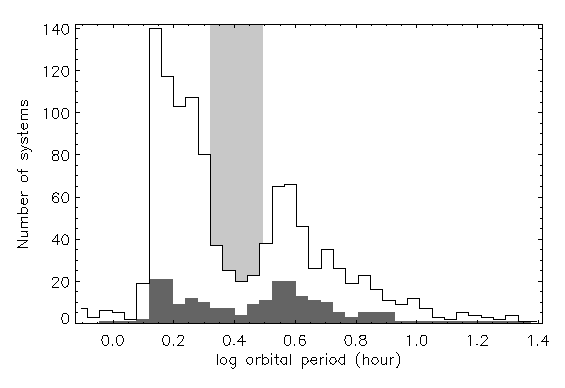
\includegraphics[width=\columnwidth]{figures/introduction/pd-rk.eps}
    \caption{Reproduced from \citet{southworth2015}, Figure~14. The orbital period distribution of RKCat \citep{RKCat} CVs identified by the SDSS (white histogram) and of the subset of these which are eclipsing (grey histogram). The light grey rectangle delineates the period gap at 2.1 - 3.1 hours. The periods have been collected into histogram bins which are of equal size in log space.}
    \label{fig:period hist}
\end{figure}

The orbital period of a CV can be measured by tracking either their spectroscopic radial velocities (e.g. \citealt{gaensicke2009}), or the timings of repeating features in their lightcurves (e.g. \citealt{Littlefair2008}). Once this has been done for a large enough sample, a histogram of the periods can be plotted. This plot, shown in fig.~\ref{fig:period hist}, is important to understanding how a CV will evolve over time.
There are three immediately obvious features of the plot;
\begin{itemize}
    \item a long period cutoff, as the number of systems taper off after $\sim12$hrs
    \item a period gap at $\sim2-3$hrs
    \item a period minimum at $\sim1$ hour, with a pile-up of systems just above it.
\end{itemize}
Each of these features are discussed in turn.

\subsubsection{The period maximum}
\label{sect:introduction:period maximum}
In order for a system be be a CV, mass must be transferring from a less massive star, onto a compact object, constraining the maximum value of $q$ to $\sim1$, and demanding that the secondary extends out to $\sim R_L$. 

There are three constraints on a CV pertinent to the maximum allowable period. The mass ratio, $q = \frac{M_{\rm donor}}{M_{\rm WD}}$, must be low enough for thermally stable mass transfer ($q < 1.23$, \S\ref{sect:introduction:stability criterion}), the donor radius must be approximately equal to the Roche radius, and maximum mass of a white dwarf is well known to be limited to $\le 1.4M_{\odot}$ before triggering thermonuclear runaway \citep{chandrasekhar1942}.

Now, to find the theoretical period maximum, we simply find the period corresponding to the largest possible donor star. \citet{warner1995} found that the average density, $\rho_{av}$, for objects that fill their $R_L$ follows a robust relationship;
\begin{equation}
    \frac{\rho_{av}}{\rho_{\odot}} = 75.9 P_{orb}^{-2}(h)
\end{equation}
\citet{knigge11} derived a connection between CV secondary mass and radius, $M_2$ \& $R_L$. This can be manipulated to produce a mass-period relationship,
\begin{align}
    \rho_{av} = \frac{3 M_2}{4 \pi R_L^3} &\simeq 75.9 P(h)^{-2} \\
    \frac{R_L}{R_\odot} = C &\cdot \Big( \frac{M_2}{D \cdot M_\odot} \Big) ^{\alpha}
\end{align}
where $C$ and $D$ are constants for a particular regime, i.e., short-period, long-period, or period bouncer, and $\alpha$ is the mass-radius index \citep{Knigge2011b}.
Combining the above gives a pleasingly simple relationship.
\begin{equation}
\label{eqn:MP_relation}
    M_2^{(1-3\alpha)} \propto P^{-2}
\end{equation}

For long-period CVs, $\alpha = 0.67\pm0.04$ \citep{knigge11}, and equation \ref{eqn:MP_relation} becomes $M_2^{1.01} \propto P^{2}$, and larger secondary masses require longer periods. The theoretical maximum secondary mass of $1.4 M_{\odot}$ corresponds to a period of $\sim12$hrs, though in reality these higher masses are rarer and the frequency of CVs at these higher periods begins to drop much earlier, at $\sim6$hrs \citep{gaensicke2009}.


\subsubsection{The period gap}
\label{sect:introduction:period gap}

Between periods of around 2-3 hours, there is a dramatic fall in the number of CVs we detect. Volume-limited samples indicate that this is a real effect and not a selection bias \citep{Kolb1998}. However, the origin of this gap in the period is something of an open problem.

Models indicate that long period systems ($P > 3$h) have far higher mass loss rates than short period systems ($P < 2$h) \citep{ritter1985}. This suggests a significant change in braking mechanisms between the two regimes. 

The disruption of magnetic braking was proposed early on to explain the period gap \citep{rappaport1983, spruit1983}, and relatively shortly after \citet{kolb1993} showed more quantitatively that a sub-class of purely gravitational braking CV systems does not reproduce the observed population. 
Historically, the standard evolutionary path of CVs has involved the secondary becoming fully convective which was thought to disrupt the magnetic field and so cease MB \citep{knigge11}, though this mechanism has frequently been questioned. \todo{Gather references}

It is important to develop diagnostics for the nature of the period gap, and \citet{smith1998} show how spectral analysis could yield an accurate observed mass-radius relation for donor stars in CVs as evidence for MB, though they lacked the observations to apply their method. The mass-radius relation would later be carried out by \citet{knigge11}.
\citet{Davis2008} used population synthesis to demonstrate that, if the period gap is caused by disrupted MB, this may affect the mass function of quiescent CVs that are moving through the gap. They expect an excess of non-transferring CVs over low mass post-common envelope CVs that emerge from the common envelope phase directly into the period gap. These should form at a predictable rate across $q$, but due to the slow crossing of quiescent CVs, the latter `pile up' in the gap - a detectable effect observed by \citet{zorotovic2011}.

The system is still subject to gravitational radiation, however, so gradually evolves back towards shorter periods. Once the secondary reconnects with its Roche lobe, mass transfer resumes and the system again presents itself as a CV, emerging from the period gap at a $\sim2$hr period \citep{kolb2002}.

\subsubsection{The period minimum, and period bouncer systems}
\label{sect:introduction:period minimum and bouncers}

The period minimum was first predicted by \citet{rappaport1982}, and can be understood by considering the two governing timescales affecting the secondary. 
For donors with masses above $\sim0.1 M_{\odot}$, the donor is contracting in response to mass loss. 
As this proceeds, both $\tau_{therm}$ and $\tau_{\dot M}$ are increasing (the latter due to $\dot M_2 / M_2$ rising as the period shrinks). However, $\tau_{therm}$ rises faster, and at a period of $\sim80$ minutes \citep{ritter1998, McAllister2019}, $\tau_{therm}$ exceeds $\tau_{\dot M}$, causing the donor to lose mass adiabatically and expand rather than contract in respose to mass loss.
This allows the donor to remain in contact with its Roche Lobe when mass loss raises it to a higher orbit, and the system evolves to longer periods over time.

More quantitatively, as the components of a short period CV move closer together and the donor falls in mass, $\tau_{therm}$ and $\tau_{\dot M}$ become more out of balance, corresponding to $\alpha$ in equation \ref{eqn:MP_relation} decreasing \citep{Knigge2011b}. A main-sequence star will have $\alpha \sim 1$, but a secondary subjected to fast, adiabatic mass loss will have $\alpha \simeq -1/3$. Looking at the gradient of equation \ref{eqn:MP_relation}, the existence of a period minimum can be easily seen.
\begin{equation}
    \frac{\dot P}{P} = \frac{(3\alpha - 1)}{2} \frac{\dot M_2}{M_2}
\end{equation}
When $\alpha \le 1/3$, a negative $\dot M$ will produce a \textit{positive} change in $P$, and the donor begins to retreat from the white dwarf \citep{rezzolla2001}. 

This has been confirmed by \citet{knigge11}, who found that for period bouncer CVs, $\alpha = 0.21^{+0.05}_{-0.10}$, giving the following empirical version of equation \ref{eqn:MP_relation} in the post-period minimum regime.
\begin{align}
    M_2 \propto P^{-5.4}
\end{align}


\subsection{Problems with the classical picture}
\label{sect:introduction:modern AML}
A solid knowledge of exactly how and why CVs lose angular momentum has remained surprisingly elusive for several decades now. Early theories established gravitational waves and magnetic braking as the only two sources of AML \todo{ref}, but attempts to quantify this with evolutionary models \citep{knigge11} and population synthesis models \todo{ref} consistently fall short, as outlined in \S\ref{sect:introduction:AMLMechs}. Gravitational losses are well understood, and have been independantly observed and studied, but the sources and consequences of magnetism in a stellar context is not so easy. 

The spin rate and masses of CV donors is not seen in the singleton stars that are usually used to characterise magnetic braking \citep{rappaport1983,matt2015,garraffo2018a}. 
In addition, the disruption of magnetic braking is often motivated by the donor transitioning to a fully convective state, but X-ray emission level is a diagnostic of magnetic flux \citep{pevtsov2003}, and \citet{wright2016} found that the X-ray flux of CVs is similar between fully convective and non-convective main-sequence stars, implying a similar magnetic field strength. Furthermore, disagreement between observational and theoretical period gap and minimum locations \citep{knigge11} has left the disrupted MB model an area of active research. 
\citet{garraffo2018} recently proposed that the magnetic field does not weaken, but rather becomes more complex which reduces the efficiency of MB. This concept is discussed quantitavely in \S\ref{sect:introduction:Garraffo MB prescription}.


\subsection{The missing AML problem}

The evolution of CVs is driven by the donor stars. The orbital period is determined by the mass-radius relationship of the donor under mass loss, and the decay of the orbit should simply result directly from the two braking mechanisms (gravitational and magnetic). Figure~\todo{put in the one from my 2021 paper here} shows the relationship between the donor mass and orbital period, and the single unified CV track can be seen. Stellar evolution models can be built to try and reproduce this track, and indeed at long periods, our understanding of those mechanisms seem robust enough to produce models that satisfy observations. The period gap can, with some manual tweaks, also be reproduced with some accuracy. Unfortunately, at short periods ($\lesssim 2 hours$), the data begin to diverge from models. 

\S\ref{sect:introduction:Summary of how AML and Mdot drive period evolution} describes how the donor has its mass-radius relation altered by the presence of continued mass loss. The donor is larger than a singleton of the same mass, as the mass loss timescale is comparable to the thermal timescale and the donor is not quite able to maintain thermal equilibrium \citep{knigge11}. The degree of this inflation increases with more mass loss. As mass loss is driven by AML, it follows that a CV donor that has stronger AML will have a larger radius, and therefore sit at a longer period than a CV with weaker AML, altering the gradient of the tracks in Figure~\ref{fig:introduction:Knigge 2011 figure 9} at periods of $\lesssim 3h$. In this way, the shape of the tracks in Figure~\ref{fig:introduction:Knigge 2011 figure 9} is a diagnostic of the form of AML experienced by a CV across its lifetime \citep{knigge11}.
This also moves the period minimum to longer periods. The period minimum is caused by the donor's $\tau_{therm}$ becoming longer than $\tau_{\dot M}$, and since a faster mass loss will result in a shorter mass loss timescale, this crossover point is moved to higher masses and therefore longer periods. This is compounded by the faster mass loss resulting in more severe bloating of the donor star, so a donor of the same mass will connect to its Roche lobe at longer periods. 

\citet{knigge11} used took observations of donor masses and radii, with masses determined by either eclipse modelling, or the $\epsilon - q$ superhumper relationship, and radii are readily found from equating the donor radius to the expected Roche lobe radius. 
With donor properties for masses $\sim 0.1 - 1 M_\odot$, an unknown additional source of AML was added to their models, simply scaled relative to gravitational braking. This source is motivated by the disagreement between data and the model that omits this source. \citet{knigge11} find that the best-fit model to their data uses an excess braking that is $2.47 \times \dot J_{GR}$, where $\dot J_{GR}$ is AML due to gravity. Figure~\ref{fig:introduction:Knigge 2011 figure 9} is reproduced from their work, and shows the significant improvement in agreement with data.

\begin{figure}
    \centering
    \includegraphics[width=\textwidth, trim={0 2cm 0 2cm}]{figures/introduction/Knigge11_fig9.pdf}
    \caption{Reproduced from \citet{knigge11}. {Black} markers are data from superhumpers, {Red} markers are data from eclipsers. {Crosses} denote candidate period bouncer CVs, {Squares} are short-period CVs, and {Circles} are long period CVs. {Open symbols} are omitted from their analysis due to lying in the period gap. The {Dashed Black lines} are their `standard', naiive model, and the {Solid Red line} includes an empirically determined excess AML source, scaled to gravitational wave braking. In the top panel, the {Vertical black line} signifies the observed period minimum, with the grey region as the FWHM of the period spike as measured in \citet{gaensicke2009}.}
    \label{fig:introduction:Knigge 2011 figure 9}
\end{figure}

\citet{Pala2017a} used the effective temperatures of the white dwarfs to probe CV evolution. The white dwarf temperature can be enhanced by accretion, so a hotter white dwarf suggests a higher mass transfer rate. This is sensitive to changes in $\dot M$ on short timescales, but still provides a valuable insight. \citet{Pala2017a} compare their white dwarf temperatures (and therefore mass transfer rates, and therefore AML rates) to MESA CV evolutionary tracks, and find that their observed temperatures are poorly described by only gravitational AML, but are more well-fitted by models that includes excess AML equivalent to gravitational losses, i.e. double-strength gravitational AML. Their analysis is useful but not wholly convincing, as the white dwarf temperatures are both quite poorly constrained, and sensitive to short-term variations in accretion rate that are known to occur\todo{cite}. In addition, the scaling of excess AML in relation to gravitational losses is not a free parameter in their analysis, and is only presented in the context of being obviously better by eye, rather than being tailored to the data.

The disagreement between theory and observation at short periods indicates that our understanding of AML in this regime is lacking, and a few proposals to rectify this have been suggested.

The obvious solution to the problem of missing AML is that we simply do not understand magnetism well enough to say that it ceases below the period gap. The donor may retain a residual magnetic field strong enough to drive some weaker form of magnetic braking that remains after the bulk of magnetic braking ceases. This is called Residual Magnetic Braking (RMB). Some evidence for RMB has been found in binary population synthesis models that focus on magnetic CVs \citep{belloni2020}. This approach asserts that a strong magnetic field from the white dwarf significantly reduces the effectiveness of magnetic braking by trapping a large fraction of the wind within the system, preventing it from carrying angular momentum away. The models that include this result in a better fit to key CV observables, specifically the orbital period distribution, white dwarf temperature distribution, and space density. While this theory does not apply to CVs in general, as the majority of systems do not have white dwarfs with strong enough magnetic fields, it has been suggested that a similar process could  occur on the donor \citep{garraffo2018}. 

The period gap is frequently attributed to the donor becoming fully convective, and this triggering a large reduction in magnetic field strength. However, observations of field M dwarfs of the same mass, with convective envelopes, are seen with key tracers of magnetism. Specifically, X-ray observations find that the coronal magnetic energy dissipation of fully convective stars is similar to non-convective stars \citep{wright2016}, and Zeeman-Doppler imaging of rapidly rotating M dwarfs indicate that the complexity of surface magnetic fields increases alongside rotation rate (e.g. \citealt{donati2003,donati2009,marsden2011,waite2011,waite2015}). Together, these observations strongly indicate that the disrupted magnetic braking model commonly accepted is ill-motivated, and may be more closely tied to field complexity than field strength \citep{garraffo2018}. If the gap is indeed driven by a sudden increase in field complexity, then it is reasonable to assume that magnetic braking remains significant after the system emerges from the period gap. However, this is not the only explanation for excess AML, and another strong candidate is consequential AML.


\subsection{Consequential AML}
\label{sect:introduction:CAML}

At its core, consequential AML (CAML) is a simple concept. It's known that the accreted material on CV white dwarfs detonates, and the majority of this material is lost from the system \citep{McAllister2019}. This will carry with it angular momentum, and so forms a third source of AML \citep{king1995,schenker1998}. By modelling CV evolution including this process, several issues of older CV population synthesis and evolutionary models can be solved at once \citep{Schreiber2016}. These issues are: 
\begin{enumerate}
    \item the observed mass of CV white dwarfs is systematically higher than singleton white dwarfs (e.g. \citealt{McAllister2019,pala2020});
    \item since the short period regime has much lower AML rates, CVs should spend most of their time below the period gap, and $\sim 99\%$ of CVs are expected to be short period \citep{kolb1993a}, but observations see a roughly even distribution between long and short period systems \citep{knigge2006};
    \item under purely gravitational losses, the period minimum was first calculated at $\sim 67$ minutes \citep{kolb99}, but is observed at $\sim 79$ minutes \citep{McAllister2019};
    \item the space density of CVs is roughly 1-2 orders of magnitude lower than population synthesis models predict.
\end{enumerate} 
The introduction of a modified, empirically calibrated CAML can account for these issues, making a compelling case for its validity. 

The maximum dynamically stable mass transfer rate of a CV is a function of $q$, related via the adiabatic mass-radius exponent, $\alpha_{ad}$, and the mass-radius exponent of the Roche radius, $\alpha_{L}$. Where the two intersect forms a threshold beyond which runaway mass transfer (much like the pre-CV common envelope phase) is triggered, and most likely results in a merger between the two bodies.
\begin{equation}
    \label{eqn:introduction:CAML stability threshold}
    \alpha_{ad} = \frac{{\rm d} ln(R_2)}{{\rm d} ln(M_2)}_{ad} = \frac{{\rm d} ln(R_L)}{{\rm d} ln(M_2)} = \alpha_L
\end{equation}
Where $\alpha_{ad}$ for convective stars is $-1/3$. Recalling the Eggleton approximation for the Roche radius, Equation~\ref{eqn:eggleton approximation}, we can find $\alpha_{ad}(q)$ \citep{Schreiber2016} in the absence of CAML,
\begin{equation}
    \alpha_{ad} = \frac{2}{3}\frac{ln(1+q^{1/3}) - \frac{1}{2}\frac{q^{1/3}}{1+q^{1/3}}}{0.6q^{2/3} + ln(1+q^{1/3})} (1 + q) + 2(q - 1) = -1/3
\end{equation}
Solving this equation gives a critical maximum value of $q < 0.634$. However, under the additional CAML, an extra source of $\dot J$ is introduced, $\dot J_{CAML}$.
\begin{equation}
    \frac{\dot J_{CAML}}{J} = \nu \frac{\dot M_2}{M_2}
\end{equation}
Here, $\nu = M_2^2 / (M_1(M_1 + M_2))$ and describes the angular momentum carried by ejected nova material, defined to be teh same as teh white dwarf momentum.
The right hand side of Equation~\ref{eqn:introduction:CAML stability threshold} is then altered by the increased AML rate.
\begin{equation}
    \alpha_{ad} = \frac{2}{3} \Bigg( \frac{ln(1+q^{1/3}) - \frac{1}{2}\frac{q^{1/3}}{1+q^{1/3}}}{0.6q^{2/3} + ln(1+q^{1/3})} \Bigg) + 2\nu + \frac{M_2}{M_1 + M_2} - 2
\end{equation}
The effect of this altered form of $\alpha_{ad}$ is that CVs with higher mass ratios are stable. Models with this prescription perform worse than non-CAML models. Binary population synthesis models by \citet{Schreiber2016} demonstrate that this model is not accurate to observations, producing {\it more} CVs with low mass donors than the non-CAML model. However, by altering the form of $\nu$ so that it is no longer tied to the white dwarf's angular momentum, a much better agreement with observations can be reached. This is the empirical CAML model, or eCAML.

$\nu$ is altered to a simple function of the white dwarf primary mass,
\begin{equation}
    \label{eqn:introduction:eCAML nu}
    \nu (M_1) = \frac{C}{M_1}
\end{equation}
where $C$ is an arbitrary constant chosen to best reflect observations, and \citep{Schreiber2016} adopt values of $C = 0.3 - 0.4$. The inverse relationship of more CAML at lower white dwarf masses is motivated by lower mass systems being able to retain less nova material, so more can be ejected and so carry more angular momentum. 

With eCAML, the dynamically unstable region \todo{put in their fig 1+2} is expanded. This has the important effect of making CVs with low-mass white dwarfs prone to dynamically unstable mass transfer, removing them from the CV population -- this simultaneously answers the question of CV white dwarfs being more massive than expected, and also vastly lowers the space density \citep{belloni2018}. Finally, the majority of systems that are now dynamically unstable are short-period CVs, so the observed period distribution is significantly more well-reproduced\todo{point at the Schreiber fig 2 panel}. 

Some observational evidence for eCAML has recently been uncovered by \citet{Pala2021}, where an inverse correlation between white dwarf mass and mass loss rate was observed. This is in line with Equation~\ref{eqn:introduction:eCAML nu}. 
Also, low mass ($< 0.5 M_\odot$) helium-core white dwarfs are expected to be formed in binaries, but are frequently observed as singletons. The merger scenario under eCAML provides a neat explanation for this \citep{zorotovic2017}
In addition to this, \citet{sparks2021} observed the spectra of CV donors and found significant non-solar abundances. This indicates that after nova outbursts, some of the nova-processed material is retained in the system long enough to be accreted onto the donor, and is supportive of lower mass white dwarfs having a lower eCAML contribution. In addition to supporting traditional eCAML this way, the re-accretion phase of the nova material provides a frictional AML mechanism \citep{Schreiber2016,sparks2021}, as the ejecta briefly forms a common envelope phase, as an alternative CAML mechanism to nova ejecta being completely lost from the binary. 


\subsection{Magnetic Braking}
\label{sect:introduction:magnetic braking}

Consider a blob of this charged wind material, moving with some sideways velocity in the plane of the orbit, almost certainly slower than the magnetic field lines. 
The blob will interact with the field and accelerated to co-rotate with them.
This higher velocity causes it to move outwards, to a higher orbit, where the field lines are moving even faster, accelerating the blob more. 
The wind then robs the star associated with the magnetic field of rotational angular momentum and its spin rate is slowed. The close proximity of the binary means that tidal effects are strong, and the donor is spun up again by robbing the orbit of angular momentum, reducing their separation and hardening the binary further \citep{verbunt1981}.

As an aside, \citet{wickramasinghe1996} presented theoretical motivation that CVs can have too strong a magnetic field to allow magnetic braking. Open field lines are necessary for wind to escape the system, so too strong a white dwarf magnetic field can trap the ionised gas in-system, suppressing the wind of the secondary. This Magnetic CV subclass is briefly described in \S\ref{sect:introduction:magnetic CVs}.

As the magnetic braking mechanism is a direct consequence of the donor star spinning down, the CV community is able to borrow insights from adjacent fields of study. The majority of M dwarfs experience some form of spin-down under magnetic braking \todo{cite this}, so observations of the magnetic field strengths of singletons should inform the efficacy of magnetic braking in CV binaries\todo{cite this}. Unfortunately, the typical CV rotational period is on the order of a few hours, and singleton M dwarfs are considered extremely fast rotators with periods of a day\todo{cite this}. Observations of singletons simply do not reach to the extremely low mass, rapid rotations that are frequently seen in CVs, so we are forced to rely on extrapolation and theory.

This carries with it some major practical issues. One is that while the broad effects of magnetic fields is relatively easy to intuit, quantitative physical understanding the mechanics and origins of magnetic fields is difficult, involving fluid dynamics, considering interactions with the accretion disc, and magnetism acting on large systems, which quickly become prohibitive to model and is usually handled with one of a variety of recipes. \citealt{knigge11} contains a detailed compilation of some older approaches, but the decade since has seen a few newer methodologies emerge. Here, two recent magnetic braking prescriptions are described in moderate detail: the \citet{matt2015} prescription, and the \citet{garraffo2018a} prescription. For a more complete, detailed summary of the modern understanding of M dwarf magnetic fields refer to \citet{kochukhov2021}. 


\subsubsection{Matt prescription for magnetic torque}
\label{sect:introduction:matt braking}

In \citet{matt2015}, an empirical prescription is derived that relates the torque felt by a low mass main sequence star to that stars' mass, radius, and Rossby number. The Rossby number is a fluid dynamics term for the ratio between the inertial and Coriolis force terms of the Navier-Stokes equations. A small Rossby number indicates a system dominated by Coriolis effects, and a large Rossby number indicates that centrifugal and inertial forces dominate. The Rossby number of a main sequence star can be calculated from $\Omega$, it's angular rotation rate, and $\tau_{\rm cz}$, the convective turnover timescale.
\begin{equation}
    \label{eqn:introduction:rossby number}
    {\rm Ro} = (\Omega \cdot \tau_{\rm cz})^{-1}
\end{equation}
Through the Rossby number, the effectiveness of magnetic braking is tied to rotation, which is extremely fast in CVs, and stellar mass and age, which affect $\tau_{\rm cz}$.

Their work makes use of observations of stars with masses less than $0.15 - 1.3 M_\odot$ and span ages of $\sim 10^{6-9}$ yrs, that have had their rotation periods measured. This dataset is used to calibrate a theoretically motivated empirical prescription for magnetic braking. There is some evidence for a saturation of magnetic activity below a critical Rossby value (a.k.a. above a critical rotational period) \citep{reiners2009}, where magnetic activity seems to no longer respond to changes in rotation. \citet{matt2015} adopt two generic relationships, 
\begin{equation}
    \bigg(\frac{B_*}{B_\odot}\bigg)^{4m} \bigg(\frac{\dot M_\omega}{\dot M_\odot}\bigg)^{1-2m} = Q \bigg(\frac{\rm Ro_\odot}{\rm Ro} \bigg)^{p}
\end{equation}
in the unsaturated regime, and 
\begin{equation}
    \bigg(\frac{B_*}{B_\odot}\bigg)^{4m} \bigg(\frac{\dot M_\omega}{\dot M_\odot}\bigg)^{1-2m} = Q \chi^{p}
\end{equation}
in the saturated regime. Here, $M_\omega$ is the global mass outflow rate, $B_*$ is the magnetic field strength at the stellar surface, and $M_\omega$ is the total mass outflow rate. The $m$ exponent is determined by the field geometry and wind acceleration profile, but functionally is a tuning parameter that likely falls in the range of $0.20 < m < 0.25$ \citep{matt2015}. The $p$ exponent encodes the dependence of magnetism on the Rossby number, $\rm Ro$, and is assigned as $p = 2$. $\chi$ is the inverse critical Rossby number for saturation, for which \citet{matt2015} adopt a value of $10$. $Q$ is a generic scale factor that the authors fit to observations.

The authors use these equations to eventually derive the spin rates for main sequence stars at some time $t$ after their initial spin period, $\Omega_i$, 
\begin{equation}
    \lim_{\Omega_* \gg \Omega_{\rm sat}} \bigg(\frac{\Omega_*}{\Omega_\odot}\bigg) \rightarrow \bigg(\frac{\tau_{\rm unsat}}{t}\bigg)^{\frac{1}{p}}
\end{equation}
\begin{equation}
    \Omega_* = \Omega_i \cdot e^{-t/\tau_{\rm sat}}
\end{equation}
for a rotation period of $\Omega_*$, and the threshold for saturation at $\Omega_{\rm sat}$. The two $\tau$ factors, $\tau_{\rm sat}$ and $\tau_{\rm unsat}$, are the spin-down timescales in the saturated and unsaturated regimes, and $\tau_{\rm sat} \ll \tau_{\rm unsat}$.

The authors take observations of two clusters, the $\sim 5$ Myr old ONC cluster and the $\sim 580$ Myr old Praesepe cluster, and use the first as initial conditions and the second as target distribution to reproduce. Figure~\ref{fig:introduction:Matt 2015 figure 2} is taken from \citet{matt2015}, and compares the initial and final conditions of their synthetic cluster model compared to these two boundary conditions. During the first few tens of Myrs of this model, the stars in the synthetic cluster are spun up as they contract, lowering their periods by factors of $\sim 5-10$. After this initial phase, which is much shorter than the spin down timescales, the more long-term spin evolution begins.

\begin{figure}[!tbp]
    \centering
    \begin{minipage}[b]{\textwidth}
        \centering
        \includegraphics[width=0.8\textwidth]{figures/introduction/matt_2015_fig2a.pdf}
    \end{minipage}
    \begin{minipage}[b]{\textwidth}
        \centering
        \includegraphics[width=0.8\textwidth]{figures/introduction/matt_2015_fig2b.pdf}
    \end{minipage}
    \caption{Figure taken from \citet{matt2015}. Red crosses are observations of the ONC ({\it top}) and Praesepe ({\it bottom}) cluster stars. Black diamonds are synthetic cluster stars. In the bottom panel, the solid green line is the theoretical asymptotic spin rate of unsaturated stars and the dotted blue line delimits magnetically saturated and unsaturated stars.}
    \label{fig:introduction:Matt 2015 figure 2}
\end{figure}

The agreement between the synthetic cluster and the Praesepe cluster at 574 Mrys is impressive. Above $\sim 0.8 M_\odot$, stars converge on a single narrow mass - period track just as is seen in the observations, and the large scatter below $\sim 0.8 M_\odot$ is also reproduced. Also, just as is seen in the cluster observations of Praesepe, the fastest rotators are those with the lowest masses. Both of these features arise from the transition from saturated braking, to unsaturated braking \citep{matt2015}. 

At formation, almost all stars are experiencing saturated magnetic braking. The single narrow track arises from higher mass stars spinning down faster than lower mass stars, bringing them down to the much less efficient unsaturated braking regime sooner. The pile-up of systems then produces the narrow track. The mass dependancy of this track comes from the fact that $\tau_{unsat}$ is shorter for lower mass stars.
The broad population of low mass rapid rotators is a direct result of the broad initial conditions, which span an order of magnitude themselves, and the longer spin-down time of lower mass stars in the saturated regime allowing them to remain at high rotation rates for longer. 

However, this model does fail in a few key respects. In the right panel of Figure~\ref{fig:introduction:Matt 2015 figure 2}, a small population of very slow rotators can be seen at $\sim 0.4 M_\odot$. The slower rotation rates of these stars suggests an alternative spin-down mechanism. The inverse problem is seen at $\sim 0.7 M_\odot$, where a handful of stars are seen rotating {\it faster} than predicted by any of the synthetic cluster stars, suggesting that magnetic braking is not as effective in their case.
More importantly for the CV field, the parameter space of CVs is completely uncovered, as CVs have rotation periods of $< 0.2$ days on the high end, and the systems that this work concerns have periods of $\lesssim 0.07$ days. While this would firmly place CVs in the saturated regime, there is evidence of a `supersaturated' regime at extreme rotation periods that may be relevant to CV donors \citep{James2000, Wright2011, Argiroffi2016}. This possibility is also noted by \citet{Gossage2021} when outlining best practice use of this prescription in the stellar evolution code MESA, though the subject is not a settled matter and competing evidence for the {\it lack} of supersaturation has been reported by \citet{jeffries2011}.


\subsubsection{Garraffo prescription for magnetic torque}
\label{sect:introduction:Garraffo MB prescription}

The \citet{garraffo2018a} model considers the morphology of the magnetic field to also be important the the strength of magnetic braking, based on the work by \citet{garraffo2015}. The primary justification for this inclusion is observations of open clusters of a known age, where a bimodality is seen in the rotation rates of stars of similar masses\todo{Cite skumanich gap}. Some stars appear to be fast rotators, and some are slow rotators, and there is a dearth of systems between the two. 
Previous attempts to model this bimodality have relied on a random, unexplained transition between an efficient braking state, and an inefficient braking state \citep{spada2011,reiners2012, gallet2013}, and \citet{garraffo2018a} expand on this by offering a shift in magnetic field morphology as the underlying trigger.

Their formalisation of this is based on two assumptions. They assume that stars with the dipolar component of the magnetic field dominating  follow a known spin-down law, with a mass dependence reflecting $\tau_{\rm cz}$\todo{cite Skumanich}. Second, they assume that there is some relationship between field morphology and stellar spin rate. Specifically, that stars rotating more rapidly have more complex magnetic fields. This is formalised via an AML rate, $\dot J$,
\begin{equation}
    \dot J = \dot J_{\rm dipole}Q_J(n)
\end{equation}
where $\dot J_{\rm dipole}$ is the dipole loss under the Skumanich law, $\dot J_{\rm dipole} \propto \Omega^3 \tau$. $Q_J$ is a modulating factor that encapsulates the field complexity at the stellar surface, and is controlled by the complexity factor, $n$, which has its own prescription. \citet{garraffo2016} derive an equation for $Q_J$, based on fitting the results of simulations with varying field complexities.\todo{Explain the model, and the origin of these numbers before reporting the relationship}
\begin{equation}
    \label{eqn:introduction:garraffo complexity modulation}
    Q_J(n) = 4.05 e^{-1.4n} + \frac{n-1}{60Bn}
\end{equation}
Where $B$ is the magnetic field strength at the stellar surface. As the second term is only significant for $n > 7$, \citet{garraffo2018a} consider $n = 7$ as the maximum complexity, consider only the first term of this relation. This is the equivalent of the saturation of magnetic braking from \S\ref{sect:introduction:matt braking}, but here is contingent on field complexity rather than $\rm Ro$. 

\citet{garraffo2018a} suggest the following relation between $\rm Ro$ and $n$,
\begin{equation}
    \label{eqn:introduction:garraffo field complexity}
    n = 1 + \frac{0.02}{\rm Ro} + 2 {\rm Ro}
\end{equation}
based on observations of open clusters. The three terms reflect three aspects of the magnetic braking model - the minimum complexity is defined as $n \equiv 1$, the first factor encodes stars with small $\rm Ro$ having large $n$ (e.g. young, fast rotators), and the third term gives stars with large $\rm Ro$ similarly large $n$. 
This prescription means that the AML of a star is purely a function of its Rossby number, c.f. Equation~\ref{eqn:introduction:rossby number}.

Similarly to \citet{matt2015}, \citet{garraffo2018a} run a population synthesis model to compare to observations using initial conditions taken from the 13 Myr old h Persei cluster \citep{moraux2013}, but the authors show that differences between alternative initial conditions do not survive longer than 200 Myrs. Observations of stellar rotation periods and colour from several clusters with known ages are then compared to the synthetic population.

The resulting distribution does recover the Skumanich bifurcation observed in open clusters, reproducing the fast and slow rotating populations and the gap between them, though the large uncertainty in the age of the cluster does introduce some discrepancy. 
In addition, the synthetic cluster does not consider the effects of close binary stars, which will affect the spin-down rate through tidal effects. As the comparison to data is done with color, filtering out binaries is difficult. However, this effect is ignored by the author, as there is evidence that the binary fraction in open clusters is low \citep{meibom2007}.
The mass dependency of this track is also reproduced by the model, and Figure~\ref{fig:introduction:garraffo 2018a fig 4}.

\begin{figure}
    \centering
    \includegraphics[width=0.8\textwidth, trim={0 5cm 0 5cm}]{figures/introduction/garraffo2018_M37_346_hPer.pdf}
    \caption{Example comparison between synthetic and observed cluster populations taken from \citet{garraffo2018a}. Red points are observations of M37, which has its age measured at $\sim 346 - 550$ Myrs. Blue points are the probability distribution of the synthetic cluster population from \citet{garraffo2018a}.}
    \label{fig:introduction:garraffo 2018a fig 4}
\end{figure}

The \citet{garraffo2018a} prescription is simpler in concept than the \citet{matt2015} prescription, and both prescriptions perform well. However, neither formulation covers the parameter space of CV donors, and both are semi-empirical with some arbitrary decisions made in order to fit data. This makes both approaches highly vulnerable to extrapolation errors and difficult to trust in the context of CV evolution, especially in the short period regime.


\subsubsection{Comparisons to the Rappaport, Verbundt and Joss model}

We can examine the differences between these prescriptions in the case of CV evolution by applying them to a donor evolutionary track, and \citet{knigge11} has constructed a donor sequence using their own models that reasonably accurately reproduces observations. The masses, radii, and periods along the sequence are given, so the would-be effects of the magnetic braking prescriptions described above can be calculated. In addition to the two previously discussed prescriptions, the default MESA \citep{Paxton_2015} magnetic braking prescription \citep{rappaport1983} is included. This prescription includes a magnetic braking index, $\gamma$,
\begin{equation}
    \dot J = -3.8\times10^{-30} M R_\odot^4 \bigg( \frac{R}{R_\odot} \bigg) \omega^3
\end{equation}

Note that in the specific case of CVs, period and radius are synonymous with one another, due to the requirement that the donor is in contact with the Roche lobe, and is tidally locked. 

\begin{figure}
    \centering
    \includegraphics[width=\textwidth, trim={1cm 0 0 0}]{figures/introduction/rappaport_matt_magbraking.png}
    \caption{Showing the AML rates, $\dot J$, of three magnetic braking prescriptions, applied to the masses, radii, and spin periods of the `standard' CV donor track of \citet{knigge11}. The vertical black line shows the mass at which \citet{knigge11} enforces the period gap to occur. {\bf Green lines} show the \citet{rappaport1983} magnetic braking prescription, which is the default used in MESA \citep{Paxton_2015}. The {\bf red line} shows the \citet{matt2015} prescription.}
    \label{fig:introduction:rappaport garraffo matt magnetic braking}
\end{figure}

Figure~\ref{fig:introduction:rappaport garraffo matt magnetic braking} shows how the \citet{matt2015} magnetic braking prescription compares to the default MESA mabgnetic braking prescription, from \citet{rappaport1983}. 

The differences between the three prescriptions is clear in both the overall strength of the prescriptions, but also in how they evolve with mass. All the prescriptions shown decrease at lower masses, but at different rates. In the context of CV evolution, a different dropoff rates of magnetic braking would alter the shape of the donor mass-radius sequence, so observations of CV donors should be able to allow us to evaluate the effectiveness of different braking prescriptions.



\section{This work}
\label{sect:introduction:this work}

\chapter{Observations and observational techniques}
% Chapter Template

\label{chpt:observations and observational techniques} % for referencing this chapter elsewhere, use \ref{chpt:label}
\lhead{\emph{Observations, and observational techniques}} % This is for the header on each page - perhaps a shortened title

% In CVs with a sufficiently high inclination ($\gtrsim 80 \deg$, depending on mass ratio) the donor star will eclipse the white dwarf, accretion disc, and bright spot in quick succession once per orbit. Observing and modelling these eclipses, with knowledge of the orbital period and the temperature of the white dwarf, can yield a thorough characterisation of the CV. The methodology for this characterisation is described in detail in \S\ref{chpt:modelling and techniques}, but essentially relies on extracting the white dwarf temperature, mass, and radius from modelled white dwarf colours and the Gaia-reported system parallax, then combining the white dwarf mass and radius with the timing of various eclipse features to find the key parameters of donor mass, donor radius, and orbital separation.\todo{Stu marked this as duplication, but I dont think it is... And I think its necessary setup for the chapter.}
% Since the important observables are colours and the timing of events, to properly characterise a CV we need flux-calibrated, high time resolution, multi-colour photometry of a target.

The work of this thesis has made use of three instruments: ULTRASPEC, ULTRACAM, and HiPERCAM.
These are time-series photometric imaging cameras, capable of taking high-cadence images of the night sky in one, three, or five colours, respectively.
The observed eclipses typically span around 30 minutes and observations need to measure flux changes on timescales of a few seconds to resolve the eclipse.
Crucially, HiPERCAM and ULTRACAM make their multi-colour images simultaneously, which removes the possibility of changes in brightness in the disc or bright spot polluting the white dwarf colour measurement, making them ideal instruments for this analysis.


\section{Instruments}
\label{sect:observations:cameras}

The cameras used were mounted on several telescopes across the decade of our observations. These were the Gran Telescopio de Canarias (GTC) on La Palma (with HiPERCAM), the Thai National Telescope (TNT) with ULTRASPEC, the New Technology Telescope (NTT) in Chil\'e (with ULTRACAM). Prior to 2016, ULTRACAM was hosted on the William Herschel Telescope (WHT), on La Palma. Section \ref{sect:observing:observation catalogue} details what instrument/telescope combination was used for each observation used in this thesis.


\subsection{HiPERCAM}
\label{sect:observations:hipercam}

HiPERCAM is a quintuple-beam optical imaging camera that saw first light on the WHT in 2017, and is sensitive to wavelengths from $320 - 1060 \rm nm$ \citep{dhillon2021}.
HiPERCAM uses a system of `Super SDSS' filters ($u_{\rm sup}, g_{\rm sup}, r_{\rm sup}, i_{\rm sup}, z_{\rm sup}$), designed to match the classic SDSS band cutoff wavelengths \citep{fukugita1996}, but allow a higher throughput and so give a more sensitive instrument.
This instrument has a series of dichroic beam-splitters, that sequentially pick off the $u_{\rm sup}, g_{\rm sup}, r_{\rm sup}, i_{\rm sup}, z_{\rm sup}$ bands and funnel each into dedicated cameras that use highly sensitive, low readout noise, Charge-Coupled Devices (CCDs) as detectors.
However, this improvement in sensitivity is not constant across the bands, shown in Figure~\ref{fig:observations:superSDSS throughput comparison}, resulting in a small difference between colours observed with HiPERCAM and the SDSS.
Unfortunately, as magnitudes for standard stars are often reported in the classic SDSS photometric system, some work was necessary to color-correct the HiPERCAM observations, which is described in detail in \S\ref{sect:observations:colour correction method}.
\begin{figure}
    \centering
    \includegraphics[width=0.7\textwidth]{figures/observations/plot_dichs_supersdss_asbuilt_v3.png}
    \caption{Taken from \citet{dhillon2021}. Transmission profiles of the as-built HiPERCAM dichroic beam-splitters ({\bf dashed black lines}), the HiPERCAM standard SDSS filters ({\bf dotted lines}), and the HiPERCAM Super SDSS filters ({\bf solid lines}).}
    \label{fig:observations:superSDSS throughput comparison}
\end{figure}

On the GTC, HiPERCAM is capable of detecting sources down to $g_{\rm sup}~\sim~23$ in exposures of only a second, and can achieve $g_{\rm sup}~\sim~28$ with an hour of exposure. This allows observations of fainter CVs than previous studies (e.g. \citealt{McallisterThesis}), and helps target CVs at short periods with faint, low mass donors.
Unfortunately, while HiPERCAM was used to observe eclipses for some systems, no HiPERCAM observations were modelled for this thesis, with observed systems either being in outburst, or not having observable bright spot features, which are essential for modelling.

HiPERCAM is capable of incredibly fast frame rates of up to $\sim 1000 \rm Hz$, though this capability was not used for this work.
However, as part of the effort to achieve this frame rate by reducing dead-time between frames HiPERCAM is capable of exposing a frame while {\it simultaneously} reading out the previous image.
This is achieved by masking half of a CCD, and only exposing with one side. When a frame is finished exposing, it is shuttled across to the masked side (a rapid process, $6.8 - 7.8$ ms) and can be read out during the next exposure time. To compensate up for masking half of a CCD, four CCDs side-by-side are used to make up the full exposing area. As a consequence, HiPERCAM has four sets of readout electronics that operate in tandem.
This virtual elimination of dead-time is a significant benefit when resolving the large, rapid changes in flux during the ingresses and egresses of CV eclipses.



\subsection{ULTRACAM}
\label{sect:observations:ultracam}
o
ULTRACAM is a three-beam optical imager sensitive to wavelengths between $\sim 300 - 1100 \rm nm$, and is the direct predecessor to HiPERCAM \citep{dhillon2007}.
It is similarly built for high-speed photometric studies, but is not capable of the extreme framerates of HiPERCAM, limited to framerates of $\lesssim 500 \rm Hz$.
ULTRACAM uses the same frame transfer readout technique to HiPERCAM, though uses only two CCDs.

ULTRACAM was originally commissioned with SDSS-like $u',g',r',i',z'$ filters, that match the SDSS closely and did not necessitate colour-term corrections. However, in Fubruary 2019 ULTRACAM was upgraded to use the same Super SDSS photometric system used by HiPERCAM. When necessary, observations were translated to the classic SDSS system as described in \S\ref{sect:observations:colour correction method}.
Observing an object with ULTRACAM in more than three bands requires multiple observing runs, and manually swapping filters.


\subsection{ULTRASPEC}
\label{sect:observations:ultraspec}

ULTRASPEC was occasionally used to supplement ULTRACAM and HiPERCAM observations. ULTRASPEC was originally commissioned as a spectrographic cousin of ULTRACAM, using again a frame transfer design, with an electron-multiplying CCD \citep{dhillon2014}.
After a brief proof-of-concept trial as a photometric imager in June 2009, ULTRASPEC was modified to a full-time imaging instrument and mounted on the 2.4m TNT in November 2013, and is now operated by the National Astronomical Research Institute of Thailand (NARIT).

This is a single-colour instrument that uses the $u',g',r',i',z'$ filters, in addition to a wide-band KG5 filter that is approximately equivalent to $u' + g' + r'$. It is also the slowest of the three cameras, but is still capable of high framerates up to $\sim 200 \rm Hz$. However, as ULTRASPEC on the NTT is a somewhat less in-demand instrument than either HiPERCAM or ULTRACAM, it proved useful in two significant respects - to gauge the viability of CV systems before dedicating more valuable HiPERCAM and ULTRACAM observing time (e.g. testing the visibility of eclipse features, checking if a CV is undergoing an outburst), and in acquiring or refining measurements of orbital period.


\section{Data reduction}
\label{sect:observations:data reduction}

All three cameras use CCD detectors, which are a staple of ground-based astronomy due to their high sensitivity, and low noise.
CCDs are made up of a large grid of photosensitive pixels, which release electrons proportionally to the number of photons that fall on them. This signal is then moved pixel-by-pixel into the readout electronics, which is essentially a capacitor that has its voltage measured to determine the number of electrons that were released. This voltage is converted to electron counts with an Analog-to-Digital Converter (ADC), that outputs the corresponding integer number of electrons to the input charge, in Analog-to-Digital Units (ADU).
To extract time-series photometric information from the raw image files, the HiPERCAM data reduction pipeline was used\footnote{Available https://cygnus.astro.warwick.ac.uk/phsaap/hipercam/docs/html/}.

The analysis of this data uses flux-calibrated relative photometry, in which a reference star in the same image as the target is extracted and used as a known-constant flux source. Then, by using the ADU flux ratio between these two sources as the observable, effects from changes in weather, altitude, and seeing conditions are compensated for, since these variations are assumed to affect both the target and reference star equally. By multiplying the ADU ratio between the target and reference stars by the flux in mJy of the reference star, we can calibrate our photometry and produce a lightcurve of the target star.
% Bias and flat field corrections are done for each observation, with calibration frames taken nightly as standard procedure.


\subsubsection{Bias frames}
\label{sect:observations:bias frames}

\begin{figure}
    \centering
    \includegraphics[width=0.7\textwidth]{figures/observations/bias_frame_histogram.pdf}
    \caption{Illustrating the effect of omitting negative values on the average of a distribution. The {\bf black line} is a Gaussian distribution with an average of 5 and a standard deviation of 7. The {\bf vertical dashed line} shows the `true' average of 5 ADU, and the {\bf vertical solid line} shows the average given by an ADC that reports negative electron counts as 0.}
    \label{fig:observations:bias frame histogram}
\end{figure}
The readout electronics of a CCD are not perfect, and contribute a small amount of gaussian noise to each pixel, called readout noise. The ADC is only capable of recording {\it positive integer values}, and rounds negative pixel counts to 0. To illustrate why this is an issue, take the exaggerated example of a readout noise of $7 e^-/{\rm px}$ on a region of the CCD that is stimulated by $5 e^-/{\rm px}$. If negative values are limited to 0, the effect is to increase the average, and Figure~\ref{fig:observations:bias frame histogram} illustrates the effect of discarding negative counts.
This will have a small corrupting effect on low-signal areas of the CCD, significantly corrupting the sky background signal that must be subtracted from the source signal (\S\ref{sect:observations:aperture photometry}). Without proper bias correction, a similar corruption also occurs for the flat field images described below.

To prevent corruption, a small bias voltage is applied to each pixel, raising the null detection value away from zero and preventing noise from giving negative readings.
To then remove this bias voltage from observations, zero second exposures of a masked detector are taken to characterise the bias voltage for each pixel, and are subtracted off each subsequent exposure. These are known as bias frames, and because the structure of the bias is subtly altered by different instrument setups, a new bias frame is taken when instrument options such as binning pixels together when reading them out, or only reading out partial images, are altered.


\subsubsection{Flat fielding}
\label{sect:observations:flat field frames}

The response of each pixel to photons is similar, but not exactly equal. In addition, the optics of the telescope are not perfect and throughput varies across the field of view, a.k.a vignetting.
Dust and imperfections in the telescope optics can also introduce variation across the image, and must also be accounted for.

These effects mean that each exposure the instrument takes is convolved with a constant flat-field response pattern.

In order to characterise and remove the flat-field pattern, an exposure is taken of an image that is known to be uniform in brightness, which will have the flat-field pattern imprinted on it.
The twilight sky forms a highly uniform field in optical bands, so was used as this flat source.

Residual stellar light should still be removed, so to completely eliminate stars from the flat field observation, many exposures are taken while the telescope is being nudged by a small amount every few seconds. Since the stars move pixels between each exposure, calculating the median frame will remove stars from the image, leaving behind only the uniform sky observation imprinted with the flat-field response pattern.
The flat field images are bias corrected to give the final flat image.
Then, by dividing each subsequent exposure by the flat image, we can correct for non-uniformity in the detector response in future images.


\subsubsection{Aperture photometry}
\label{sect:observations:aperture photometry}

While stars are theoretically point sources, we observe them through the atmosphere and the optics of the telescope, which act to spread the light from a star, usually by a few arcseconds even under the best conditions. This spreads light from a star over several pixels. As such, to find the total flux of a star we must sum the contributions from all pixels containing the stars' flux, and ideally subtracting all flux contributed by non-stellar sources.
The HiPERCAM pipeline has two methods for this: `normal' extraction and `optimal' extraction.

The sky background is not perfectly black and in both extraction methods must be removed from the extracted flux of a source. This is done by taking an annulus about each source, and assuming it is solely make up of sky background light (in the case of a nearby object, portions of the annulus can be masked in software and not counted in the sky background).
The inner edge of the annulus is selected to be far enough from the source that none of the target's light is present, and the outer edge is limited by the need to avoid contamination from other sources, and large annuli starting to become sensitive to sky variations across the image.
The average sky signal per pixel is then calculated, and subtracted to isolate the source flux.

Under normal extraction, the user specifies one or more `reference' stars, and one or more `target' stars. The pixel ADU counts around the reference stars as a function of their radial distance to the peak flux are characterised with a Gaussian or Moffat profile. The Full-Width at Half Maximum (FWHM) of this distribution fit is calculated, and all pixels within $x \times \mathrm{FWHM}$ of the peak flux are summed to give the extracted flux of a source, cutting off some fraction of the wings of the flux distribution. Here $x$ is a user-defined parameter, and while in theory a large value of $x$ would be desirable to capture all flux from a source, adding extra pixels increases the readout noise of the detection, and suffers from diminishing returns due to the small amounts of flux contained in the wings.
Also, as the same fraction of light from each source should be lost from both the target sources and reference sources, cutting out these wings should not alter the flux ratio between sources, and the flux ratio is the relevant quantity under relative photometry (see \S\ref{sect:observations:photometric extraction and calibration}).

In many cases, it is preferable to use the `optimal' extraction method, described by \citet{naylor1998}. Here, a weight is taken into account when summing the flux contributions of each pixel based on the {\it expected} contribution to the overall flux.
This can give an improvement of $\sim 10\%$ to the signal-to-noise ratio, especially in faint sources as less weight is given to pixels at the wings of the flux profile, where readout noise and error from the sky background are more significant.
However, in brighter stars with an already high signal-to-noise ratio the improvement is offset by the potential systematic error introduced by any divergence from the model profile fit used. As such, the optimal extraction method is generally used for faint stars, and normal extraction is used for bright stars.



\section{Photometric calibration}
\label{sect:observations:photometric extraction and calibration}

A comparison star in the same frame as the target is used to account for seeing and transparency variations over an observation, and standard stars from \citet{smith2002} were used to transform the lightcurves from ADU to the SDSS $u'g'r'i'z'$ photometric system. At the core of the photometric calibrations is the following expression of the apparent magnitude in some band, $m_{app}$, of a target,
\begin{equation}
    \label{eqn:observations:instrumental magnitude from scratch}
    m_{app} = m_{inst} + \chi k_{ext} + m_{zp} + C_{inst}c_{m}
\end{equation}
where $m_{inst}$ is the instrumental magnitude, $-2.5 \rm log(ADU / {\rm time})$, $\chi$ is the airmass of the observation and $k_{ext}$ is the atmospheric extinction coefficient in the relevant band. $m_{zp}$ is the zero point offset of the instrument, calculated from photometric standard stars, ideally taken on the night of an observation. $c_{m}$ is the colour term correction between the response curve of the instrument, and the target photometric system, and $C_{inst}$ is a diagnostic instrumental colour. Each of these terms must be properly handled, and are discussed in turn.


\subsection{Calculating atmospheric extinction coefficients}
\label{sectobservations:calculating atmospheric extinction}

Atmospheric extinction was calculated using the longest continuous observation available within a reasonable time from target observations.

To calculate the atmospheric extinction coefficients, aperture photometery was extracted for five sources in these long observations, and the instrumental magnitude, $m_{\rm inst}$, vs airmass, $\chi$, was fit with a straight line for each source.
The gradients of these lines are the atmospheric extinction coefficients, $k_{\rm ext}$, for the relevant band, and the y-intercept is the instrumental magnitude of that object above the atmosphere, $m_{\rm inst,0}$:
\begin{align}
    \label{eqn:observations:basic magnitude equation}
    m_{\rm inst} =& m_{\rm inst,0} + \chi k_{\rm ext}
\end{align}

% \begin{table}
%     \centering
%     \caption{Typical atmospheric extinction coefficients for La Silla, derived from ULTRACAM/NTT observations.}
%     \label{table:atmos_extinction}
%     \begin{tabular}{cccc}
%         \hline
%         Date of Observation & Airmass Range & Band & $k_{ext}$ \\
%         \hline
%         \hline
%         14 Oct 2018   & 1.30-1.98 & $u_{\rm reg}$ & $0.4476$ \\
%                       &           & $g_{\rm reg}$ & $0.1776$ \\
%                       &           & $r_{\rm reg}$ & $0.0861$ \\
%         \hline
%         30 Sept 2019  & 1.03-1.63 & $u_{\rm sup}$ & $0.4867$ \\
%                       &           & $g_{\rm sup}$ & $0.1803$ \\
%                       &           & $r_{\rm sup}$ & $0.0713$ \\
%         \hline
%     \end{tabular}
% \end{table}


\subsection{Transformations between filter systems}
\label{sect:observations:colour correction method}

ULTRACAM and HiPERCAM use an SDSS-\emph{like} filter system with higher efficiency bandpasses, referred to as Super SDSS. There are three relevant photometric systems:
\begin{itemize}
\item SDSS filters, $u', g', r', i', z'$;
\item ULTRACAM/ULTRASPEC SDSS-like, $u_{\rm reg}, g_{\rm reg}, r_{\rm reg}, i_{\rm reg}, z_{\rm reg}$;
\item HiPERCAM/ULTRACAM Super SDSS, $u_{\rm sup}, g_{\rm sup}, r_{\rm sup}, i_{\rm sup}, z_{\rm sup}$.
\end{itemize}

Note that we have no $z$ band observations, so the $z$ band is omitted hereafter.
We aim to place our photometery in the SDSS $u'g'r'i'$ system, as this is the system later used by the white dwarf atmospheric models, and allows data from different instruments to be either binned together, or modelled simultaneously c.f. \S\ref{sect:modelling:optimising eclipse model parameters}. The $u_{\rm reg}, g_{\rm reg}, r_{\rm reg}, i_{\rm reg}$\ filters were sufficiently similar to standard SDSS filters that the uncorrected magnitudes of standard reference stars from \citet{smith2002} could be used to calibrate absolute photometery without issue. However, with the new filters, there was concern that the different shape of the sensitivity curves, particularly in the $u'$\ band, differ enough from the SDSS filters to cause issues with our photometric calibration. Figure~\ref{fig:sdss vs super filters} illustrates the change in throughput between the SDSS photometric system, and the Super SDSS filters, on ULTRACAM on the NTT.
\begin{figure}
    \centering
    \includegraphics[width=\columnwidth]{figures/observations/bandpass_diffs_SDSS_dots_UCAMNTT_solid.pdf}
    \caption{The differences in photometric throughput in terms of registered ADU, for SDSS filter system ({\bf dotted lines}), and ULTRACAM Super SDSS filters, for ULTRACAM mounted on the NTT ({\bf solid lines}). Blue: $u$ bands, Green: $g$ bands, Red: $r$ bands, Black: $i$ bands. Both throughputs include atmospheric extinction of $\chi = 1.3$.}
    \label{fig:sdss vs super filters}
\end{figure}

To perform the colour corrections, Equation~\ref{eqn:observations:basic magnitude equation} for the magnitude of a star was used with the addition of a colour term. Using the $g'$\ band as an example:
\begin{equation}
    \label{eqn:observations:magnitude with colour term}
    g' = g_{\rm inst} + \chi k_{\rm ext} + g_{\rm zp} + c_{\rm g, sup}(g'-r')
\end{equation}
where $g_{\rm zp}$\ is the zero point, $g_{\rm inst} = -2.5 \rm log(ADU_{\rm exp}/{\it t}_{\rm exp})$
for an exposure time of $t_{\rm exp}$, and $c_{\rm g, sup}$\ is the colour term correction gradient. In theory, the atmospheric extinction term also has some colour dependency, as extinction varies with wavelength. However, the effect is negligible between these photometric systems, so it is omitted.

The optical path of each system was simulated using the \texttt{pysynphot} package, with measured throughputs of all ULTRACAM and HiPERCAM components in the optical path. Precomputed stellar models from \citet{Dotter2016} and \citet{Choi2016} were used to generate the $T_{\rm eff}$ and $\log(g)$ values of an $8.5$\ Gyr isochrone for main sequence stars with masses from 0.1 to 3 $M_\odot$, spanning from $\log(g)= 3.73 \to 5.17$, and $\rm{T_{eff}} = 2900K \to 10,300K$. The Phoenix model atmospheres \citep{allard2012} were used to generate model spectra of each mass, which were then folded through each optical path to calculate an AB magnitude. In addition, white dwarf models with $\log(g)=8.5$\ were similarly processed \citep{koester2010, tremblay2009}, to assess the impact of the different spectral shape on the resulting colour terms.

The colour terms between the SDSS and Super SDSS systems were then synthesised, e.g., $g'-g_{\rm sup}$, on ULTRACAM and HiPERCAM for each model atmosphere. These data were plotted against synthesised SDSS colours, i.e. $(u'-g')$, $(g'-r')$, $(g'-i')$, and a straight line was fit to the colour relationship for the combined dataset of both white dwarf and main sequence stars. In the example case of $g'-g_{\rm sup}$, this would be
\begin{align*}
    % g' &= g_{\rm sup} + g_{\rm zp} + c_{\rm g, sup}(g'-r') \\
    g' - g_{\rm sup} &= g_{\rm zp} + c_{\rm g, sup}(g'-r')
\end{align*}
These relationships are shown for HiPERCAM in Figure~\ref{fig:observations:ULTRACAM colour corrections} for all four Super SDSS filters used to observe these CVs, and Table~\ref{table:observations:all ULTRACAM colour corrections} and Table~\ref{table:observations:all HiPERCAM colour corrections} contain the coefficients of each colour term correction for both HiPERCAM and ULTRACAM.
When processing ULTRACAM data, $(u'-g')$\ was used to correct $u$\ magnitudes, $(g'-r')$\ was used to correct $g$\ and $r$\ magnitudes, $(g'-i')$\ was used to correct the $i$\ band.
These colour corrections are not generally the same for main sequence stars and white dwarfs, though the colours of the CVs presented in this work are all such that the discrepancy is on the order of a few percent, and is considered negligible.

\noindent\begin{minipage}{\linewidth}
    \centering

    \captionof{table}{ULTRACAM colour term best fit lines from Figure~\ref{fig:observations:ULTRACAM colour corrections}. The data are modelled by equations of the form $(u'-u_{\rm sup}) = \phi + c_u(u'-g')$, with $c_u$\ being the relevant colour gradient.}
    \label{table:observations:all ULTRACAM colour corrections}
    \begin{tabular}{cccc}
        Correction          & Diagnostic    & $\phi$    & $c$ \\
        \hline
        \hline
        $(u'-u_{\rm sup})$  &  $(u'-g')$    & 0.003     & 0.036 \\
                            &  $(g'-r')$    & 0.033     & 0.063 \\
                            &  $(g'-i')$    & 0.038     & 0.044 \\
        \hline
        $(g'-g_{\rm sup})$  &  $(u'-g')$    & -0.001    & 0.014 \\
                            &  $(g'-r')$    & 0.010     & 0.027 \\
                            &  $(g'-i')$    & 0.012     & 0.018 \\
        \hline
        $(r'-r_{\rm sup})$  &  $(u'-g')$    & -0.017    & 0.016 \\
                            &  $(g'-r')$    & -0.004    & 0.032 \\
                            &  $(g'-i')$    & -0.002    & 0.022 \\
        \hline
        $(i'-i_{\rm sup})$  &  $(u'-g')$    & -0.031    & 0.020 \\
                            &  $(g'-r')$    & -0.015    & 0.040 \\
                            &  $(g'-i')$    & -0.012    & 0.028 \\
        \hline
        \hline
    \end{tabular}

    \includegraphics[width=\textwidth]{figures/observations/colour_term_tracks_UCAM.pdf}
    \captionof{figure}{The difference between the classic SDSS photometric system, and the ULTRACAM SuperSDSS filters on the NTT, as a function of SDSS colours, are calculated for model atmospheres. {\bf Red points} are Koester white dwarf models, {\bf black points} are Phoenix main sequence model atmospheres, and the {\bf blue line} is the best fit straight line to the combination of both datasets. When applying colour corrections, the highlighted relations were used.}
    \label{fig:observations:ULTRACAM colour corrections}
\end{minipage}

\noindent\begin{minipage}{\linewidth}
    \centering

    \captionof{table}{HiPERCAM colour term best fit lines from Figure~\ref{fig:observations:HiPERCAM colour corrections}. The data are modelled by equations of the form $(u'-u_{\rm sup}) = \phi + c_u(u'-g')$, with $c_u$\ being the relevant colour gradient.}
    \label{table:observations:all HiPERCAM colour corrections}
    \begin{tabular}{cccc}
            Correction          & Diagnostic & $\phi$   & $c$ \\
            \hline
            \hline
            $u'-u_{\rm sup}$    & $(u'-g')$   &   0.096   & 0.054\\
                                & $(g'-r')$   &   0.150   & 0.029\\
                                & $(g'-i')$   &   0.152   & 0.022\\
            \hline
            $g'-g_{\rm sup}$    & $(u'-g')$   &   0.008   & 0.023\\
                                & $(g'-r')$   &   0.010   & 0.045\\
                                & $(g'-i')$   &   0.014   & 0.031\\
            \hline
            $r'-r_{\rm sup}$    & $(u'-g')$   &   0.000   & 0.001\\
                                & $(g'-r')$   &   0.001   & 0.003\\
                                & $(g'-i')$   &   0.001   & 0.002\\
            \hline
            $i'-i_{\rm sup}$    & $(u'-g')$   &   0.033   & 0.022\\
                                & $(g'-r')$   &   0.016   & 0.044\\
                                & $(g'-i')$   &   0.012   & 0.030\\
            \hline
            \hline
    \end{tabular}

    \includegraphics[width=\textwidth]{figures/observations/colour_term_tracks_HCAM.pdf}
    \captionof{figure}{As Figure~\ref{fig:observations:ULTRACAM colour corrections}}
    \label{fig:observations:HiPERCAM colour corrections}
\end{minipage}


\subsection{Calculating comparison star magnitudes}
\label{sect:comparison star mag calc}

The stars in the target frame often do not have known brightnesses in the SDSS photometric system, and so this must be determined by observation. The network of SDSS photometric standards provided by \citet{smith2002} are used as calibrating objects, with robust, accurate known magnitudes. By observing a flux standard during clear conditions, the comparison stars' magnitude can then be calculated from a similarly clear observation.
Equation~\ref{eqn:observations:basic magnitude equation} was used to calculate the zero points of the telescope/instrument combination in each band from a standard star observation.

The comparison star magnitudes were then calculated from observations.
Since the colour term corrections are dependent on SDSS colours, an iterative approach was used to converge on these values.
SDSS magnitudes are related to the instrumental magnitudes by:
\begin{align*}
    u' =& u_{\rm inst,0} + u_{\rm zp} + c_{\rm u, sup}(u' - g') \\
    g' =& g_{\rm inst,0} + g_{\rm zp} + c_{\rm g, sup}(g' - r') \\
    r' =& r_{\rm inst,0} + r_{\rm zp} + c_{\rm r, sup}(g' - r') \\
    i' =& i_{\rm inst,0} + i_{\rm zp} + c_{\rm i, sup}(g' - i') \\
\end{align*}
Initially, $u',g',r',i'$\ magnitudes are set equal to the instrumental magnitudes, and a new set of $u',g',r',i'$\ magnitudes are calculated. The new values are then used to repeat the calculation until a new iteration produces no change, typically after $\sim$4 loops.


\subsection{Producing a flux-calibrated target lightcurve}
\label{sect:observations:flux calibrating the lightcurve}

Finally, the target lightcurves can be calculated. Broadly, this encompasses two processes: the target star lightcurve must be corrected for transparency variations, and then converted from ADU counts to calibrated flux.
As the aim is to produce a flux-calibrated lightcurve in the SDSS photometric system, from observations using a significantly different photometric system, the simple ADU ratio between the target and comparison is insufficient.
Consider the target star $g'$ magnitude and flux, $g^t, F^t$, and comparison star $g'$ magnitude and flux, $g^c, F^c$:
\begin{align*}
    g^t =& g^t_{\rm inst,0} + g_{\rm zp} + c_{\rm g, sup}(g'-r')^t \\
    g^c =& g^c_{\rm inst,0} + g_{\rm zp} + c_{\rm g, sup}(g'-r')^c \\
\end{align*}
since,
\begin{equation*}
    g^t - g^c = -2.5{\rm log}\Big(\frac{F^t}{F^c}\Big) \\
\end{equation*}
we can write
\begin{align*}
    % g^t - g^c =& g^t_{\rm inst,0} - g^c_{\rm inst,0} + c_{\rm g, sup}\big((g-r)^t - (g-r)^c\big) \\
    \frac{F^t}{F^c} =& 10^{-0.4(g^t_{\rm inst,0} - g^c_{\rm inst,0})} \cdot 10^{-0.4c_{\rm g, sup}\big((g'-r')^t - (g'-r')^c\big)} \\
    % \frac{F^t}{F^c} =& \frac{ADU^t/s}{ADU^c/s}\cdot 10^{c_{\rm g, sup}\big((g-r)^t - (g-r)^c\big)} \\
    \frac{F^t}{F^c} =& \frac{ADU^t}{ADU^c}\cdot K^{t,c} \\
\end{align*}
where $K^{t,c} = 10^{-0.4c_{\rm g, sup}\big((g'-r')^t - (g'-r')^c\big)}$.
This accounts for differences in wavelength response between the two systems when calculating the flux ratio, and is applied to each frame. The $(g'-r')^t$\ magnitudes are calculated using a sigma-clipped mean instrumental magnitudes computed from all frames in the observation. In practice, the factor $K^{t,c}$\ varies from $\sim 1.0 - 1.1$\ for our observations.

While developing this correction method, some verification tests were performed.
ASASSN-16kr was observed in both the standard SDSS filters in 2018, and the super SDSS filters in 2019. This presented an opportunity to compare the corrected 2019 data with the fluxes observed in 2018. Additionally, both ASASSN-16kr and SSSJ0522-3505 use multiple standard stars across observations, which should agree if the calibration has been done correctly. Finally, AY For provided a case where the SDSS magnitudes of the comparison stars were known {\it a priori}, as the field has been observed in the PANSTARRS survey. The calibrated comparison star magnitudes using the technique provided here are within ~2\% of the PANSTARRS magnitudes, indicating a reasonable calibration. In all cases, the flux-calibrated lightcurves were similar and the white dwarf colours consistent, suggesting that this method of flux calibration is indeed accurate.

We add a 3\% systematic error in quadrature to the white dwarf fluxes when fitting for the effective temperature. This is a practice established by \citet{McAllister2019}, to account for possible systematic error in flux calibration and modelling.

\newpage
\section{Catalogue of observations}
\label{sect:observing:observation catalogue}

The observations analysed in this work span the full decade from 2011, through to 2021, and have been taken from multiple sites as the instruments move from telescope to telescope. To aid with the readability, a key is provided in Table~\ref{tab:observation acronyms} of the acronyms used for instruments and telescopes.

\begin{table}
    \centering
    \begin{tabular}{c|c}
        Acronym & Expansion \\
        \hline
        NTT & New Technology Telescope \\
        TNT & Thai National Telescope \\
        WHT & William Herschel Telescope \\
        UCAM & ULTRACAM \\
        USPEC & ULTRASPEC \\
    \end{tabular}
    \caption{Acronyms used in the observation summaries.}
    \label{tab:observation acronyms}
\end{table}


\begin{landscape}

    \begin{table}
	\begin{center}
		\caption{Observations taken for ASASSN-14hq. Mid-eclipse times and cycle numbers are calculated following the method detailed in \S\ref{sect:modelling:getting ephemeris}.}
		\label{table:observing:observation logs ASASSN-14hq}
		\begin{tabular}{ccccccccc}
			\hline
			Instrument & Telescope & Date & Observation  & Observation  & Filter(s) & $T_{\rm ecl}$ & Cycle No. & Binning \\
			 &  &  &  start &  end &  &  &  & ID \\
			 &  &  & TDB & TDB &  & MJD &  &  \\
			\hline
			\hline
			 UCAM & NTT & 2016/11/9  & 06:06 & 06:45 & $u_{\rm reg},g_{\rm reg},r_{\rm reg}$ & 57701.27137(1) &    0 & A \\
			 UCAM & NTT & 2016/11/11 & 06:22 & 06:49 & $u_{\rm reg},g_{\rm reg},r_{\rm reg}$ & 57703.27826(1) &   27 & A \\
			 UCAM & NTT & 2017/3/19  & 02:25 & 03:09 & $u_{\rm reg},g_{\rm reg},r_{\rm reg}$ & 57831.12065(1) & 1747 & A \\
			 UCAM & NTT & 2017/3/21  & 23:59 & 00:44 & $u_{\rm reg},g_{\rm reg},r_{\rm reg}$ & 57834.01942(1) & 1786 & A \\
			 UCAM & NTT & 2018/1/23  & 00:55 & 01:48 & $u_{\rm sup},g_{\rm sup},r_{\rm sup}$ & 58141.06425(1) & 5917 & B \\
			 UCAM & NTT & 2018/1/25  & 01:19 & 01:57 & $u_{\rm sup},g_{\rm sup},r_{\rm sup}$ & 58143.07107(2) & 5944 & B \\
			 UCAM & NTT & 2018/1/28  & 02:28 & 03:05 & $u_{\rm sup},g_{\rm sup},r_{\rm sup}$ & 58146.11846(2) & 5985 & B \\
			 UCAM & NTT & 2018/1/28  & 04:09 & 04:49 & $u_{\rm sup},g_{\rm sup},r_{\rm sup}$ & 58146.19283(2) & 5986 & B \\
			 UCAM & NTT & 2018/1/30  & 01:04 & 01:29 & $u_{\rm sup},g_{\rm sup},r_{\rm sup}$ & 58148.05102(3) & 6011 & B \\
			\hline
			\end{tabular}
	\end{center}
\end{table}
    \begin{table}
	\begin{center}
		\caption{Observations taken for ASASSN-14kb.}
		\label{table:observing:observation logs ASASSN-14kb}
		\begin{tabular}{ccccccccc}
			\hline
			Instrument & Telescope & Date & Observation  & Observation  & Filter(s) & $T_{\rm ecl}$ & Cycle No. & Binning \\
			 &  &  &  start &  end &  &  &  & ID \\
			 &  &  & UTC & UTC &  & MJD &  &  \\
			\hline
			\hline
			UCAM & NTT & 2018/1/20 & 01:01 & 01:32 & $u_{\rm sup},g_{\rm sup},r_{\rm sup}$ & 58138.05257(1) & -75 & A \\
			UCAM & NTT & 2018/1/23 & 05:25 & 06:24 & $u_{\rm sup},g_{\rm sup},r_{\rm sup}$ & 58141.25354(1) & -28 & A \\
			UCAM & NTT & 2018/1/25 & 03:12 & 04:11 & $u_{\rm sup},g_{\rm sup},r_{\rm sup}$ & 58143.16050(1) &   0 & A \\
			UCAM & NTT & 2018/1/26 & 02:06 & 02:56 & $u_{\rm sup},g_{\rm sup},r_{\rm sup}$ & 58144.11398(2) &  14 & A \\
		   \hline
		\end{tabular}
	\end{center}
\end{table}
    \begin{table}
	\begin{center}
		\caption{Observations taken for ASASSN-15pb.}
		\label{table:observing:observation logs ASASSN-15pb}
		\begin{tabular}{cccccccc}
			\hline
			Instrument & Telescope & Date & Observation start & Observation end & Filter(s) & $T_{\rm ecl}$ & Cycle No. \\
			 &  &  & UTC & UTC &  & BMJD &  \\
			\hline
			\hline
			UCAM & NTT & 2016/8/20 & 23:33 & 00:37 & $u_{\rm reg},g_{\rm reg},r_{\rm reg}$ & 57621.01182(3) & -55 \\
			UCAM & NTT & 2016/8/22 & 02:37 & 03:25 & $u_{\rm reg},g_{\rm reg},r_{\rm reg}$ & 57622.13130(5) & -43 \\
			UCAM & NTT & 2016/8/22 & 04:39 & 05:39 & $u_{\rm reg},g_{\rm reg},r_{\rm reg}$ & 57622.22458(4) & -42 \\
			UCAM & NTT & 2016/8/23 & 01:02 & 01:50 & $u_{\rm reg},g_{\rm reg},r_{\rm reg}$ & 57623.06421(2) & -33 \\
			UCAM & NTT & 2016/8/25 & 04:44 & 05:19 & $u_{\rm reg},g_{\rm reg},r_{\rm reg}$ & 57625.20988(2) & -10 \\
			UCAM & NTT & 2016/8/26 & 02:56 & 03:39 & $u_{\rm reg},g_{\rm reg},r_{\rm reg}$ & 57626.14278(2) &   0 \\
		   \hline
		\end{tabular}
	\end{center}
\end{table}
    \begin{table}
    \begin{center}
        \caption{Observations taken for ASASSN-16kr. Eclipses marked with a binning ID of `-' were fit as an individual eclipse, and not combined with any other data.}
        \label{table:observing:observation logs ASASSN-16kr}
		\begin{tabular}{ccccccccc}
			\hline
			Instrument & Telescope & Date & Observation  & Observation  & Filter(s) & $T_{\rm ecl}$ & Cycle No. & Binning \\
			 &  &  &  start &  end &  &  &  & ID \\
			 &  &  & UTC & UTC &  & MJD &  &  \\
            \hline
            \hline
            UCAM & NTT & 2018/10/13 & 02:34 & 03:15 & $u_{\rm reg},g_{\rm reg},r_{\rm reg}$ & 58404.131217(3)  & -3774 & - \\
            UCAM & NTT & 2018/10/16 & 04:25 & 04:59 & $u_{\rm reg},g_{\rm reg},r_{\rm reg}$ & 58407.1955(2)    & -3724 & - \\
            UCAM & NTT & 2018/10/17 & 02:24 & 04:26 & $u_{\rm reg},g_{\rm reg},r_{\rm reg}$ & 58408.114806(4), & -3709,& - \\
                 &     &            &       &       &                                       &  58408.176(1)    & -3708 & - \\
            UCAM & NTT & 2019/09/27 & 23:56 & 00:27 & $u_{\rm sup},g_{\rm sup},r_{\rm sup}$ & 58754.012610(3)  & 1935  & - \\
            UCAM & NTT & 2019/09/29 & 00:48 & 01:37 & $u_{\rm sup},g_{\rm sup},r_{\rm sup}$ & 58755.054468(3)  & 1952  & - \\
            UCAM & NTT & 2019/09/30 & 03:21 & 04:48 & $u_{\rm sup},g_{\rm sup},r_{\rm sup}$ & 58756.157613(4)  & 1970  & - \\
            \hline
        \end{tabular}
    \end{center}
\end{table}
    \begin{table}
	\begin{center}
		\caption{Observations taken for ASASSN-17fo. Mid-eclipse times and cycle numbers are calculated following the method detailed in \S\ref{sect:modelling:getting ephemeris}.}
		\label{table:observing:observation logs ASASSN-17fo}
		\begin{tabular}{cccccccc}
			\hline
			Instrument & Telescope & Date & Observation start & Observation end & Filter(s) & $T_{\rm ecl}$ & Cycle No. \\
			 &  &  & UTC & UTC &  & BMJD &  \\
			\hline
			\hline
			UCAM & NTT & 2018/1/24 & 05:55 & 06:19 & $u_{\rm sup},g_{\rm sup},r_{\rm sup}$ & 58142.25819(1)                                                                                                            &                                         -16 \\
			UCAM & NTT & 2018/1/25 & 05:10 & 05:55 & $u_{\rm sup},g_{\rm sup},r_{\rm sup}$ & 58143.24296(1)                                                                                                            &                                           0 \\
			UCAM & NTT & 2018/1/26 & 06:34 & 07:03 & $u_{\rm sup},g_{\rm sup},r_{\rm sup}$ & 58144.28927(2)                                                                                                            &                                          17 \\
		   \hline
		\end{tabular}
	\end{center}
\end{table}
    \begin{table}
	\begin{center}
		\caption{Observations taken for ASASSN-17jf.}
		\label{table:observing:observation logs ASASSN-17jf}
		\begin{tabular}{ccccccccc}
			\hline
			Instrument & Telescope & Date & Observation  & Observation  & Filter(s) & $T_{\rm ecl}$ & Cycle No. & Binning \\
			 &  &  &  start &  end &  &  &  & ID \\
			 &  &  & TDB & TDB &  & MJD &  &  \\
			\hline
			\hline
			UCAM & NTT & 2019/09/28 & 01:41 & 03:04 & $u_{\rm sup},g_{\rm sup},r_{\rm sup}$ & 58754.12003(2) & -42 & - \\
			UCAM & NTT & 2019/09/30 & 02:16 & 02:46 & $u_{\rm sup},g_{\rm sup},r_{\rm sup}$ & 58756.10769(1) &  -7 & - \\
			UCAM & NTT & 2019/10/01 & 04:08 & 04:38 & $u_{\rm sup},g_{\rm sup},r_{\rm sup}$ & 58757.18671(1) &  12 & - \\
		   \hline
		\end{tabular}
	\end{center}
\end{table}
    \begin{table}
	\begin{center}
		\caption{Observations taken for AY For. Mid-eclipse times and cycle numbers are calculated following the method detailed in \S\ref{sect:modelling:getting ephemeris}.}
		\label{table:observing:observation logs AYFor}
		\begin{tabular}{cccccccc}
			\hline
			Instrument & Telescope & Date & Observation start & Observation end & Filter(s) & $T_{\rm ecl}$ & Cycle No. \\
			 &  &  & UTC & UTC &  & BMJD &  \\
			\hline
			\hline
			UCAM & NTT & 2016/11/09 & 01:57 & 03:02 & $u_{\rm reg},g_{\rm reg},r_{\rm reg}$ & 57701.10964(1)                                                                                                            &                                          -0 \\
			UCAM & NTT & 2016/11/10 & 03:09 & 03:53 & $u_{\rm reg},g_{\rm reg},r_{\rm reg}$ & 57702.15423(1)                                                                                                            &                                          14 \\
			UCAM & NTT & 2016/11/11 & 02:34 & 03:12 & $u_{\rm reg},g_{\rm reg},r_{\rm reg}$ & 57703.12424(1)                                                                                                            &                                          27 \\
		   \hline
		\end{tabular}
	\end{center}
\end{table}
    \begin{table}
	\begin{center}
		\caption{Observations taken for CSS090102.}
		\label{table:observing:observation logs CSS090102}
		\begin{tabular}{ccccccccc}
			\hline
			Instrument & Telescope & Date & Observation  & Observation  & Filter(s) & $T_{\rm ecl}$ & Cycle No. & Binning \\
			 &  &  &  start &  end &  &  &  & ID \\
			 &  &  & TDB & TDB &  & MJD &  &  \\
			\hline
			\hline
			UCAM & WHT & 2011/5/30 & 23:30 & 23:49 & $u_{\rm reg},g_{\rm reg},r_{\rm reg}$ & 55711.98538(2) & -3705 & A \\
			UCAM & WHT & 2011/6/2  & 00:23 & 01:38 & $u_{\rm reg},g_{\rm reg},r_{\rm reg}$ & 55714.04408(2) & -3672 & A \\
			UCAM & WHT & 2011/6/2  & 01:38 & 02:41 & $u_{\rm reg},g_{\rm reg},r_{\rm reg}$ & 55714.10647(2) & -3671 & A \\
			UCAM & WHT & 2012/1/17 & 02:28 & 03:18 & $u_{\rm reg},g_{\rm reg},r_{\rm reg}$ & 55943.12147(4) &     0 & A \\
			UCAM & WHT & 2012/1/17 & 05:16 & 06:11 & $u_{\rm reg},g_{\rm reg},r_{\rm reg}$ & 55943.24624(2) &     2 & A \\
			UCAM & WHT & 2014/8/4  & 21:01 & 21:58 & $u_{\rm reg},g_{\rm reg},r_{\rm reg}$ & 56873.90433(4) & 14920 & A \\
		   \hline
		\end{tabular}
	\end{center}
\end{table}
    \begin{table}
	\begin{center}
		\caption{Observations taken for CSS090419.}
		\label{table:observing:observation logs CSS090419}
		\begin{tabular}{ccccccccc}
			\hline
			Instrument & Telescope & Date & Observation  & Observation  & Filter(s) & $T_{\rm ecl}$ & Cycle No. & Binning \\
			 &  &  &  start &  end &  &  &  & ID \\
			 &  &  & TDB & TDB &  & MJD &  &  \\
			\hline
			\hline
			UCAM & WHT & 2013/25/7 & 21:41 & 22:38 & $u_{\rm reg},g_{\rm reg},i_{\rm reg}$ & 56498.92854(2) &    0  & A \\
			UCAM & WHT & 2013/26/7 & 21:05 & 22:00 & $u_{\rm reg},g_{\rm reg},r_{\rm reg}$ & 56499.90935(3) &   13  & A \\
			UCAM & WHT & 2013/28/7 & 22:12 & 23:02 & $u_{\rm reg},g_{\rm reg},i_{\rm reg}$ & 56501.94632(7) &   40  & A \\
			UCAM & WHT & 2013/4/8  & 21:00 & 21:30 & $u_{\rm reg},g_{\rm reg},r_{\rm reg}$ & 56508.88704(3) &  132  & A \\
			UCAM & WHT & 2013/4/8  & 22:55 & 23:21 & $u_{\rm reg},g_{\rm reg},r_{\rm reg}$ & 56508.96244(3) &  133  & A \\
			UCAM & WHT & 2014/3/8  & 20:59 & 21:50 & $u_{\rm reg},g_{\rm reg},r_{\rm reg}$ & 56872.89819(3) & 4957  & A \\
			UCAM & NTT & 2021/9/7  & 03:26 & 04:00 & $u_{\rm sup},g_{\rm sup},i_{\rm sup}$ & 59404.15373(6) & 38509 & A \\
			UCAM & NTT & 2021/10/7 & 04:30 & 05:10 & $u_{\rm sup},g_{\rm sup},i_{\rm sup}$ & 59405.21005(7) & 38523 & A \\
		   \hline
		\end{tabular}
	\end{center}
\end{table}
    \begin{table}
	\begin{center}
		\caption{Observations taken for CSS090622.}
		\label{table:observing:observation logs CSS090622}
		\begin{tabular}{ccccccccc}
			\hline
			Instrument & Telescope & Date & Observation  & Observation  & Filter(s) & $T_{\rm ecl}$ & Cycle No. & Binning \\
			 &  &  &  start &  end &  &  &  & ID \\
			 &  &  & TDB & TDB &  & MJD &  &  \\
			\hline
			\hline
			UCAM & WHT & 2014/8/5  & 02:31 & 03:20 & $u_{\rm reg},g_{\rm reg},r_{\rm reg}$ & 56874.13102(5) & -1 & A \\
			UCAM & WHT & 2014/8/5  & 04:34 & 04:58 & $u_{\rm reg},g_{\rm reg},r_{\rm reg}$ & 56874.20195(5) &  0 & A \\
			UCAM & WHT & 2014/8/5  & 23:07 & 23:43 & $u_{\rm reg},g_{\rm reg},r_{\rm reg}$ & 56874.98217(5) & 11 & A \\
			UCAM & WHT & 2014/8/8  & 22:31 & 23:10 & $u_{\rm reg},g_{\rm reg},i_{\rm reg}$ & 56877.96120(5) & 53 & B \\
			UCAM & WHT & 2014/8/9  & 03:43 & 04:22 & $u_{\rm reg},g_{\rm reg},i_{\rm reg}$ & 56878.17399(5) & 56 & B \\
			UCAM & WHT & 2014/8/11 & 04:50 & 05:37 & $u_{\rm reg},g_{\rm reg},i_{\rm reg}$ & 56880.23094(5) & 85 & B \\
		   \hline
		\end{tabular}
	\end{center}
\end{table}
    \begin{table}
	\begin{center}
		\caption{Observations taken for MASTER OT J001400.25-561735.0.}
		\label{table:observing:observation logs MASTER OT J0014}
		\begin{tabular}{ccccccccc}
			\hline
			Instrument & Telescope & Date & Observation  & Observation  & Filter(s) & $T_{\rm ecl}$ & Cycle No. & Binning \\
			 &  &  &  start &  end &  &  &  & ID \\
			 &  &  & TDB & TDB &  & MJD &  &  \\
			\hline
			\hline
			% UCAM & WHT & 2014/8/5  & 02:31 & 03:20 & $u_{\rm reg},g_{\rm reg},r_{\rm reg}$ & 56874.13102(5) &  & A \\

            UCAM & NTT & 2016/8/25 & 05:28 & 07:36 & $u_{\rm reg},g_{\rm reg},r_{\rm reg}$ & 57625.29674(4)     & -11   & A \\
            UCAM & NTT & 2016/8/26 & 01:26 & 02:22 & $u_{\rm reg},g_{\rm reg},r_{\rm reg}$ & 57626.08356(7)     &   0   & A \\
            UCAM & NTT & 2016/11/8 & 02:39 & 03:04 & $u_{\rm reg},g_{\rm reg},r_{\rm reg}$ & 57700.116579(7)    & 1035  & - \\
            UCAM & NTT & 2017/6/12 & 10:07 & 10:30 & $u_{\rm reg},g_{\rm reg},r_{\rm reg}$ & 57916.42174(1)     & 4059  & - \\
		   \hline
		\end{tabular}
	\end{center}
\end{table}
    \begin{table}
	\begin{center}
		\caption{Observations taken for OGLE82. Mid-eclipse times and cycle numbers are calculated following the method detailed in \S\ref{sect:modelling:getting ephemeris}.}
		\label{table:observing:observation logs OGLE82}
		\begin{tabular}{cccccccc}
			\hline
			Instrument & Telescope & Date & Observation start & Observation end & Filter(s) & $T_{\rm ecl}$ & Cycle No. \\
			 &  &  & UTC & UTC &  & BMJD &  \\
			\hline
			\hline
			UCAM & NTT & 2016/8/21 & 23:47 & 00:50 & $u_{\rm sup},g_{\rm sup},r_{\rm sup}$ & 57622.02757(1)                                                                                                            &                                         -14 \\
			UCAM & NTT & 2016/8/23 & 00:26 & 00:59 & $u_{\rm sup},g_{\rm sup},r_{\rm sup}$ & 57623.03460(1)                                                                                                            &                                           0 \\
		   \hline
		\end{tabular}
	\end{center}
\end{table}
    \begin{table}
	\begin{center}
		\caption{Observations taken for SDSS0748. Mid-eclipse times and cycle numbers are calculated following the method detailed in \S\ref{sect:modelling:getting ephemeris}.}
		\label{table:observing:observation logs SDSS0748}
		\begin{tabular}{cccccccc}
			\hline
			Instrument & Telescope & Date & Observation start & Observation end & Filter(s) & $T_{\rm ecl}$ & Cycle No. \\
			 &  &  & UTC & UTC &  & BMJD &  \\
			\hline
			\hline
			UCAM  & NTT     & 2017/3/20  & 23:39 & 00:43 & $u_{\rm reg},g_{\rm reg},r_{\rm reg}$ & 57833.00433(3)                                                                                                            &                                         418 \\
			USPEC & TNT     & 2017/1/14  & 20:28 & 20:58 & $KG5$                                 & 57767.87085(2)                                                                                                            &                                        -699 \\
			USPEC & TNT     & 2017/1/17  & 14:14 & 14:42 & $KG5$                                 & 57770.61147(4)                                                                                                            &                                        -652 \\
			USPEC & TNT     & 2017/1/22  & 18:32 & 19:15 & $KG5$                                 & 57775.80116(2)                                                                                                            &                                        -563 \\
			USPEC & TNT     & 2017/2/14  & 12:48 & 13:05 & $KG5$                                 & 57798.54248(2)                                                                                                            &                                        -173 \\
			USPEC & TNT     & 2017/2/14  & 13:55 & 14:27 & $g_{\rm reg}$                         & 57798.60079(3)                                                                                                            &                                        -172 \\
			USPEC & TNT     & 2017/2/15  & 12:24 & 12:54 & $g_{\rm reg}$                         & 57799.53377(3)                                                                                                            &                                        -156 \\
			USPEC & TNT     & 2017/2/24  & 14:11 & 15:20 & $KG5$                                 & 57808.63030(3)                                                                                                            &                                           0 \\
			USPEC & TNT     & 2017/12/12 & 15:20 & 16:01 & $r_{\rm reg}$                         & 58099.66090(2)                                                                                                            &                                        4991 \\
			USPEC & TNT     & 2018/2/1   & 17:21 & 17:53 & $KG5$                                 & 58150.74140(3)                                                                                                            &                                        5867 \\
			USPEC & TNT     & 2018/2/4   & 18:12 & 18:40 & $KG5$                                 & 58153.77358(1)                                                                                                            &                                        5919 \\
			USPEC & TNT     & 2018/2/5   & 17:59 & 18:27 & $r_{\rm reg}$                         & 58154.76487(3)                                                                                                            &                                        5936 \\
			USPEC & TNT     & 2018/2/7   & 15:55 & 16:48 & $r_{\rm reg}$                         & 58156.68913(2)                                                                                                            &                                        5969 \\
			USPEC & TNT     & 2018/12/16 & 22:10 & 22:50 & $g_{\rm reg}$                         & 58468.94496(5)                                                                                                            &                                       11324 \\
			USPEC & TNT     & 2018/12/17 & 16:31 & 16:55 & $g_{\rm reg}$                         & 58469.70301(5)                                                                                                            &                                       11337 \\
			USPEC & TNT     & 2018/12/17 & 19:16 & 19:45 & $r_{\rm reg}$                         & 58469.81963(6)                                                                                                            &                                       11339 \\
			USPEC & TNT     & 2018/12/17 & 20:38 & 21:08 & $KG5$                                 & 58469.87794(5)                                                                                                            &                                       11340 \\
			USPEC & TNT     & 2018/12/17 & 22:04 & 22:37 & $r_{\rm reg}$                         & 58469.93625(4)                                                                                                            &                                       11341 \\
		   \hline
		\end{tabular}
	\end{center}
\end{table}
    \begin{table}
	\begin{center}
		\caption{Observations taken for SSSJ0522-3505. Mid-eclipse times and cycle numbers are calculated following the method detailed in \S\ref{sect:modelling:getting ephemeris}.}
		\label{table:observing:observation logs SSSJ0522-3505}
		\begin{tabular}{cccccccc}
			\hline
			Instrument & Telescope & Date & Observation start & Observation end & Filter(s) & $T_{\rm ecl}$ & Cycle No. \\
			 &  &  & TDB & TDB &  & BMJD &  \\
			\hline
			\hline
			UCAM & NTT & 2019/09/29 & 08:12    & 09:00    & $u_{\rm sup},g_{\rm sup},r_{\rm sup}$ & 58755.36436(6)                                                                                                           &                                        -710 \\
			UCAM & NTT & 2019/10/01 & 08:01    & 08:43    & $u_{\rm sup},g_{\rm sup},r_{\rm sup}$ & 58757.35456(1)                                                                                                            &                                        -678 \\
			UCAM & NTT & 2019/01/29 & 04:07    & 05:02    & $u_{\rm sup},g_{\rm sup},r_{\rm sup}$ & 58877.20128(5)                                                                                                            &                                        1249 \\
		   \hline
		\end{tabular}
	\end{center}
\end{table}
    \begin{table}
	\begin{center}
		\caption{Observations taken for SDSS J152419.33+220920.0. Note that the observations showed some color-dependent variability, so were binned with a different grouping.}
		\label{table:observing:observation logs SDSS J152419.33+220920.0}
		\begin{tabular}{ccccccccc}
			\hline
			Instrument & Telescope & Date & Observation  & Observation  & Filter(s) & $T_{\rm ecl}$ & Cycle No. & Binning \\
			 &  &  &  start &  end &  &  &  & ID \\
			 &  &  & TDB & TDB &  & MJD &  &  \\
			\hline
			\hline
			UCAM & NTT & 2011/5/28  & 03:34 & 04:10 & $u_{\rm reg},g_{\rm reg},r_{\rm reg}$ & 55709.16440(1) & -11907 & A \\
			UCAM & NTT & 2011/5/31  & 02:05 & 02:45 & $u_{\rm reg},g_{\rm reg},r_{\rm reg}$ & 55712.10374(1) & -11862 & A \\
			UCAM & NTT & 2011/6/2   & 02:48 & 04:50 & $u_{\rm reg},g_{\rm reg},r_{\rm reg}$ & 55714.12865(1) & -11831 & A \\
			UCAM & WHT & 2012/4/29  & 03:11 & 03:38 & $u_{\rm reg},g_{\rm reg},r_{\rm reg}$ & 56046.14373(1) & -6748  & B \\
			UCAM & WHT & 2012/4/29  & 23:08 & 00:07 & $u_{\rm reg},g_{\rm reg},r_{\rm reg}$ & 56046.99290(1) & -6735  & B \\
			UCAM & WHT & 2013/7/13  & 21:30 & 22:09 & $u_{\rm reg},g_{\rm reg},i_{\rm reg}$ & 56486.91456(1) & 0      & A \\
			UCAM & WHT & 2013/7/21  & 20:49 & 21:30 & $u_{\rm reg},g_{\rm reg},i_{\rm reg}$ & 56494.88342(1) & 122    & A \\
			UCAM & WHT & 2013/7/30  & 21:01 & 21:50 & $u_{\rm reg},g_{\rm reg},i_{\rm reg}$ & 56503.89743(1) & 260    & A \\
			UCAM & WHT & 2013/8/5   & 22:50 & 23:51 & $u_{\rm reg},g_{\rm reg},r_{\rm reg}$ & 56509.97209(1) & 353    & B \\
			UCAM & WHT & 2014/3/3   & 05:47 & 06:23 & $u_{\rm reg},g_{\rm reg},r_{\rm reg}$ & 56719.25331(1) & 3557   & g A, r \& u fit individually \\
			UCAM & WHT & 2014/8/2   & 22:58 & 23:39 & $u_{\rm reg},g_{\rm reg},r_{\rm reg}$ & 56871.96768(1) & 5895   & ur \& g fit individually \\
			% UCAM & WHT & 2014/8/4   & 56873.921 & 56873.937 & $u_{\rm reg},g_{\rm reg},r_{\rm reg}$ & - & 5925   & B \\
		   \hline
		\end{tabular}
	\end{center}
\end{table}

\end{landscape}


\chapter{Modelling techniques and methodology}
\label{chpt:modelling and techniques} % for referencing this chapter elsewhere, use 
\lhead{\emph{Modelling, techniques, and methods}} % This is for the header on each page - perhaps a shortened title


% In the preamble, give the short version of "we can extract a lot of data from eclipsing CVs" etc.
% Also bring up that, because a CV is so compact, the population of eclipsers is actually fairly high.
% Talk about the state of stellar modelling, and say that we can apply it to CVs. Talk about how we can use this to convert eclipse modelling characterisation directly to an empirical mass loss rate, slash AML rate.

The primary goal of this thesis is to characterise as many CVs as possible, meaning to find the donor mass and radius, measurements of the white dwarf mass and radius, and the orbital separation between the two bodies. These metrics provide valuable probes of CV evolution \citep{knigge2006}, which is explored more thoroughly in \S\ref{sect:method:evolutionary modelling}. 
This chapter describes in detail the two modelling techniques used for this thesis: the characterisation of a CV using multi-band eclipse modelling, and inferring the long-term mass loss rate of a system from its donor properties.


\section{Finding an orbital ephemeris}
\label{sect:modelling:getting ephemeris}

Crucial to both observing and modelling an eclipse is a good knowledge of the orbital ephemeris. This is described by the equation
\begin{equation}
    \label{eqn:modelling:general ephemeris equation}
    T_{\rm ecl} = T_0 + P_{\rm orb} E
\end{equation}
where $T_{\rm ecl}$ is the time of mid-eclipse, $T_0$ is the mid-eclipse time of the zeroth eclipse, and $E$ is the eclipse number. Accurately calculating $T_{\rm ecl}$ is important to scheduling observations of a system, and $P_{\rm orb}$ is a crucial to the eclipse modelling. 

As observations are often separated by several months or even years, an error in $P_{\rm orb}$ of even $\sim 0.1$ seconds can accumulate to give significantly inaccurate predicted eclipse times. This need for precision also requires the definition of {\it where} a time is recorded from. All eclipse times presented in this thesis are given in the Barycentric Modified Julian Date (BMJD), which is the time of eclipse as measured from the centre of mass of the solar system. Note that this is different to the heliocentric MJD often seen in the literature, and where heliocentric literature values are used, they are first converted to BMJD. 

\subsection{Finding eclipse times}
\label{sect:modelling:finding eclipse times}

When finding an eclipse time, simply taking a time of minimum light is insufficient for the systems in this work. This is because it is common for CV eclipses to have very flat eclipse minima, and because CV eclipses have a fairly complex structure. 
A somewhat more sophisticated method is necessary, and finding the mid-eclipse time is done by looking at the numerical derivative of an eclipse. 
First, an eclipse is smoothed to remove short term fluctuations, partly those due to noise but also to mitigate the short term flickering often seen in CVs. This initial smoothing is done by applying a median filter to the data. Then, the numerical derivative is calculated and smoothed again, this time with a `boxcar' convolution. Properly filtered, the dominant remaining features of the numerical derivative are the ingresses and egresses of the white dwarf and bright spot. 
The white dwarf ingress and egress are, in theory, symmetrical -- the ingress should be a sharp, negative spike, and egress should be a sharp, positive spike. As the two should be the same shape, a double-gaussian is fit to the derivative, using manually chosen initial conditions. In this model, the two gaussians share a width, $\sigma$, and have their mid-points described by
\begin{align*}
    T_{\rm 1,2} = T_{\rm ecl} \pm \Delta T \\
    h_{\rm 1,2} = \pm h
\end{align*}
where $T_{1,2}$ are the respective midpoints of the two gaussians, $h_{1,2}$ are their respective heights, and $2\Delta T$ is the distance between the two gaussians. 
The derivative is then fit with these free parameters using an MCMC, to give the $T_{\rm ecl}$.

\subsection{Computing period}
\label{sect:modelling:Computing ephemeris}

To find a rough initial ephemeris of a system, at least two eclipse observations with known $E$ are necessary. Given no prior knowledge of $P_{\rm orb}$ and $T_0$, this can be done by simply observing the system for several hours, until two consecutive eclipses are seen. This gives a rough measure of $P_{\rm orb}$, but can be significantly refined with longer baseline observations. 
For each observed $T_\mathrm{ecl}$, $E$ could unambiguously be determined, either from observing consecutive eclipses or from previously reported literature values.
An MCMC algorithm was used to fit a straight line model to the independent variable $E$\ and dependent variable $T_\mathrm{ecl}$, with a gradient $P$\ and intercept $T_0$. 
The model also accounts for potential systematic differences in timing accuracy between instruments by also having variable error scale factors applied to all eclipses observed with a specific instrument, e.g. the timing reported for eclipses observed with ULTRACAM may be systematically offset from reality, and the errors associated with those observations might need to be larger than reported to be consistent with data from other instruments. The prior distribution assumed for these error factors was log-uniform ranging from 0.01 to 100, which favours the smallest factor consistent with the data. 

The value of $E$ for each eclipse were chosen to minimise the covariance between $T_0$ and $P$. 
% If we consider the result of fitting  $T_0, P_{\rm orb}$ as a multivariate normal, $N(\mu, \Sigma)$, we can write
% \begin{align}
%     \mu =& 
%     \begin{pmatrix}
%         T_0 \\
%         P_{\rm orb}
%     \end{pmatrix}
%     \\
%     \label{eqn:modelling:ephemeris multivariate normal}
%     \Sigma =& 
%     \begin{pmatrix}
%         \sigma_{\rm T0}^2 & \sigma_{\rm T0} \sigma_{\rm P} \\
%         \sigma_{\rm P} \sigma_{\rm T0} & \sigma_{\rm P}^2  \\
%     \end{pmatrix}
% \end{align}
Consider a predicted eclipse time for $E$. The uncertainty on $T_{\rm ecl}$ in Equation~\ref{eqn:modelling:general ephemeris equation} can be written as,
\begin{equation}
    \sigma_{T{\rm ecl}}^2 = \sigma_{\rm T0}^2 + 2\sigma_{\rm T0} \sigma_{\rm P}E + \sigma_{\rm P}^2 E^2
\end{equation}
from the standard error propagation formula.
To evaluate an alternative set of $E$, $E$ can be offset by some integer, $N$, with $E' = E - N$. Then, by expanding out the brackets and consolidating some terms, $\sigma_{T{\rm ecl}}^2$ becomes
\begin{align*}
    \sigma_{T{\rm ecl}}^2 =& \sigma_{\rm T0}^2 + 2\sigma_{\rm T0} \sigma_{\rm P}(E'+N) + \sigma_{\rm P}^2 (E'+N)^2 \\
    =& (\sigma_{\rm T0}^2 + \sigma_{\rm P}^2 N^2 + 2\sigma_{\rm T0} \sigma_{\rm P} N) + 2(\sigma_{\rm T0} \sigma_{\rm P} + \sigma_{\rm P}^2 N)E' + \sigma_{\rm P}^2 E'^2
\end{align*}
Since we want to minimise the $\sigma_{T{\rm ecl}}^2$ term, we can choose a value of $N$ to do so, $N = -(\sigma_{\rm T0}\sigma_{\rm P})/(\sigma_{\rm P}^2)$ rounded to the nearest integer.


\section{Characterising a CV}
\label{sect:method:lightcurve modelling}

To determine the system parameters for the three CVs in this study, the eclipse lightcurves were modelled. This method is more frequently applicable in CVs than the more traditional approach of using spectroscopic eclipsing binaries, since the donor star is rarely directly visible. Compared to using the superhump period excess to estimate the mass ratio \citep{patterson2005, knigge2006}, lightcurve modelling requires few assumptions. However, it does require precise alignment of the system and so is not possible for a large fraction of CVs.

CV eclipse modelling was first developed by \citet{wood1986}, and has been refined significantly over the last decade \citep{Savoury2011, McAllister2017, McAllister2019}. This method relies of four assumptions: \textit{(1)} the stream of mass flowing from the donor to the white dwarf follows a ballistic trajectory, \textit{(2)} the white dwarf obeys a theoretical mass-radius relationship, \textit{(3)} the white dwarf is unobscured by the accretion disc or other sources of intra-system material, and \textit{(4)} the donor exactly fills its Roche lobe. Most of these assumptions are considered robust, though the visibility of the white dwarf been called into question by \citet{Spark2015}.

Assuming that the secondary star completely fills its Roche lobe (which is required for mass transfer) ensures that the donor radius is solely a function of $q$. The white dwarf eclipse width is set by the width of the donor, the separation between the two stars, and $q$. The width of the white dwarf eclipse, therefore, is solely a function of $q$, $P_{\rm orb}$, and inclination, $i$ \citep{bailey1979}. 

Assuming that the mass stream between the two stars follows a ballistic trajectory, the location of the bright spot can be fixed in space as the point at which the ballistic stream intersect the outer edge of the accretion disc. Therefore, the phase of the bright spot ingress and egress is a function of $q$, and the disc radius. 

Assuming that the white dwarf is unobscured allows us to directly relate the inclination, and the duration of ingress and egress to the white dwarf's radius. Because the white dwarf is assumed to follow a known mass-radius relationship, by fitting the observed white dwarf colours with a temperature, gravity, distance and interstellar extinction, the temperature and radius of the white dwarf yield a mass. The donor mass is then a simple product of the white dwarf mass, and $q$.

The final result of modelling is the following parameters,
\begin{itemize}
    \item white dwarf and donor masses
    \item white dwarf and donor radii
    \item disc radius
    \item orbital separation
    \item orbital velocity of the white dwarf and donor
    \item inclination
    \item white dwarf effective temperature and surface gravity
    \item distance
\end{itemize}

The modelling actually takes place in two phases, which are each described in detail - first the phase-folded eclipse is modelled, then the resulting proxy variables are converted to physical parameters. 

\subsection{Phase-folded eclipse modelling}
\label{sect:modelling:eclipse modelling}

Recall that the light from a CV originates from four distinct objects in the system. The white dwarf and donor star, the accretion disc about the white dwarf, and the bright spot impact region (hereafter simply `the bright spot'), where transferred material impacts the outer rim of the accretion disc and liberates significant amounts of energy. Notably the bright spot emits flux directionally, so 
The anatomy of a CV eclipse lightcurve is a sequence of five events, that occur in the following order:
\begin{enumerate}
    \item a pre-eclipse hump is often seen as the bright spot rotates into view
    \item The white dwarf becomes obscured by the donor
    \item The bright spot becomes obscured by the donor
    \item The white dwarf emerges from behind the donor
    \item The bright spot emerges from behind the donor
\end{enumerate}
Figure\todo{Make a figure for this} shows a typical lightcurve, with these events marked. 

The model schematic of a CV in \lstinline{lfit} is shown in Figure\todo{make a schematic for this -- labelled!}. At this stage, parameters are not yet in SI units, which is done to make the modelling software more efficient. Rather, the phase-folded lightcurve is generated, causing parameters to be scaled, i.e. $q$ is fit rather than masses directly, and distances are scaled to the orbital separation, $a$.
A single eclipse is described by 18 parameters:
\begin{itemize}
    \item White dwarf, donor star, disc, and bright spot fluxes, $F_{\rm wd,\ donor,\ disc, bs}$
    \item Mass ratio, $q$
    \item White dwarf eclipse width in units of phase, $\Delta \phi$
    \item Scaled white dwarf radius, $R_{\rm wd} / a$
    \item White dwarf limb darkening coefficient, $u_{\rm ld}$
    \item Scaled outer disc radius, $R_{\rm disc}/a$
    \item Disc surface profile exponent, $b$
    \item Seven parameters describing the bright spot
    \item An eclipse phase offset, $\phi_0$
\end{itemize}
The seven bright spot parameters are not physically motivated, but relate to the bright spot model. 

\subsubsection{The white dwarf model}

The white dwarf is modelled as a disc, with a total surface brightness $F_{\rm wd}$ and a radius of $R_{\rm wd} / a$. It is subject to limb darkening, using a linear prescription:
\begin{equation}
    \frac{I_l}{I_0} = 1 - u_{\rm ld}(1 - {\rm cos}\beta)
\end{equation}
where $I_0$ is the intensity at the centre of the disc, and $I_l$ is the intensity at a limb. $\beta$ is the angle between the line normal to the surface of the white dwarf, and the observer's line of sight. 

\subsubsection{The donor star}
The secondary star does not become obscured during an eclipse, but there is some variation in its brightness. The donor is not spherical, so a small ellipsoidal variation is seen as it rotates to expose more or less of its surface to the observer.

\subsubsection{The accretion disc}
The accretion disc is modelled as a series of annular rings about the white dwarf, extending out to $R_{\rm disc}$. The intensity of each annulus decreases with distance from the white dwarf, following an exponential formula, $I_i \propto R^{-b}$ for ring $i$ at distance $R$ from the white dwarf. As $b$ is a free parameter in the model, discs can be made more or less centrally concentrated to match observations. As the bright spot location is determined by $q$ and $R_{\rm disc}$, the phases of bright spot ingress and egress provide a valuable diagnostic for $R_{\rm disc}$.

\subsubsection{The bright spot}
The bright spot model is not physically motivated, but rather is chosen to be able to reproduce a large range of bright spot eclipses. 
It is modelled as a strip of flux extending in both directions tangentially from the edge of the disc, with a defined brightness profile and overall flux. The strip intensity falls off exponentially, described by the equation
\begin{equation}
    I_{\rm X} \propto \bigg ( \frac{X}{S} \bigg )^Y \cdot {\rm exp} \bigg [ - \bigg (\frac{X}{S} \bigg )^Z \bigg]    
\end{equation}
where $I_{\rm X}$ is the intensity of the strip a distance $X$ along it, and $S$ is the scale of the bright spot. $Y$ and $Z$ are the profile exponents. 

The bright spot is known to emit light directionally, at a beaming angle, $\theta_{\rm yaw}$, from the normal to the strip in the plane of the disc, and an angle $\theta_{\rm tilt}$ from the plane of the disc. 
Some fraction of the light is beamed, and the rest, $f_{\rm is}$, is emitted isotropically from the strip. 

Lower values of $q$ will cause the ballistic stream to take a wider arc towards the white dwarf, moving the intersection point with the disc. The location of the bright spot on the disc edge is defined by $\theta_{\rm az}$, the angle between the strip and the line of sight of the observer.

As the bright spot is the most complex component of the model, there is an option to simplify it in software for systems with faint bright spot features that cannot be properly resolved.
This mode is called the `simple' bright spot model, and fixes $\theta_{\rm tilt}$ at $90\deg$, $\theta_{\rm yaw}$ at $0\deg$, and the strip exponents $X$ and $Y$ to 1 and 2, respectively. By removing these four degrees of freedom, better characterisation of the eclipse is possible.

\subsection{Conversion to physical parameters}






\subsection{Capturing flickering with Gaussian Processes}
Explain GPs from scratch, and get into detail about which kernels you're using. 


\section{The optimisation problem}
Here I should discuss the problem of searching 15 dimensions for the best solution - then point out how much worse it is with 100+ dimensions. Here, I should put in some illustrative model fitting - perhaps a graph with steps vs. ln(like) for 1D, 5D, 10D, 15D? Dunno yet. Think about it. Alternatively, just make "MCMC Fitting" the section heading, and get straight into it. Mention binning eclipse lightcurves here as a primary mitigation strategy for the highly complex parameter space


\subsection{Hierarchical model structure}
{\bf This is going to take some work. Fit synthetic lightcurves with various amounts of noise, (5\%, 10\%, 20\%?), and compare convergence times and posterior widths as a function of noise. Do this with one eclipse, then with three eclipses of the same band, then with three eclipses in each of three bands.
I should see an improvement in final probability distribution with more eclipses, since they can communicate.
Also, I need to come up with a way to demonstrate the potential to break degeneracies. Some lightcurves might be produced by two different parameter vectors, e.g. disc and donor might look similar to each other. }

I extend the lightcurve fitting model used by \citet{McAllister2019}, adopting a hierarchical approach to slightly reduce model complexity. 

Changes in the disc radius and brightness profile, and bright spot parameters can mean that the same CV has a significantly different eclipse lightcurve at different times, making it difficult to justify averaging together many eclipses, as features can become smeared out and uninformative. In the worst-case scenario, all 18 parameters would be independently variable for each eclipse, in each band. However, by sharing some parameters between eclipses and bands, this large number of free parameters is slightly reduced, and the posterior of some parameters can be informed by multiple eclipses. \citet{McAllister2017} share $q,\ R_{\rm WD}/a$, and $\Delta\phi$ between eclipses, and we extend that concept by organising the model into a hierarchical tree structure, a schematic of which is shown in Figure~\ref{fig:method:hierarchical_model}. 

\begin{figure}
    \centering
    \includegraphics[width=.85\columnwidth ]{figures/three_cvs_with_weird_colours/GeneralFigs/hierarchical_model_structure.png}
    \caption{The hierarchical structure of the lightcurve model. Parameters are inherited downwards, to produce an eclipse at the `leaves' of the tree, e.g. Eclipse 3 inherits the parameters of Band 2, which in turn inherits the Core parameters. $\mathrm{F_{WD, RS}}$\ represent the fluxes of the white dwarf and donor star, and $\mathrm{U_{LD}}$\ is the limb darkening coefficient of the white dwarf.}
    \label{fig:method:hierarchical_model}
\end{figure}

The top level of the model provides the core parameters, which are unchanging between all observing bands and constant across our observations: $q,\ R_\mathrm{WD}/a$, and $\Delta\phi$. We assume the white dwarf and donor fluxes do not change on the timescale of our observations, and so these variables, along with the limb darkening coefficient of the white dwarf, are shared between all eclipses observed with the same filters. The bottom level holds parameters that can vary quickly enough to change between eclipses, i.e. parameters describing the accretion disc and bright spot. By handling parameters this way, we maximise the amount of data informing important variables, for example, white dwarf fluxes and $q$. We also somewhat reduce the number of free parameters, which aids slightly in model fitting, but the chief justification for the hierarchical approach is that it ensures consistency between eclipses - something not guaranteed when fitting eclipses individually.

As more eclipses are added, the number of dimensions in parameter space that must be explored increases. For illustration, the model for ASASSN-17jf has 3 eclipses across 3 bands, plus 3 Gaussian process parameters, resulting in 87 free parameters that must be optimised simultaneously. To find the most likely set of lightcurve parameters in this very large space, an ensemble MCMC fitting code was used. The MCMC uses the \texttt{emcee} implementation of an ensemble sampler and parallel tempering \citep{foreman2012} to aid convergence to a global minimum despite the large parameter space, as described in \citet{McAllister2019}.




\subsection{MCMC Fitting}
I need to talk about the MCMC aspect of the fitting. Obviously explain MCMC fitting from scratch, but also make sure you explain the stretch move thing, ensemble sampling, 

\subsection{Parallel Tempering}
Make sure you point out the downfall of PT - it's not suitable for more than 5 parameters! We seem to get away with it by using a lot of walkers, perhaps?


\section{Evolutionary modelling}
\label{sect:method:evolutionary modelling}

\chapter{Three CVs with peculiar white dwarf colours}
\label{chpt:three peculiar white dwarfs} % for referencing this chapter elsewhere, use \ref{chpt:label}
\lhead{\emph{Three CVs with peculiar white dwarf colours}} % This is for the header on each page - perhaps a shortened title


The work presented in this chapter was published as \cite{wild2021}, in the Monthly Notices of the Royal Astronomical Society under the title \textit{System parameters of three short period cataclysmic variable stars} by Wild, Littlefair, Ashley, Breedt, Brown, Dhillon, Dyer, Green, Kerry, Marsh, Parsons, and Sahman.
The following is my own work, unless otherwise cited.

This chapter concerns the three systems, ASASSN-16kr, ASASSN-17jf, and CRTS SSSJ0522-3505 J052210-350530 (hereafter SSSJ0522-3505), which proved challenging to model.
Table~\ref{table:three white dwarfs:observational data} summarises the right ascension, declination, magnitude, and ephemeris of each CV.

% \begin{landscape}
    \begin{table}
        \centering
        \caption{Summary of observational information for the 3 CVs of this chapter. }
        \label{table:three white dwarfs:observational data}
        \begin{tabular}{lccccc}
            \hline
            {\bf System name} & {\bf RA} & {\bf Dec} & {\bf $g'$}      & {\bf $T_0$,}    & {\bf Period,} \\
                              &          &           &                 & {\bf BMJD, UTC} & {\bf days}      \\
            \hline
            \hline
            ASASSN-16kr     & 22:05:59.48 & -34:14:33.9 & 18.0 & 57658.22013(1) & 0.061285933(1) \\
            ASASSN-17jf     & 20:29:17.13 & -43:40:19.8 & 20.2 & 58754.12003(3) & 0.0567904(7) \\
            SSS111126       & 05:22:10.00 & -35:05:30.0 & 18.9 & 58755.36437(1) & 0.06219343(1) \\
            \hline
        \end{tabular}
    \end{table}
% \end{landscape}

\section{Prior observations}
\label{sect:three white dwarfs:prior observations}

New data were observed for each of these three systems, detailed in \S\ref{sect:observing:observation catalogue}. Table~\ref{table:observing:observation logs ASASSN-16kr} describes the ASASSN-16kr observations, Table~\ref{table:observing:observation logs ASASSN-17jf} describes ASASSN-17jf, and Table~\ref{table:observing:observation logs SSSJ0522-3505} describes SSSJ0522-3505. However, in each case there were prior observations, described here.


\subsubsection{ASASSN-16kr}
\label{sect:three white dwarfs:ASASSN-16kr prior observations}
ASASSN-16kr (a.k.a. MASTER J220559.40-341434.9) was discovered by the All-Sky Automated Survey for Supernovae (ASASSN) on 11 September 2016, and observed by the MASTER network on the 19th (ATel \#9509 and \#9510), both at $\sim 14^{\rm th}$ magnitude.
% , with a magnitude of V = 14.3 on 11 September 2016.
% The object was also observed by the MASTER network, with an unfiltered magnitude of 14.5, on 19 September 2016 (ATel \#9509 and \#9510).
% The object subsequently brightened to V = 13.9 on 22 September 2016, as observed by ASASSN.
Initially classified as an SS Cyg type object due to its low outburst amplitude (vsnet-alert \#20189), subsequent observations confirmed eclipses and superhumping behaviour (vsnet alerts \#20190, \#20196, \#20206; \citealt{kato2017}).

Time-resolved photometery detected superhumps and eclipses, and \citet{kato2017} calculated an orbital period of $0.0612858\pm0.0000003$ days, and a superhump period of $0.061999\pm0.000067$ days. \citet{Kato2009a} demonstrated that superhump periods vary systematically, and can be categorised into stages: stage A, an initial growth stage with a long period; stage B, a developed stage with a varying period; and stage C, with a shorter and more constant period. This system is noted by \citet{kato2017} as being in the transition from stage B to stage C, though this is suggested to possibly be due to a suspect measurement a the start of the outburst they observed.


\subsubsection{ASASSN-17jf}
\label{sect:three white dwarfs:ASASSN-17jf prior observations}
ASASSN-17jf was confirmed as eclipsing by Berto Monard (vsnet \#21257) between 14 and 17 July 2017. The system was initially observed with a mean unfiltered magnitude of $\sim15.5$ outside eclipse, with an eclipse depth of $\sim1$\ magnitude. From these observations, an orbital period of $0.0578\pm 0.0003$\ days, and a rough superhump period of $0.0565$\ days was derived.


\subsubsection{SSSJ0522-3505}
\label{sect:three white dwarfs:SSSJ0522-3505 prior observations}
SSSJ0522-3505 was first observed by the CRTS on 28 February 2005, and as recently as 11 November 2019 \citep{drake2009}. These data show high variability, and outbursts $\sim$6 months apart. High time resolution light curves taken by \citet{paterson2019} show an eclipse depth of $\sim1.5$\ magnitudes and an orbital period of $0.0622 \pm 0.0005$\ days.


\section{Eclipse modelling}
\label{sect:three white dwarfs:eclipse modelling results}

The observations were reduced, analysed for system ephemerides c.f. \S\ref{sect:modelling:getting ephemeris}, and phase folded for eclipse modelling following \S\ref{sect:modelling:eclipse modelling}.

Phase-folded eclipse modelling gave good results in all three systems, each light curve being well-modelled with small residuals; the final optimisations are shown here in Figures~\ref{fig:ASASSN-17jf all light curves}~-~\ref{fig:SSSJ0522-3505 all light curves cont 2}.
The Gaussian processes describing flickering in the systems were consistent with little to no variability, indicating that almost all the scatter in the flux residuals could be fully described by the uncertainty in flux measurement.
However, when fitting white dwarf model atmospheres to the observed white dwarf fluxes, the resulting fits were not satisfactory. The bulk of this chapter discusses this poor fit, its possible causes, and its implications.


\begin{figure}
    \centering
    \includegraphics[width=.9\textwidth]{figures/results/three_cvs_with_weird_colours/ASASSN-17jf/ASASSN-17jf_1.pdf}
    \caption{ASASSN-17jf light curve models. {\it Top}:~{\bf grey points} are the observed flux, and note that the photometric system is the SDSS as per \S\ref{sect:observations:flux calibrating the light curve}; {\bf black line} is the observed flux, with the mean Gaussian process sample subtracted; the {\bf dark blue line} is the mean light curve model, and the {\bf blue band} is the standard deviation on this in the MCMC chain. The components of the model are also shown: the {\bf light blue line} is the white dwarf flux, {\bf green line} is the bright spot, {\bf orange line} is the disc, and the {\bf red line} is the donor. {\it Bottom}:~The residuals between the data and model are plotted as the {\bf black line}, with grey error bars. The Gaussian process 1-sigma region is shown as a {\bf red band}.}
    \label{fig:ASASSN-17jf all light curves}
\end{figure}
\begin{figure}
    \centering
    \includegraphics[width=\textwidth]{figures/results/three_cvs_with_weird_colours/ASASSN-17jf/ASASSN-17jf_2.pdf}
    \caption{ASASSN-17jf light curve models (cont.)}
    \label{fig:ASASSN-17jf all light curves cont 1}
\end{figure}
\begin{figure}
    \centering
    \includegraphics[width=\textwidth]{figures/results/three_cvs_with_weird_colours/ASASSN-17jf/ASASSN-17jf_3.pdf}
    \caption{ASASSN-17jf light curve models (cont.)}
    \label{fig:ASASSN-17jf all light curves cont 2}
\end{figure}



\begin{figure}
    \centering
    \includegraphics[width=\textwidth]{figures/results/three_cvs_with_weird_colours/ASASSN-16kr/ASASSN-16kr_1.pdf}
    \caption{ASASSN-16kr light curve models. Symbols are the same as Figure~\ref{fig:ASASSN-17jf all light curves}}
    \label{fig:ASASSN-16kr all light curves}
\end{figure}
\begin{figure}
    \centering
    \includegraphics[width=\textwidth]{figures/results/three_cvs_with_weird_colours/ASASSN-16kr/ASASSN-16kr_2.pdf}
    \caption{ASASSN-16kr light curve models (cont.)}
    \label{fig:ASASSN-16kr all light curves cont 1}
\end{figure}
\begin{figure}
    \centering
    \includegraphics[width=\textwidth]{figures/results/three_cvs_with_weird_colours/ASASSN-16kr/ASASSN-16kr_3.pdf}
    \caption{ASASSN-16kr light curve models (cont.)}
    \label{fig:ASASSN-16kr all light curves cont 2}
\end{figure}
\begin{figure}
    \centering
    \includegraphics[width=\textwidth]{figures/results/three_cvs_with_weird_colours/ASASSN-16kr/ASASSN-16kr_4.pdf}
    \caption{ASASSN-16kr light curve models (cont.)}
    \label{fig:ASASSN-16kr all light curves cont 3}
\end{figure}
\begin{figure}
    \centering
    \includegraphics[width=\textwidth]{figures/results/three_cvs_with_weird_colours/ASASSN-16kr/ASASSN-16kr_5.pdf}
    \caption{ASASSN-16kr light curve models (cont.)}
    \label{fig:ASASSN-16kr all light curves cont 4}
\end{figure}
\begin{figure}
    \centering
    \includegraphics[width=\textwidth]{figures/results/three_cvs_with_weird_colours/ASASSN-16kr/ASASSN-16kr_6.pdf}
    \caption{ASASSN-16kr light curve models (cont.)}
    \label{fig:ASASSN-16kr all light curves cont 5}
\end{figure}
\begin{figure}
    \centering
    \includegraphics[width=\textwidth]{figures/results/three_cvs_with_weird_colours/ASASSN-16kr/ASASSN-16kr_7.pdf}
    \caption{ASASSN-16kr light curve models (cont.)}
    \label{fig:ASASSN-16kr all light curves cont 6}
\end{figure}
\clearpage


\begin{figure}
    \centering
    \includegraphics[width=\textwidth]{figures/results/three_cvs_with_weird_colours/SSS111126/SSS111126_1.pdf}
    \caption{SSSJ0522-3505 light curve models. Symbols are the same as Figure~\ref{fig:ASASSN-17jf all light curves}}
    \label{fig:SSSJ0522-3505 all light curves}
\end{figure}
\begin{figure}
    \centering
    \includegraphics[width=\textwidth]{figures/results/three_cvs_with_weird_colours/SSS111126/SSS111126_2.pdf}
    \caption{SSSJ0522-3505 light curve models (cont.)}
    \label{fig:SSSJ0522-3505 all light curves cont 1}
\end{figure}
\begin{figure}
    \centering
    \includegraphics[width=\textwidth]{figures/results/three_cvs_with_weird_colours/SSS111126/SSS111126_3.pdf}
    \caption{SSSJ0522-3505 light curve models (cont.)}
    \label{fig:SSSJ0522-3505 all light curves cont 2}
\end{figure}
\clearpage


% \begin{figure*}
%     \centering
%     \includegraphics[width=\textwidth]{figures/results/three_cvs_with_weird_colours/ASASSN-16kr/ASASSN-16kr_sample.pdf}
%     \caption{ASASSN-16kr example light curve models. {\it Top}:~{\bf grey points} are the observed flux; {\bf black line} is the observed flux, with the mean Gaussian process sample subtracted; the {\bf dark blue line} is the mean light curve model, and the {\bf blue band} is the standard deviation on this in the MCMC chain. The components of the model are also shown: the {\bf light blue line} is the white dwarf flux, {\bf green line} is the bright spot, {\bf orange line} is the disc, and the {\bf red line} is the donor. {\it Bottom}:~The residuals between the data and model are plotted as the {\bf black line with grey error bars}. The Gaussian process 1-sigma region is shown as a {\bf red band}. A catalogue of all such fits in this work is given in Appendix~\ref{appendix:light curves}.}
%     \label{fig:three white dwarfs:ASASSN-16kr example light curves}
% \end{figure*}


\section{White dwarf atmosphere fits}
\label{sect:three white dwarfs:method wd atmosphere fits}

The two values of $\log (g)$ produced by modelling -- the first from fitting the white dwarf fluxes to model atmospheres, and the second from combining $T_{\rm eff}$ and $P$ with the light curve parameters -- did not fall within $1\sigma$ of each other in any of these three systems.
In ASASSN-17jf and SSSJ0522-3505, the white dwarf atmosphere fit converged close to the minimum surface gravity allowed by the coverage of our models, $\log(g) = 7.0$.
The second $\log (g)$, from light curve fitting, indicated values for each system of $8.10\pm0.04$ and $8.30\pm0.03$, respectively.
When analysing ASASSN-16kr, flux fitting gave a more reasonable $\log(g)=8.21\pm0.13$, but the second $\log (g)$ still gave a significantly higher $\log(g)=8.59\pm0.03$, a difference of $\sim3\sigma$.

This is concerning, as the two $\log (g)$\ should be consistent with one another for each system.
Comparison of the measured white dwarf colours to the \citet{Bergeron1995} model grids in Figures \ref{fig:ASASSN-17jf colours}, \ref{fig:ASASSN-16kr colours}, and \ref{fig:SSSJ0522-3505 colours}, reveals that the measured colours of the white dwarfs lie outside the colour space of the models. This is the origin of the discrepancies in $\log (g)$\ obtained with the two methods for ASASSN-17jf and SSSJ0522-3505, but ASASSN-16kr is loosely consistent with the rightmost cooling track. However, the observed flux of a white dwarf of this radius is too high for the observed Gaia parallax, pushing the model fits to smaller, higher gravity model atmospheres.

A likely cause for this issue would be an error in photometric calibration, causing a corresponding error in white dwarf fluxes. However, this is unlikely to be the source of the problem, for the reasons explained in \S\ref{sect:observations:flux calibrating the light curve}, and inspection of the figures above also rules out poor light curve fits as the cause of this problem.
The most plausible explanation for the fact that our measured white dwarf fluxes do not lie inside the model grids, is that the change in brightness during white dwarf ingress/egress is contaminated by an additional source of light -- for example a boundary layer close to the white dwarf surface. The implications of this for our system parameters is explored in \S\ref{sect:impure white dwarf discussion}.

That the white dwarf colours do not lie on the model grids also raises questions about the accuracy of the white dwarf temperatures. To try and quantify the impact on $T_{\rm eff}$, two additional optimisations of model parameters to the white dwarf fluxes were performed.
In one approach, a Gaussian prior on $\log (g)$\ using the estimate from the light curve modelling was used, and all available flux measurements were fit simultaneously.
In a second approach we fit the white dwarf flux in each band independently using the same prior on $\log (g)$\ and the Gaia prior on $\pi$. Since these independent fits use no colour information, E(B-V) is only constrained by the prior, but is retained as a nuisance parameter and $T_{\rm eff}$ is marginalised over E(B-V). Figure~\ref{fig:three white dwarfs:gamma fits} shows the $T_{\rm eff}$ posteriors from the individual fits for the three systems.

\begin{figure}
    \centering
    \includegraphics[width=\columnwidth, trim={0 0mm 0 0},clip]{figures/results/three_cvs_with_weird_colours/ASASSN-17jf/PhysicalParams/ASASSN-17jf_colourPlot_alpha_beta.pdf}
    \caption{The white dwarf model atmosphere fits for ASASSN-17jf. {\bf Green circle}: Best fit with uniform prior on $\log (g)$. {\bf Red circle}: Best fit with the prior $\log(g)=8.10\pm0.04$. The observations are shown as the {\bf black point and error bars}. {\bf Solid black lines} are white dwarf model cooling tracks, increasing in $\log (g)$\ to the left. {\bf Red dashed lines} are isothermal tracks for different $\log (g)$.}
    \label{fig:ASASSN-17jf colours}
\end{figure}
\begin{figure}
    \centering
    \includegraphics[width=\columnwidth, trim={0 0mm 0 0},clip]{figures/results/three_cvs_with_weird_colours/ASASSN-16kr/PhysicalParams/ASASSN-16kr_colourPlot_alpha_beta.pdf}
    \caption{The white dwarf model atmosphere fits for ASASSN-16kr. The {\bf red circle} is the best fit with a prior of $\log(g)=8.52\pm0.02$. Symbols are the same as Figure~\ref{fig:ASASSN-17jf colours}.}
    \label{fig:ASASSN-16kr colours}
\end{figure}
\begin{figure}
    \centering
    \includegraphics[width=\columnwidth, trim={0 0 0 0}, clip]{figures/results/three_cvs_with_weird_colours/SSS111126/PhysicalParams/SSS111126_colourPlot_alpha_beta.pdf}
    \caption{The white dwarf model atmosphere fits for SSSJ0522-3505. The {\bf red circle} is the best fit with a prior of $\log(g)=8.28\pm0.04$. Symbols are the same as Figure~\ref{fig:ASASSN-17jf colours}.}
    \label{fig:SSSJ0522-3505 colours}
\end{figure}

\begin{figure}
    \centering
    \includegraphics[width=\columnwidth, trim={0cm 6.5cm 0cm 0cm}, clip]{figures/results/three_cvs_with_weird_colours/ASASSN-17jf/PhysicalParams/all_gamma_asassn17jf.pdf}
    \includegraphics[width=\columnwidth, trim={0cm 6.5cm 0cm 0cm}, clip]{figures/results/three_cvs_with_weird_colours/ASASSN-16kr/PhysicalParams/all_gamma_asassn16kr.pdf}
    \includegraphics[width=\columnwidth, trim={0cm 6.5cm 0cm 0cm}, clip]{figures/results/three_cvs_with_weird_colours/SSS111126/PhysicalParams/all_gamma_SSS111126.pdf}
    \caption{The result of fitting white dwarf model atmospheres to each photometric band independently. {\bf Blue solid line}: $u'$ band, {\bf Green solid line}: $g'$ band, {\bf Red solid line}: $r'$ band. The joint distribution between all bands is characterised in each case by the best fit Gaussian ({\bf magenta dashed lines}). \textit{Top}: ASASSN-17jf, joint $T_{\rm eff}=8330\pm780\rm\ K$; \textit{Middle}: ASASSN-16kr, joint $T_{\rm eff}=12150\pm300\rm\ K$; \textit{Bottom}: SSSJ0522-3505, joint $T_{\rm eff}=33300\pm5200 \rm\ K$. }
    \label{fig:three white dwarfs:gamma fits}
\end{figure}

Figure \ref{fig:three white dwarfs:gamma fits} shows little sign of a consistent discrepancy over the three observed CVs. The $u'$ band in ASASSN-16kr and SSSJ0522-3505 suggests a cooler temperature than the other bands, but lies in between the $r'$ and $g'$ in ASASSN-17jf.


% \subsection{White dwarf temperature fits}
% \label{sect:white dwarf temperature report}

Each approach gives a different distribution for $T_{\rm eff}$.
To avoid confusion, results of each individual fit are not reported, instead the overall temperature ranges for each system are given.
ASASSN-16kr $T_{\rm eff}$ estimates ranged from 10200K to 12150K, and ASASSN-17jf estimates from 8330K to 12710K.
The SSSJ0522-3505 fits that used all four observed fluxes both converged on $\sim22700$K, but the single-flux fits all resulted in wide posterior distributions covering $25000 - 90000$K, with very weak peaks in the $\sim30000 - 50000$K range, seen in Figure~\ref{fig:three white dwarfs:gamma fits}.

In all three systems, the figures reported in Table~\ref{table:three white dwarfs:system_parameters main} are the $T_{\rm eff}$ produced by the constrained $\log (g)$ fit with all fluxes simultaneously.
The $\log (g)$ reported are the values found from the light curve parameters.


\section{System Parameters}
\label{sect:system parameters}

A poorly constrained white dwarf model might reasonably be expected to cast doubt on the final system parameters, as the white dwarf temperature in particular is used to find the correct white dwarf mass-radius relationship.
Fortunately, the effect of the uncertain white dwarf temperatures on the system parameters, most importantly on $M_{\rm wd}$, is mostly negligible.
For example, increasing $T_{\rm eff}$ for ASASSN-17jf from 8000K to 12000K only changes $M_{\rm wd}$ by $0.001M_\odot$, compared to our statistical uncertainty of $0.031 M_\odot$. Even a large uncertainty in $T_{\rm eff}$ only has a minor impact on the system parameters; for example a change in the wd temp for SSSJ0522-3505 from $10000$K to $20000$K only changes $M_{\rm wd}$ by $0.02 M_\odot$, comparable with the measurement uncertainty. The system parameters are reported in Table~\ref{table:three white dwarfs:system_parameters main}.

ASASSN-16kr has a recorded superhump period, and now also a $q$ measurement. It can therefore be used to calibrate the superhump period excess, $\epsilon$ vs. $q$ relationship, as done in \citet{McAllister2019}, though with a more extreme mass ratio system than was previously available. The system was not confidently classed as exhibiting stage B or C stage superhumps, so the results for both stages are given. Assuming the CV was in stage B, $q_B = 0.059\pm0.007$; assuming stage C and using the relevant relation from \citet{McAllister2019}, $q_C = 0.068\pm0.012$. In both cases, the estimated $q_\mathrm{B,C}$ is $\sim 2 \sigma$ higher than the observed value of $q = 0.044\pm0.002$. Whilst a $2 \sigma$ difference is not a highly significant discrepancy, this could be preliminary evidence that the $\epsilon - q$ relation may over estimate $q$ for CVs at short periods, which has been suspected for some time \citep{pearson2007, knigge11}.


\begin{table*}
    \centering
    \caption{The system parameters found for the three CVs with peculiar white dwarf colours. Here, the reported $\pi$ is the posterior distribution from fitting the white dwarf fluxes, c.f. \S\ref{sect:modelling:fitting white dwarf colours}.}
    \label{table:three white dwarfs:system_parameters main}
    \begin{tabular}{cccc}
        \hline \\
        \textbf{System Name:}      & \textbf{ASASSN-16kr}    & \textbf{ASASSN-17jf}  & \textbf{SSSJ0522-3505} \\
        \hline \hline \\
        $M_\mathrm{wd}/M_\odot$    & $0.952\pm0.018$         & $0.669\pm0.031$        & $0.760\pm0.023$ \\
        $R_\mathrm{wd}/R_\odot$    & $0.0083\pm0.0002$       & $0.0120\pm0.0004$      & $0.0112\pm0.0003$ \\
        $M_\mathrm{donor}/M_\odot$ & $0.042\pm0.001$         & $0.060\pm0.008$        & $0.042\pm0.004$ \\
        $R_\mathrm{donor}/R_\odot$ & $0.105\pm0.002$         & $0.112\pm0.004$        & $0.105\pm0.004$ \\
        $q$                        & $0.044\pm0.002$         & $0.085\pm0.006$        & $0.055\pm0.003$ \\
        \hline
        $P$, hours                 & $1.470862368(2)$        & $1.36297(2)$           & $1.492642(2)$ \\
        $a/R_\odot$,               & $0.653\pm0.005$         & $0.567\pm0.009$        & $0.614\pm0.007$  \\
        $i$                        & $86.4\pm0.4$            & $83.7\pm0.5$           & $83.8\pm0.3$  \\
        $K_\mathrm{wd}$, km/s      & $22.7\pm1.5$            & $39.5\pm4.2$           & $26.0\pm1.8$  \\
        $K_\mathrm{donor}$, km/s   & $515\pm3$               & $462\pm5$              & $470\pm4$  \\
        \hline
        $\pi$, mas                 & $6.58\pm0.22$           & $2.09\pm0.19$          & $1.81\pm0.11$  \\
        $T_{\rm eff}$, kK          & $10-12$                 & $8-13$                 & $\sim25$  \\
        $\log(g), {\rm cgs}$       & $8.55\pm0.03$           & $8.15\pm0.05$          & $8.22\pm0.04$  \\
        \hline
    \end{tabular}
\end{table*}


\section{Implications of results}
\label{sect:discussion:three CVs with peculiar white dwarf colours}

All three systems were candidate post-period minimum systems based on their periods and preliminary eclipse data; none show a prominent bright spot (indicative of a low mass transfer rate), or significant donor flux (implying a dim donor).
As a result of this work, ASASSN-16kr and SSSJ0522-3505 are confirmed as having evolved through the period minimum and now have sub-stellar donors, and ASASSN-17jf lies in the period minimum region of Figure~\ref{fig:M2_vs_P}. All three CVs are strongly consistent with the `optimal' \citet{knigge11} donor track.
Additionally, despite the difficulty in white dwarf modelling, all three white dwarf masses derived in this analysis fall within the range of CV white dwarf masses observed by \citet{pala2020}, of $\langle M_{\rm wd}\rangle = 0.83 \pm 0.17 M_\odot$, and are significantly higher than the pre-CV DA white dwarf mass of only $0.66 \pm 0.15 {\rm M_\odot}$ \citep{mccleery2020}.
\begin{figure*}
    \centering
    \includegraphics[width=\textwidth]{figures/results/three_cvs_with_weird_colours/GeneralFigs/M2_vs_P_withhumpers.pdf}
    \caption{Donor evolution tracks compared with these observations -- note that both axes are scaled logarithmically. {\bf Solid black line}: the standard donor sequence from \citet{knigge11}, {\bf solid red line}: the `optimal' donor track from \citet{knigge11}. The three systems characterised in this chapter are shown as {\bf blue crosses}.}
    \label{fig:M2_vs_P}
\end{figure*}

\subsection{Is it correct to assume an unobscured white dwarf?}
\label{sect:impure white dwarf discussion}

As mentioned in \S\ref{sect:three white dwarfs:method wd atmosphere fits}, the white dwarf colours may differ from model grids because the white dwarf ingress/egress is contaminated by an additional source of light, such as a boundary layer close to the surface.
If the eclipse is polluted by some other feature, phase-folded eclipse modelling will be wrong in two key elements: comparing colours to model atmospheres may be inaccurate, and the ingress and egress durations that constrain the white dwarf radius will not be correct.
\citet{Spark2015} conducted a study into the validity of assuming a pure white dwarf, comparing CV eclipse observations with white dwarfs with and without a few types of surface features such as boundary layers on the white dwarf, hot spots, or an optically thick or thin equatorial belt.
These features are revealed by a departure from symmetry between the white dwarf ingress and egress, but care must be taken not to confuse the flickering component of the CV with the signature of surface features.

Unfortunately, detecting a surface layer or hot spot on the white dwarf requires both a high time resolution and high signal-to-noise ratios. \citet{Spark2015} make use of SALTICAM data at a cadence of 0.15s, but the observations available here have a $\sim$3-4s exposure time and lower signal-to-noise. Measuring the eclipse precisely enough to make claims about the nature of the white dwarf's surface is therefore not possible with present observations.
The three systems of this work are prime candidates to search for wd eclipse asymmetries, as the issue of flickering corrupting the white dwarf ingress/egress derivative is largely mitigated; all three have little to no flickering present.
Future observations at higher cadence would open the possibility of examining the surfaces of these white dwarfs, though a large telescope will necessary due to the faintness of the systems; HiPERCAM on the GTC is an ideal candidate.


\subsection{The hot white dwarf of SSSJ0522-3505}
\label{sect:SSSJ0522-3505 white dwarf temperature discussion}

The effective temperature of white dwarfs in short period CVs is typically $\sim10000$K \citep{Pala2017a}, but the observed colours of SSSJ0522-3505 indicate a much hotter $T_{\rm eff}$ of $\sim25000$K. This is likely to be accurate, as the system's observations are clearly dominated by the white dwarf flux, and show roughly the same eclipse depth in the $r', g'$, and $u'$ bands, which would not be consistent with a lower white dwarf temperature.

The measured effective temperature could be wrong, either as a result of poor flux calibration (see \S\ref{sect:observations:flux calibrating the light curve} for reasons this is unlikely) or because the ingress/egress fluxes do not represent the fluxes of the white dwarf photosphere, as discussed in section~\ref{sect:impure white dwarf discussion}. However, the measured temperature is  $\sim10000$\,K hotter than expected, and these effects are unlikely to have introduced an error of this magnitude. As support for this, note that \citet{Pala2017a} find that white dwarf temperatures from UV spectroscopy typically agree with those measured from eclipse light curves to within $\sim1000$\,K. Reasons why the white dwarf temperature in SSSJ0522-3505 might be unusually hot are explored here, but UV spectroscopy to confirm the white dwarf temperature is highly desirable.

The white dwarf in a CV is thought to settle at an equilibrium temperature, where radiative heat loss is balanced with two energy sources: energy released by infalling material, and a low level of ``simmering'' nuclear fusion in the white dwarf envelope \citep{Townsley2003, Townsley2004}, but there are several reasons that this white dwarf may be temporarily out of equilibrium.
There is no reason, though it is unlikely, that a CV cannot form from a main sequence star with a brown dwarf companion, to produce a young CV with a low-mass donor and a white dwarf still cooling from its formation temperature.
Once the donor has reconnected with its Roche lobe, it would rejoin the normal CV evolution track and otherwise behave as a normal CV, with a normal accretion rate but a younger, hotter white dwarf than is typical.

A recent dwarf nova outburst was observed in this system in 2011, and could have produced a temporary boost to $T_{\rm eff}$. During these events, the disc enters a hot, optically thick state, and the infall rate onto the white dwarf is greatly increased \citep{osaki1996}, releasing a significant amount of energy and heating the white dwarf surface.
This is only the most recent \textit{observed} outburst, as there is a gap in observations between 2013 and 2019 during which any outburst events would have gone unrecorded. This may be important, as recent X-ray observations of another post period minimum system, OV Bootis \citep{Schwope2021}, shows that the wd temperature is increased to 23000K 5 months after outburst, 9000K hotter than its $T_{\rm eff}$ prior to outburst. The increase in temperature can be somewhat long-lasting; detailed observations of GW Lib have shown its wd is still 3000K hotter than equilibrium 8 years post-outburst\citep{Szkody2016}.
Another possibility is a recent classical nova -- thermonuclear runaway in an accreted surface layer on the white dwarf -- which would temporarily heat the white dwarf beyond its equilibrium temperature \citep{starrfield2016}, giving the impression of a hotter white dwarf than expected, though a classical nova resulting in such a strong heating effect would be surprising.

However, assuming the white dwarf is in thermal equilibrium, $T_{\rm eff}$ can be used to estimate the long-term accretion rate of the system \citep{townsley2009}.
If the modelled $T_{\rm eff}$ of SSSJ0522-3505 is both accurate and driven by accretion, it would correspond to $\dot M_{\rm wd} = 6\pm2 \times 10^{-10} M_\odot {\rm yr^{-1}}$, compared to accretion rates of $\sim10^{-10}-10^{-11} M_\odot {\rm yr^{-1}}$ expected for CVs in the post-period minimum regime \citep{Pala2017a}. Unfortunately, the MESA-based method to find $\dot M$ that is outlined in \S\ref{sect:modelling:evolutionary modelling} cannot be reliably applied to this system, as the $M_{\rm donor}$ is too low.
Although this is somewhat high, a mass accretion rate of $10^{-10} M_\odot {\rm yr^{-1}}$ is not incompatible with the presence of dwarf nova outbursts in SSSJ0522-3505, since a hot, optically thick accretion disc that would forbid such outbursts would require an accretion rate of order $10^{-8} M_\odot {\rm yr^{-1}}$ \citep{Hameury1998} to be stable on long timescales.


\section{Summarising remarks}

The original paper \citep{wild2021} examined the period excess as a qualitative diagnostic for excess AML, but this analysis is deferred to the end of Chapter~\ref{chpt:characterisation of 12 new CVs} where it repeated with an expanded data set -- though note that the conclusions are unchanged from the original paper.

I contribute the component masses and radii, separations, white dwarf temperatures and surface gravities of three new short-period CVs to the population of well-characterised CV observations, two of which have extremely low-mass donor stars, and one which appears to be in the process of evolving through the period minimum.
I measure the $T_{\rm eff}$ of the white dwarf in SSSJ0522-3505 to be $\sim10000$K higher than is typical for a CV. I note that the derived temperature is quite uncertain, but cannot confidently determine the origin of the discrepancy and summarise possible causes.
All three of the newly modelled systems lie within $1\sigma$ of the `optimal' model mass-radius evolutionary tracks from \citet{knigge11}.


\chapter{Eclipse modelling results of 12 CVs}
\label{chpt:results:characterisation of 12 new CVs} % for referencing this chapter elsewhere, use \ref{chpt:label}
\lhead{\emph{Eclipse modelling of 12 CVs}} % This is for the header on each page - perhaps a shortened title

% As previously mentioned, a primary focus of this thesis is to grow the population of eclipse modelled CVs.
A modest backlog of observed CV eclipse light curve data was reduced, calibrated, and modelled, and the results are presented here. All CVs were fit using the new hierarchical model structure described in \S\ref{sect:modelling:optimising eclipse model parameters}, with eclipses binned together where possible, to reduce the complexity of the parameter space. Which specific data were binned together for each system, if any, is given in the tables in \S\ref{sect:observing:observation catalogue}.


\section{Systems chosen for modelling}

The systems modelled here were largely chosen based on their short periods, in an effort to uncover more period-bouncer CVs, as this population is under-sampled in previous eclipse-modelled CVs.
The systems chosen for modelling range in period from $1.4 - 2.2$ hours, and were drawn from a few sources.
The All-Sky Automated Survey for Supernovae (ASASSN) \citep{shappee2014} is sensitive to transients, and is a valuable tool to identify CVs by their outbursts for follow-up once they re-enter quiescence. Such systems are recognised by their ASASSN moniker.
Other candidate systems were gathered from a variety of sources, which are cited below.
% The vsnet alert system also provided several systems, which are marked below with (v).
The modelled systems in this thesis were:
\begin{itemize}
    \setlength\itemsep{0em}
    \item ASASSN-14hq
    \item ASASSN-14kb (a.k.a OGLE-LMC529.30.114)
    \item ASASSN-15pb
    \item ASASSN-17fo
    \item AY For (a.k.a H$\alpha$0242-2802) \citep{woudt2004}
    \item CSS090622 J215636+193242 (hereafter CSS090622) \citep{kato2012,thorstensen2016}
    \item CSS090102 J132536+210037 (hereafter CSS090102) \citep{kato2012}
    \item CSS090419 J162620-125557 (hereafter CSS090419) \citep{kato2012}
    \item MASTER OT J001400.25-561735.0 (hereafter MAS0014) (Woudt, private communication)
    \item OGLE BLG-ECL-000082 (a.k.a BLG510.16.126296, hereafter OGLE82)\todo{Not actually sure where this one came from...}
    \item SDSS J074859.6+312512.7 (hereafter SDSS J0748) \citep{kato2016}
    \item SDSS J152419.33+220920.0 (hereafter SDSS J1524) \citep{southworth2010,michel2013}
\end{itemize}

ASASSN-14hq and ASASSN-15pb were observed by \citet{paterson2019} and had their periods measured, though the observations used in this thesis pre-date this publication.
These two systems were also noted to be in outburst in late 2014 in the case of ASASSN-14hq, and 2015 in the case of ASASSN-15pb.


\section{Results}
\label{sect:results:12 new CVs:results}

All eclipses presented are well-described by their fits, with small residuals. The light curves are contained in Appendix~\ref{appendix:lightcurves}, along with the white dwarf flux distributions and their best-fit white dwarf model atmospheres. The example system of ASASSN-14kb has the lightcurve and flux distribution is shown in Figure~\ref{fig:results:12 new CVs:ASASSN-14kb all lightcurves}, and Figure~\ref{fig:results:12 new CVs:ASASSN-14kb flux plot}, respectively.
In a few cases, the GP appears as a flat line along a residual of 0 despite some obvious scatter, e.g. ASASSN-14hq, seen in Figure~\ref{fig:ASASSN-14hq all lightcurves cont}. This is expected, as in these cases the residuals are fully described by the error in flux and the GP likelihood becomes dominated by the priors, sampling small values of GP amplitude.

None of these systems presented the issues with their characterisations that was seen in Chapter~\ref{chpt:results:three peculiar white dwarfs}. The modelled white dwarf colours were described by cooling tracks well in most cases, with the exceptions of CSS090419 and CSS090622. Spectroscopic follow-up in these cases is desirable to probe these systems more deeply.

Some results are particularly good demonstrations of the ability of the hierarchical GP modelling approach to usefully model poorer quality light curves in tandem with higher quality data.
An example of this is seen in the case of MAS0014, the light curves of which are seen in Figures~\ref{fig:MAS0014 all lightcurves},~\ref{fig:MAS0014 all lightcurves cont 1},~and~\ref{fig:MAS0014 all lightcurves cont 2}, where the high-quality binned data help a subtle bright spot egress to be confidently constrained in the eclipse of 2016/11/07 even in the presence of significant flickering.

A more extreme example is that of SDSS J0748, which has the white dwarf and bright spot ingresses blended together for the majority of observations, but clearly distinct ingresses on the night of 2018/02/05 and somewhat distinct ingresses on 2018/02/07, seen in Figure~\ref{fig:SDSS J0748 all lightcurves}.
Using the hierarchical structure to share information between observations constrains the parameter space, and makes characterisation possible in a system that would otherwise be extremely difficult to model.

Table~\ref{table:12 new cvs:system_parameters} details the physical parameters of these 12 new systems, and notes on the modelling of each is given below.

\begin{figure}
    \centering
    \includegraphics[width=\textwidth]{figures/results/ASASSN-14kb/ASASSN-14kb_ex_1.pdf}
    \caption{Example lightcurve models, of ASASSN-14kb. {\it Top}:~{\bf grey points} are the observed flux, and note that the photometric system is the SDSS as per \S\ref{sect:observations:flux calibrating the lightcurve}; {\bf black line} is the observed flux, with the mean Gaussian process sample subtracted; the {\bf dark blue line} is the mean lightcurve model, and the {\bf blue band} is the standard deviation on this in the MCMC chain. The components of the model are also shown: the {\bf light blue line} is the white dwarf flux, {\bf green line} is the bright spot, {\bf orange line} is the disc, and the {\bf red line} is the donor. {\it Bottom}:~The residuals between the data and model are plotted as the {\bf black line}, with grey error bars. The Gaussian process 1-sigma region is shown as a {\bf red band}.}
    \label{fig:results:12 new CVs:ASASSN-14kb all lightcurves}
\end{figure}
\begin{figure}
    \centering
    \includegraphics[width=\textwidth]{figures/results/ASASSN-14kb/fluxplot.pdf}
    \caption{The example case of the ASASSN-14kb observed white dwarf fluxes, compared to the best-fit model atmosphere.}
    \label{fig:results:12 new CVs:ASASSN-14kb flux plot}
\end{figure}


\subsection{ASASSN-14hq}

These observations fell into two binning categories. The 2016 and 2017 data were consistent with one another, and the January 2018 data were consistent enough to combine. The eclipse modelling indicates that the disc radius fell in brightness by $\sim 20\%$ in the $g'$ and $\sim 50\%$ in the $u'$ between these two batches, suggesting the disc was in a phase of dumping material onto the white dwarf faster than material enters it from the donor during this period.

For this system, the white dwarf fluxes were well-described by the model cooling tracks, with the white dwarf fitting phase producing a value of $\pi$ that agrees with Gaia ($3.40\pm0.07$ mas and $3.40\pm0.08$ mas, respectively).
Fitting found a somewhat low mass white dwarf, $0.67 \pm 0.07 M_\odot$, though this falls just over $1\sigma$ outside the \citet{pala2020} range of $0.83\pm0.13 M_\odot$ so is well within the expected mass range, and a donor mass of $0.097\pm0.002 M_\odot$, consistent with the `optimal' pre-period minimum CV track.


\subsection{ASASSN-14kb}



\subsection{ASASSN-15pb}


\subsection{ASASSN-17fo}


\subsection{AY For}

AY For had the white dwarf and donor stars' masses estimated spectroscopically in \citet{mason2005} to be $M_{\rm wd} \sim 0.64 M_\odot$ and $M_{\rm donor} \sim 0.17 M_\odot$, with no error reported.
These values are not consistent with my findings of $M_{\rm wd} = 0.78\pm0.02 M_\odot$ and $M_{\rm donor} = 0.106\pm0.006 M_\odot$.
The previous measurement is highly dubious; it is based on inferring a donor mass and radius from the period using the model $M_{\rm donor} - P$ relation presented in \citet{howell2002}, which is then used to calculate a white dwarf mass from a spectroscopic $q$. This relies heavily on a poorly understood relationship, and extrapolates that further when giving a white dwarf mass.
AY For is also claimed by \citet{mason2005} to be a pre-period minimum system, which is corroborated by this more rigorous analysis.

The white dwarf fluxes of AY For were not well-described by the white dwarf cooling tracks, similarly to the systems in \S\ref{sect:three white dwarfs:method WD atmosphere fits}. There is high confidence that this is a real effect rather than a poor calibration, as the field about AY For was observed by the PANSTARRS survey, and the comparison star SDSS magnitudes are reported, which can be used to flux-calibrate the data independently of the standard star method typically used. Comparing these two calibrations finds comparison star fluxes that are within 2\% of each other. Rather, this system possibly suffers from a similar corrupting effect to that seen in the three CVs of Chapter~\ref{chpt:results:three peculiar white dwarfs}, though the disagreement here is not as severe as the extreme case of SSSJ0522-3505. Modelling error is similarly unlikely, as the lightcurve fits generally show distinct ingress and egress features that are replicated in the models. However, based on the in-depth analysis of Chapter~\ref{chpt:results:three peculiar white dwarfs}, we can still consider the system parameters of AY For to be robust.


% Needs reworking
% In addition, the white dwarf fluxes of CSS090419 and CSS090622 appear to significantly brighten in the $i'$ band, seen in Figure~\ref{fig:CSS090419 flux plot} and Figure~\ref{fig:CSS090622 flux plot}, which cannot be described by the white dwarf models used here. However, the disagreement in each case is well within $2 \sigma$, and not seen in the other $i$ band observation, ASASSN-15pb, suggesting this is not a systematic issue. For both systems, the characterisation can still be considered robust.

\subsection{CSS090102}

\subsection{CSS090419}

CSS090419 significantly brightens in the $i'$ band, compared to the $r'$ band. This is unlikely to be calibration error in the $i'$ band, as calibration has otherwise proven to be robust. In addition, this brightening is not seen in the ASASSN-15pb $i'$ band observations, suggesting it is not a systematic issue.

A failure in model optimisation can reasonably be blamed, but can also be eliminated. The resulting fit appears to be acceptable, with little residual flux. These fits are given in Figures~\ref{fig:CSS090419 all lightcurves}~and~\ref{fig:CSS090419 all lightcurves cont 1}.
The white dwarf and bright spot ingresses are somewhat blended in the $r'$ and $i'$, but the egresses are distinct enough to resolve a white dwarf flux. Further, the ingresses in the $u'$ and $g'$ are less blended, allowing the hierarchical structure to use these eclipses to constrain the poor $r'$ and $i'$ data.
These blended features are reflected in large uncertainty in white dwarf flux. Indeed, the standard deviations on all four white dwarf fluxes are large enough that they are consistent with their mean -- a perfectly flat spectrum.

This is not typical white dwarf behaviour, and cannot be reproduced by the white dwarf model atmospheres used here given the constraints. Whilst an extremely hot white dwarf is able to produce a flat spectrum in the optical range, the luminosity of such an object is forbidden by the Gaia distance measurement.
This preference for a flat spectrum is reflected in the high, and highly uncertain, best fit $T_{\rm eff} = 18200 \pm 9000$K, though the posterior $\pi$ distribution is consistent with the Gaia measurement of $1.41\pm0.78$ mas, with slightly reduced uncertainty.
Despite these issues with the white dwarf fitting, as demonstrated in Chapter~\ref{chpt:results:three peculiar white dwarfs} the resulting characterisation can still be considered valid.


\subsection{CSS090622}

\subsection{OGLE82}

\subsection{SDSS J0748}

\subsection{MASOT0014}

\subsection{SDSS J1524}


\newpage

\begin{landscape}

    \begin{table*}
        \centering
        \caption{The system parameters found for the CVs analysed here. The reported parallax, $\pi$, is the posterior distribution from fitting the white dwarf fluxes, c.f.~\S\ref{sect:modelling:fitting white dwarf colours}.}
        \label{table:12 new cvs:system_parameters}
        \begin{tabular}{cccccc}
            \hline \\
            \textbf{System Name:}      & \textbf{ASASSN-14hq}    & \textbf{ASASSN-14kb}     & \textbf{ASASSN-15pb}      & \textbf{ASASSN-17fo}      & \textbf{AY For}       \\
            \hline \hline \\
            $M_\mathrm{WD}/M_\odot$    & $0.67\pm0.01$           & $0.74\pm0.02$            & $0.72\pm0.03$             & $0.85\pm0.01$             & $0.78\pm0.02$         \\
            $R_\mathrm{WD}/R_\odot$    & $0.0119\pm0.0001$       & $0.0113\pm0.0002$        & $0.0115\pm0.0005$         & $0.0099\pm0.0001$         & $0.0106\pm0.0003$ \\
            $M_\mathrm{donor}/M_\odot$ & $0.097\pm0.002$         & $0.134\pm0.003$          & $0.148\pm0.008$           & $0.109\pm0.002$           & $0.106\pm0.006$ \\
            $R_\mathrm{donor}/R_\odot$ & $0.157\pm0.001$         & $0.164\pm0.001$          & $0.210\pm0.004$           & $0.1436\pm0.0007$         & $0.162\pm0.003$ \\
            $q$                        & $0.145\pm0.002$         & $0.182\pm0.002$          & $0.206\pm0.004$           & $0.1267\pm0.0005$         & $0.136\pm0.004$ \\
            \hline
            $P$, hours                 & $1.78384800(7)$         & $1.63453(1)$             & $2.23896(3)$              & $1.477147(2)$             & $1.790756(1)$ \\
            $a/R_\odot$,               & $0.681\pm0.004$         & $0.670\pm0.005$          & $0.824\pm0.014$           & $0.646\pm0.003$           & $0.717\pm0.007$ \\
            $i$                        & $80.35\pm0.06$          & $84.4\pm0.1$             & $79.4\pm0.1$              & $84.23\pm0.03$            & $84.0\pm0.2$ \\
            $K_\mathrm{WD}$, km/s      & $58.0\pm0.9$            & $76.2\pm1$               & $75\pm2$                  & $60.2\pm0.4$              & $57.8\pm2.0$ \\
            $K_\mathrm{donor}$, km/s   & $399\pm2$               & $419\pm3$                & $364\pm6$                 & $468\pm2$                 & $425\pm4$ \\
            \hline
            $\pi$, mas                 & $3.40\pm0.07$           & $2.78\pm0.11$            & $1.0\pm0.2$               & $1.79\pm0.36$             & $2.12\pm0.16$ \\
            $T_{\rm eff}$, K           & $14819\pm800$           & $17700\pm1000$           & $19200\pm1600$            & $14800\pm600$             & $18100\pm500$ \\
            $\log(g), {\rm cgs}$       & $8.11\pm0.02$           & $8.21\pm0.03$            & $8.17\pm0.06$             & $8.37\pm0.02$             & $8.28\pm0.04$ \\
            \hline
            \hline
        \end{tabular}
    \end{table*}

    \begin{table*}
        \centering
        \caption{Table~\ref{table:12 new cvs:system_parameters}, continued.}
        \label{table:12 new cvs:system_parameters cont 1}
        \begin{tabular}{cccccc}
            \hline \\
            \textbf{System Name:}      & \textbf{CSS090102}     & \textbf{CSS090419}    & \textbf{CSS090622}    & \textbf{OGLE82}   & \textbf{SDSS J0748} \\
            \hline \hline \\
            $M_\mathrm{WD}/M_\odot$    & $0.62\pm0.03$          & $0.59\pm0.08$         & $0.67\pm0.06$         & $0.83\pm0.01$     & $0.68\pm0.02$ \\
            $R_\mathrm{WD}/R_\odot$    & $0.0126\pm0.0004$      & $0.0122\pm0.0009$     & $0.0112\pm0.0007$     & $0.0099\pm0.0002$ & $0.0121\pm0.0004$ \\
            $M_\mathrm{donor}/M_\odot$ & $0.060\pm0.003$        & $0.087\pm0.011$       & $0.104\pm0.009$       & $0.131\pm0.004$   & $0.066\pm0.004$ \\
            $R_\mathrm{donor}/R_\odot$ & $0.119\pm0.002$        & $0.152\pm0.007$       & $0.155\pm0.005$       & $0.170\pm0.002$   & $0.117\pm0.002$ \\
            $q$                        & $0.094\pm0.002$        & $0.146\pm0.003$       & $0.159\pm0.008$       & $0.157\pm0.002$   & $0.095\pm0.004$ \\
            \hline
            $P$, hours                 & $1.49723786(5)$        & $1.81062621(6)$       & $1.702302(6)$         & $1.7263398(6)$    & $1.39947(1)$ \\
            $a/R_\odot$,               & $0.582\pm0.008$        & $0.660\pm0.030$       & $0.661\pm0.020$       & $0.720\pm0.006$   & $0.575\pm0.007$ \\
            $i$                        & $88.7\pm0.6$           & $80.9\pm0.1$          & $88.2\pm0.6$          & $83.9\pm0.1$      & $81.7\pm0.2$ \\
            $K_\mathrm{WD}$, km/s      & $40.9\pm1.2$           & $56.0\pm2.7$          & $63.7\pm2.5$          & $68.5\pm1.0$      & $42.2\pm1.8$ \\
            $K_\mathrm{donor}$, km/s   & $431\pm6$              & $381\pm16$            & $408\pm12$            & $435\pm3$         & $450\pm5$ \\
            \hline
            $\pi$, mas                 & $1.41\pm0.30$          & $1.42\pm0.69$         & $2.02\pm0.27$         & $3.82\pm0.12$     & $1.83\pm0.14$ \\
            $T_{\rm eff}$, K           & $14800\pm1200$         & $18200\pm9000$        & $9800\pm1500$         & $18000\pm4000$    & $22500\pm3000$ \\
            $\log(g), {\rm cgs}$       & $8.00\pm0.33$          & $8.04\pm0.12$         & $8.16\pm0.08$         & $8.37\pm0.03$     & $8.11\pm0.03$ \\
            \hline
            \hline
        \end{tabular}
    \end{table*}

    \begin{table*}
        \centering
        \caption{Table~\ref{table:12 new cvs:system_parameters}, continued.}
        \label{table:12 new cvs:system_parameters cont 2}
        \begin{tabular}{ccc}
            \hline \\
            \textbf{System Name:}      & \textbf{MASOT0014}     & \textbf{SDSS J1524} \\
            \hline \hline \\
            $M_\mathrm{WD}/M_\odot$    & $0.86\pm0.03$          & $0.80\pm0.04$ \\
            $R_\mathrm{WD}/R_\odot$    & $0.0097\pm0.0003$      & $0.0103\pm0.0005$ \\
            $M_\mathrm{donor}/M_\odot$ & $0.122\pm0.007$        & $0.074\pm0.008$ \\
            $R_\mathrm{donor}/R_\odot$ & $0.165\pm0.003$        & $0.132\pm0.005$ \\
            $q$                        & $0.142\pm0.004$        & $0.093\pm0.007$ \\
            \hline
            $P$, hours                 & $1.7167077(5)$         & $1.56764953(2)$ \\
            $a/R_\odot$,               & $0.722\pm0.008$        & $0.652\pm0.01197$ \\
            $i$                        & $84.8\pm0.3$           & $86.7\pm1.1$ \\
            $K_\mathrm{WD}$, km/s      & $63.2\pm2.0$           & $42.9\pm3.4$ \\
            $K_\mathrm{donor}$, km/s   & $445\pm5$              & $461\pm7$ \\
            \hline
            $\pi$, mas                 & $2.42\pm0.11$          & $1.92\pm0.19$ \\
            $T_{\rm eff}$, K           & $17300\pm1000$         & $12500\pm1100$ \\
            $\log(g), {\rm cgs}$       & $8.37\pm0.04$          & $8.32\pm0.06$ \\
            \hline
            \hline
        \end{tabular}
    \end{table*}
\end{landscape}



\section{Exploration of results}
\label{sect:discussion:eclipse modelling of 12 CVs}

The observed donor properties can be compared to the \citet{knigge11}-like MESA donor tracks. Figure~\ref{fig:discussion:donor model with eclipsers plotted} shows the full sample of short-period eclipse modelled CVs (a catalogue of these systems is given in Appendix~\ref{appendix:eclipse modelled CV data tables}) plotted with the `standard' donor track that includes only gravitational braking below the gap and the disagreement between model and data indeed persists. Whilst there is a large scatter present, new data continue to lie systematically to the right of the `standard' model track, and the need for extra AML continues to be supported by observations.\todo{The K11 mass-radius relation could be updated? Not really worth it, not my focus and not that many new systems.}
\begin{figure}
    \centering
    \includegraphics[width=\textwidth]{figures/results/Mdot/K11_donor_track_with_eclipse_modelled_data.pdf}
    \caption{Showing how eclipse modelled observations compare with evolutionary models in the short period regime. The {\bf solid blue line} is the `standard' MESA CV donor track, and the {\bf solid green line} is the `optimal' track, described in \S\ref{sect:results:reproducing K11 tracks}. The {\bf black data with errors} are observations: {\bf crosses} are the 3 CVs with peculiar colours from Chapter~\ref{chpt:results:three peculiar white dwarfs}, {\bf circles} are the 12 systems of Chapter~\ref{chpt:results:characterisation of 12 new CVs}, {\bf upright triangles} are data from \citet{McAllister2019}, {\bf squares} are from \citet{Savoury2011}, and the {\bf inverted triangles} are the supplementary systems from \citet{copperwheat2010,mcallister2015,mcallister2017,mcallister2017b}.}
    \label{fig:discussion:donor model with eclipsers plotted}
\end{figure}



\subsection{A preliminary look at AML in CVs}
\label{sect:discussion AML}

The published results and analysis of the three CVs in Chapter~\ref{chpt:results:three peculiar white dwarfs} \citep{wild2021} pre-dates the more fully developed method to infer a donor mass loss rate described in \S\ref{sect:modelling:optimising mass loss rate to observations}.
That analysis method was repeated using the new data presented here, significantly increasing the population of well-characterised CVs compared to what was available at publication. The core findings of that work persist with the new data set, lending further credence to the results.

In order to qualitatively evaluate missing AML, the period \textit{excess} was examined, $P_{\rm ex} = P_{\rm obs} - P_{\rm std}$. Here, $P_{\rm obs}$ is the observed period, and $P_{\rm std}$ is the period predicted by the MESA CV donor track with only $1\times$ gravitational braking below the period gap, interpolated across $M_{\rm donor}$.
To determine $P_{\rm ex}$ from a measured $(P_{\rm obs}, M_{\rm donor})$ pair, mass samples are drawn from the modelled posterior distribution of $M_{\rm donor}$, and period is interpolated at each mass from the evolutionary tracks to give a corresponding $P_{\rm std}$ distribution. As $P_{\rm std}$ is very sensitive to $M_{\rm donor}$, the $P_{\rm std}$ error dominates the uncertainty in $P_{\rm ex}$.
A positive $P_{\rm ex}$ indicates that the model is missing AML, and a negative $P_{\rm ex}$ indicates a model that has too much AML, relative to an observation.

The validity of $P_{\rm ex}$ is vulnerable to two key systematic biases; the validity of $P_{\rm std}$ (itself contingent on the accuracy of a variety of model assumptions and biases), and the inherent physical variation of the CV population. This is the secondary motivation for the development of the more rigorous methodology of \S\ref{sect:modelling:optimising mass loss rate to observations}, after the primary motivation of trying to improve on the qualitative nature of the $P_{\rm ex}$ approach.

CVs may follow inherently different evolutionary tracks due to differences in donor metallicity \citep{stehle1997, harrison2016}, white dwarf mass \citep{knigge2006}, and the age of the donor when it first contacts the Roche lobe \citep{howell2001}. A population-wide scatter in this parameter space is not captured in the \citet{knigge11} model, which uses fixed values for these variables, but justification for the adopted values are given \citep{knigge11, knigge2006}.
If any individual system deviates from the adopted values in the models of \citet{knigge11} then $P_{\rm ex}$ for that system will be influenced by these differences as well as any extra AML. However, conclusions about $P_{\rm ex}$ drawn from the population at large should remain robust, as long as the population doesn't differ systematically from the values adopted in the models.
The white dwarf mass used by \citet{knigge11} is somewhat lower than more recent observations suggest, using $M_{\rm WD} = 0.75 M_\odot$ versus the more recent value of $M_{\rm WD} = 0.83 \pm 0.17 M_\odot$ \citep{pala2020}.\todo{I can re-do this with MESA, but I really don't think it's worth bothering...}
An updated version of Knigge's modelling is necessary to properly characterise the effect of this change on the donor evolutionary tracks, as this will affect both the size of the Roche lobes, and the rate of gravitational wave AML; alternatively, MESA models could be used here, though these are subject to their own biases and assumptions.
Other CV models suggest that the effect of correcting $M_{\rm wd}$ will be small, at most around 2 minutes \citep{goliasch2015}. This analysis is not rigorous enough for this to become an issue, and the effects of using an incorrect white dwarf mass is considered acceptable.

More seriously, $P_{\rm ex}$ is only an accurate proxy of additional AML if the underlying donor physics in the model are correct. For example, if the models incorrectly predict the mass of systems in the period gap, this can have a large effect on $P_{\rm ex}$. In the models of \citet{knigge11} this mass is fixed at the empirically derived value of $0.2 M_\odot$, as observations of superhumping and eclipsing CVs suggest that period gap occurs at donor masses of $0.20 \pm 0.02 M_\odot$ \citep{knigge2006}. Using model tracks with lower or higher masses for the donor mass of the period gap would alter $P_{\rm ex}$, though in this case the broad trend in $P_{\rm ex}$ will again be unchanged.

The result is plotted in Figure~\ref{fig:period excess}. These data are fit with a straight line, and as the data have significant uncertainty in both axes, the sum orthogonal distance (weighted by uncertainty) from the data is minimised to find the best fit \citep{hogg2010}. Python's \lstinline{SciPy} package, \lstinline{ODR} was used to perform this fitting.

 The best-fit lines to the two data sets are $P_{\rm ex} = -(11.8\pm3.7) M_{\rm donor} + (1.3\pm0.4)$ and $P_{\rm ex} = -(2.0\pm0.4) M_{\rm wd} + (1.6\pm0.3)$.
I find that the best-fit to $P_{\rm ex}$ as a function of both $M_{\rm donor}$ and $M_{\rm wd}$ to be significant: $5\sigma$ from the null hypothesis of 0 in the case of $M_{\rm wd}$, and $\sim 3\sigma$ for $M_{\rm donor}$.
 However, note that the best-fit line for $M_{\rm donor}$ does \textit{not} pass through $P_{\rm ex} = 0$ at $M_{\rm donor} = 0.20 M_\odot$ as expected, unless the $3\sigma$ confidence on the gradient and intercept are considered.

Again, it is stressed that the only robust product of this analysis is the \textit{sign of the gradient} of the $M - P_{\rm ex}$ relationship, and that its steepness and y-intercept are both subject to systematic errors that are not captured in the statistical errors given above. Despite this, the clear and statistically significant increase in $P_{\rm ex}$ towards low masses implies that additional AML has a larger effect on the donor at low masses.

Note that $P_{\rm ex}$ considers a changing gravitational braking strength, which declines as the total system mass falls.
There are then three cases to describe the trend in $P_{\rm ex}$: the excess AML also declines in strength but more slowly than gravitational losses; excess AML is roughly constant across the range of $M_{\rm donor}$ or $M_{\rm wd}$; or excess AML actually increases in strength towards lower $M_{\rm donor}$ or $M_{\rm wd}$. Note that none of these options translate to the ``optimal'' \citet{knigge11} models which adopt additional AML of the same form as GWB, but are compatible with the eCAML solution for excess AML.


\begin{figure}
    \centering
    \includegraphics[width=\columnwidth]{figures/results/Mdot/Period_excess_Mr.pdf}
    \includegraphics[width=\columnwidth]{figures/results/Mdot/Period_excess_Mwd.pdf}
    \caption{The relation between the two body masses, and the period excess, $P_{\rm ex}$ is shown. The {\bf black crosses with error bars} are the observed data, and the {\bf solid red line} shows the best-fit solution to the data. {\bf Shaded red regions} show successively lower confidence intervals, with the darkest region being $1\sigma$ confidence, and the lightest region being $3\sigma$ confidence. The lines of best fit have the forms: $P_{\rm ex} = -(11.8\pm3.7) M_{\rm donor} + (1.3\pm0.4)$ and $P_{\rm ex} = -(2.0\pm0.4) M_{\rm wd} + (1.6\pm0.3)$.}
    \label{fig:period excess}
\end{figure}
% \begin{figure}
%     \centering
%     \includegraphics[width=\columnwidth]{figures/results/Mdot/Period_excess_Mr_corner.pdf}
%     \caption{Showing the distribution of the best fit to the $M_{\rm donor} - P_{\rm ex}$ relationship plotted in the top panel of Figure~\ref{fig:period excess}.}
%     \label{fig:period excess donor_corner}
% \end{figure}
% \begin{figure}
%     \centering
%     \includegraphics[width=\columnwidth]{figures/results/Mdot/Period_excess_Mwd_corner.pdf}
%     \caption{Showing the distribution of the best fit to the $M_{\rm wd} - P_{\rm ex}$ relationship plotted in the bottom panel of Figure~\ref{fig:period excess}.}
%     \label{fig:period excess white dwarf corner}
% \end{figure}


\chapter{Inferring mass loss rate from donor properties}
\label{chpt:results:evolutionary modelling} % for referencing this chapter elsewhere, use \ref{chpt:label}
\lhead{\emph{Inferring mass loss rate from donor properties}} % This is for the header on each page - perhaps a shortened title

\section{Reproducing the canonical CV donor tracks}
\label{sect:results:reproducing K11 tracks}

First, I demonstrate that MESA can closely reproduce the two \citet{knigge11} donor tracks -- recall from \S\ref{sect:introduction:the missing aml problem} that two such tracks are constructed, a `standard' track with only typical gravitational braking below the period gap, and an `optimal' track that amplifies gravitational braking by $2.47\times$.
By default, MESA shuts off magnetic braking when the donor becomes fully convective, a practice which I motivate in \S\ref{sect:introduction:the missing aml problem} to be spurious. Instead, MESA is altered for a fixed magnetic braking cutoff at $0.2 M_\odot$, arbitrarily fixing the donor mass of the period gap in line with \citet{knigge11}.
In addition, \citet{Pala2017a} added a subroutine to MESA that allows for the amplification of gravitational braking below the period gap. This was used to reproduce the `optimal' track. Note that the donor physics was configured as described in \S\ref{sect:modelling:MESA configs}, and the model is initialised with some additional binary configuration:
\begin{itemize}
    \item The two objects begin as $M_{\rm donor} = 0.65 M_\odot$, $M_{\rm wd} = 0.82$, at an orbital period of 12 hours.
    \item The white dwarf is not allowed to retain any accreted material,
    \begin{itemize}
        \item \lstinline{mass_transfer_beta = 1.0}, \lstinline{limit_retention_by_mdot_edd = .false.}
    \end{itemize}
    \item The white dwarf is considered as a point mass, with no evolution over time,
    \begin{itemize}
        \item \lstinline{evolve_both_stars = .false.}
    \end{itemize}
\end{itemize}

These changes are enough to reproduce the \citet{knigge11} tracks to a reasonable degree; Figure~\ref{fig:results:MESA can reproduce the K11 tracks} shows the four model tracks in the short period regime.
Note that the small humps at $\sim 0.13 M_\odot$ in the MESA models are due to MESA switching do a different equation of state, and is expected.
The small difference in gradient between the MESA models and the \citet{knigge11} models is due to the donor having a differing mass-radius relationship, as this model does not yet include the star spot physics described in \S\ref{sect:modelling:starspots in MESA} for reasons given in the next section.
With a more tailored donor configuration this could likely be improved without introducing the star spot physics at all, but this is not the focus of this study and the agreement is considered acceptable even with the suboptimal settings.

\begin{figure}
    \centering
    \includegraphics[width=.9\textwidth]{figures/modelling/reproducing_K11_tracks_fspot0.000.pdf}
    \caption{Showing how well MESA can reproduce the canonical \citet{knigge11} donor tracks. {\bf Solid lines} are MESA tracks, and {\bf dotted lines} are the \citet{knigge11} tracks. {\bf Black} lines have only gravitational braking below the period gap, and {\bf red} lines gave gravitational braking at $2.47\times$ strength.}
    \label{fig:results:MESA can reproduce the K11 tracks}
\end{figure}



\section{For what range of masses can we extract mass loss rates?}
\label{sect:results:MESA massloss allowable mass range}

This section evaluates the feasibility of using the radius of a star to extract present-day mass loss rates.
The analysis of this section does not include any star spots, i.e. $f_{\rm spot} = 0$ for these models.

Recall from \S\ref{sect:introduction:period minimum and bouncers} the two timescales that govern the response of the donor to mass loss: $\tau_{\rm KH}$ and $\tau_{\dot M}$. These timescales are calculated by
\begin{align}
    \tau_{\rm KH} \propto& \frac{M_{\rm donor}^2}{L_{\rm donor} R_{\rm donor}} \\[8pt]
    \tau_{\dot M} =& \frac{\dot M}{M_{\rm donor}}
\end{align}

If $\tau_{\rm KH} \ll \tau_{\dot M}$, the donor is able to maintain thermal equilibrium and is indistinguishable from a singleton star of the same mass.
If $\tau_{\rm KH} \gg \tau_{\dot M}$, the donor is \textit{not} able to maintain equilibrium, and mass loss is fast and adiabatic. The donor is inflated by mass loss, but because the star cannot adjust on thermal timescales, the degree of inflation becomes sensitive to the mass loss \textit{history} of the donor.
However, calculating the two timescales for CVs reveals that $\tau_{\rm KH} \sim \tau_{\dot M}$ \citep{knigge11} - meaning that most CV donors are \textit{almost} able to maintain thermal equilibrium, but are still mildly affected by mass loss.
Under this almost-equilibrium regime, mass loss induces some degree of radius inflation in the donor, but because the star still adjusts on thermal timescales, the degree of inflation only depends on the present-day average $\dot M$. In this regime, we can discard the mass loss history of the donor, and use the radius inflation as a diagnostic for the baseline mass loss rate.
This is also the justification for the CV tracks in \S\ref{sect:results:reproducing K11 tracks} to not include the star spot radius correction. As the donor decreases in mass, the necessary spot parameters to correct its radius will change (refer to \S\ref{sect:modelling:tuning star spots to observations}). However, the donor structure would only react to a change in spot parameters on the $\tau_{\rm KH}$ timescale, causing a CV donor model to effectively have the `wrong' spot parameters for its mass, due to the time lag between parameters changing and the donor radius responding to that change.


Whether a donor radius is sensitive to its $\dot M$ history can be considered as a function of $M_{\rm donor}$. As $M_{\rm donor}$ falls, $\tau_{\rm KH}$ begins to rise faster than $\tau_{\dot M}$; Figure~\ref{fig:results:how does tauKH and tauMdot vary with donor mass} shows this trend, produced by a MESA model of a CV using the configuration provided in \citet{Paxton_2015}.
The rise in $\tau_{\rm KH}$ relative to $\tau_{\dot M}$ becomes significant at $\sim 0.1 M_\odot$, around the mass the donor enters the fast, adiabatic $\tau_{\rm KH} \gg \tau_{\dot M}$ period bouncer phase c.f.~\S\ref{sect:introduction:period minimum and bouncers}.
\begin{figure}
    \centering
    \includegraphics[width=\textwidth]{figures/modelling/tau_both_vs_donor_mass_AML000.pdf}
    \caption{Showing how the two timescales, $\tau_{\rm KH}$ and $\tau_{\dot M}$ vary with donor mass below the period gap in CV donors, as modelled by MESA \citep{Paxton_2015,Pala2017a}.}
    \label{fig:results:how does tauKH and tauMdot vary with donor mass}
\end{figure}

We can determine the range of donor masses for which $\tau_{\rm KH} \sim \tau_{\dot M}$ from MESA models.
First, a series of singleton models (using the MESA configuration given in \S\ref{sect:modelling:MESA configs}) were evaluated with varying amounts of fixed mass loss rates, uniformly spaced between $\log (\dot M, M_\odot \mathrm{yr}^{-1}) = -9.9 \rightarrow -10.8$.
Then, a series of MESA CV models were run with gravitational losses amplified by $x = 1 \rightarrow 6$, using the configuration and AML amplification in \S\ref{sect:results:reproducing K11 tracks}.
Finally, each model has its radius, $R$, and $\dot M$ extracted at $0.1 M_\odot$. Since the CV models have varying $\dot M$ and the singleton models do not, if $\dot M$ history does not affect radius inflation the radii between the two sets of models will match, and a disagreement indicates that history plays a significant role in radius inflation.
 Figure~\ref{fig:results:comparing radii at 0.1Msun} shows this, and little divergence between the two sets of radii is visible. However, note that higher $\dot M$ do show a small degree of divergence.
\begin{figure}
    \centering
    \includegraphics[width=.8\textwidth]{figures/modelling/compare_0.1Msun_with_CV_track_K11_fig1.pdf}
    \caption{Showing the radius and mass loss extracted from MESA models at $0.1 M_\odot$. The {\bf black} line is a series of singleton models with constant mass loss, and the {\bf red} line is a series of CV models with gravitational AML amplified by $x = 1 \rightarrow 6$, with the lowest $\dot M$ on the left. The {\bf blue dotted line} shows $\dot M$ for a CV with $2.47\times$ gravitational braking strength as predicted by a MESA CV model.}
    \label{fig:results:comparing radii at 0.1Msun}
\end{figure}

By plotting the difference between the two sets of models, and repeating the same process for a range of masses, Figure~\ref{fig:results:comparing radii over a range of masses} is produced. Now, by looking at what level of divergence historical changes in $\dot M$ induces at various donor masses, we can evaluate what mass range is acceptable. The upper limit on mass must be $0.2 M_\odot$, as this is the enforced mass of the period gap, and for a lower limit I impose an acceptable level of disagreement of $3\%$. It can be seen that the minimum acceptable mass is then $0.08 M_\odot$.
\begin{figure}
    \centering
    \includegraphics[width=\textwidth]{figures/modelling/compare_multiple_mass_with_CV_K11_fig1a.pdf}
    \caption{The inflation of CV model radii, $R_{CV}$ (whose $\dot M$ is time-dependent), over singleton model radii, $R_S$ (whose $\dot M$ is constant), from Figure~\ref{fig:results:comparing radii at 0.1Msun}, for a range of masses. The {\bf stars} on each line show the $\dot M$ and inflation for a model with gravitational braking at $2.47\times$ strength, mirroring the \citet{knigge11} optimal track. The {\bf red dashed line} shows the upper limit for acceptable disagreement, and the {\bf black dashed line} shows perfect agreement.}
    \label{fig:results:comparing radii over a range of masses}
\end{figure}



\section{Tuning star spot parameters to observations}
\label{sect:modelling:tuning star spots to observations}

With star spots implemented in MESA, the Brown relation can now be reproduced.
$x_{\rm spot}$ is fixed at 0 and $f_{\rm spot}$ is varied.
Since radius then increases monotonically with $f_{\rm spot}$, a binary chop is performed, optimising for $\Delta R = R_{\rm MESA} - (1.045\times R_{\rm Brown}) = 0$ at a stellar age of 2~Gyrs for a range of masses. The 4.5\% radius increase is to compensate for the non-spherical Roche geometry of the donor.
The resulting M-$f_{\rm spot}$ relation is shown in Figure~\ref{fig:modelling:fspot mass relationship}.

Below masses of $\sim 0.13 M_\odot$, the required $f_{\rm spot}$ becomes slightly negative, i.e. default MESA models are larger than observations plus the $4.5\%$ non-spherical correction.
Since a negative coverage fraction is unphysical, negative values of $f_{\rm spot}$ are set equal to 0, and it should be emphasised that derived mass loss rates become more unreliable below this mass.
However, the severity of this unreliability is not catastrophic, as the minimum value of $f_{\rm spot}$ is still reasonably close to 0.

There is significant scatter in the Brown mass-radius relation, that is not captured in these models. The inherent scatter in radius for the observations is $\sim 3\%$ between 0.1 and 0.2 $M_\odot$, which adds to the uncertainty in modelled radius inflation, and thus mass loss rate.
Whilst this may skew an individual system, on average the inferred mass loss from model radius should be accurate. Therefore, this effect should not skew the $\dot M$ results with a large enough sample size.

\begin{figure}
    \centering
    \includegraphics[width=\textwidth]{figures/modelling/fspot_relation_to_match_brown_plus_4.5.pdf}
    \caption{{\it Top}: The required $f_{\rm spot}$ that is applied to tune M dwarf MESA models to match the Brown relation, plus an added $4.5\%$ inflation due to non-spherical Roche geometry. {\it Bottom}: the residuals from the best fit value of $f_{\rm spot}$. Note that when finding the necessary value of $f_{\rm spot}$ to match the Brown relation $x_{\rm spot} \equiv 0$, and negative values of $f_{\rm spot}$ were allowed. However, in all subsequent modelling, negative $f_{\rm spot}$ were set to 0. {\bf Red squares} show evaluated MESA models.}
    \label{fig:modelling:fspot mass relationship}
\end{figure}



\section{Inferred mass loss rates of CV donors}
\label{sect:modelling:donor mass loss rates}

Overall, there are 30 systems with eclipse-modelled characterisations available for use.
However, not all are suitable; as shown in \S\ref{sect:results:MESA massloss allowable mass range}, the donor mass range for which modelling is possible is $0.08 M_\odot < M_{\rm donor} < 0.20 M_\odot$.
Applying this cut to the data leaves 22 systems, 12 from \citet{McAllister2019} and 10 from this thesis.
SDSS J1524 is included despite having a donor mass below the lower limit of $0.08 M_\odot$, as the measurement is within $1\sigma$ of this limit.
The properties of these donors, and their inferred $\dot M$, is given in Table~\ref{table:results:mdot modelling}.

The reported central values were optimised with a binary chop algorithm, but uncertainties were characterised by interpolation. This is considered a valid uncertainty, as the interpolation produced a central value within $1\sigma$ of the binary chop value in all cases.
Note that there was a single exception to this; in the case of ASASN-17fo, whilst the interpolator was unable to find an appropriate $\dot M$, the binary chop approach converged on a reasonable value of $\log (\dot M,\ M_{\odot}\ {\rm yr}^{-1} = -10.86$. This leaves this value with no characterised error, so an arbitrary error of $\pm 0.5$ dex was used during later analysis.
Note that not all systems in Table~\ref{table:results:mdot modelling} are assigned a $\dot M$.
This is due some donors being smaller than the Brown relation adjusted for non-spherical geometry, resulting in negative inflation that cannot be achieved by the introduction of mass loss.

Table~\ref{table:results:Jdot results} shows the AML rates calculated using Equation~\ref{eqn:modelling:Jdot from Mdot} for the systems for which $\dot M$ could be calculated from donor properties. Also shown is the ratio between the observed AML, and the AML predicted by the `standard' MESA donor track for a CV donor of the same mass.

\begin{table*}
    \centering
    \caption{The inferred $\dot M$ for eclipse-modelled CVs. For the Source column, `W20' are from Chapter~\ref{chpt:results:three peculiar white dwarfs}, `W22' are from Chapter~\ref{chpt:results:characterisation of 12 new CVs}, `M19' are systems modelled by \citet{McAllister2019}, `M17a' is from \citet{mcallister2017}, `M17b' is from \citet{mcallister2017b}, `M15' is from \citet{mcallister2015}, `S11' are from \citet{Savoury2011}, and `C10' is from \citet{copperwheat2010}.}
    \label{table:results:mdot modelling}
    \begin{tabular}{llccc}
        \hline \\
        {\bf System Name:} & \textbf{Source} & \textbf{$M_{\rm donor}, M_\odot$}  & \textbf{$R_{\rm donor}, R_\odot$}  & \textbf{$\log_{10}(\dot M,\ M_\odot / {\rm yr})$} \\
        \hline \hline \\
        ASASSN-14hq      & W22  &  $0.097 \pm 0.002$    & $0.157 \pm 0.001$     & $  -9.89 \pm 0.01$    \\
        ASASSN-15pb      & W22  &  $0.148 \pm 0.008$    & $0.209 \pm 0.004$     & $  -9.99 \pm 0.43$    \\
        ASASSN-17fo      & W22  &  $0.109 \pm 0.002$    & $0.1436 \pm 0.0007$   & $ -10.86$             \\
        AY For           & W22  &  $0.106 \pm 0.006$    & $0.162 \pm 0.003$     & $  -9.91 \pm 0.51$    \\
        CSS090419        & W22  &  $0.087 \pm 0.012$    & $0.152 \pm 0.007$     & $  -9.85 \pm 0.16$    \\
        CSS090622        & W22  &  $0.105 \pm 0.010$    & $0.155 \pm 0.005$     & $ -10.04 \pm 0.77$    \\
        MAST0014         & W22  &  $0.123 \pm 0.006$    & $0.165 \pm 0.003$     & $ -10.27 \pm 0.58$    \\
        OGLE82           & W22  &  $0.132 \pm 0.004$    & $0.170 \pm 0.002$     & $ -11.68 \pm 0.54$    \\
        SDSS J0748       & W22  &  $0.085 \pm 0.010$    & $0.128 \pm 0.005$     & $ -10.43 \pm 0.28$    \\
        SDSS J1524       & W22  &  $0.074 \pm 0.008$    & $0.132 \pm 0.005$     & $ -10.11 \pm 0.17$    \\
        CSS080623        & M19  &  $0.081 \pm 0.005$    & $0.128 \pm 0.002$     & $ -10.34 \pm 0.13$    \\
        CSS110113        & M19  &  $0.105 \pm 0.007$    & $0.149 \pm 0.003$     & $ -10.27 \pm 0.73$    \\
        OY Car           & M19  &  $0.093 \pm 0.004$    & $0.139 \pm 0.002$     & $ -10.27 \pm 0.06$    \\
        SDSS 0901        & M19  &  $0.138 \pm 0.007$    & $0.182 \pm 0.003$     & $ -10.54 \pm 0.71$    \\
        SDSS 1152        & M19  &  $0.094 \pm 0.016$    & $0.147 \pm 0.006$     & $ -10.06 \pm 0.38$    \\
        SSS100615        & M19  &  $0.083 \pm 0.005$    & $0.128 \pm 0.003$     & $ -10.38 \pm 0.16$    \\
        CTCV J2354-4700  & S11  &  $0.101 \pm 0.003$    & $0.146 \pm 0.002$     & $ -10.24 \pm 0.01$    \\
        SDSS J1152+4049  & S11  &  $0.087 \pm 0.006$    & $0.142 \pm 0.003$     & $ -10.06 \pm 0.08$    \\
        OU Vir           & S11  &  $0.116 \pm 0.002$    & $0.164 \pm 0.001$     & $ -10.06 \pm 0.10$    \\
        XZ Eri           & S11  &  $0.091 \pm 0.004$    & $0.135 \pm 0.002$     & $ -10.35 \pm 0.08$    \\
        SDSS 0903        & S11  &  $0.099 \pm 0.004$    & $0.136 \pm 0.002$     & $ -10.67 \pm 0.07$    \\
        SDSS 1227        & S11  &  $0.088 \pm 0.003$    & $0.137 \pm 0.001$     & $ -10.24 \pm 0.05$    \\
        SDSS 1502        & S11  &  $0.0781 \pm 0.0008$  & $0.1241 \pm 0.0003$   & $ -10.37 \pm 0.04$    \\
        SDSS 1501        & S11  &  $0.077 \pm 0.010$    & $0.122 \pm 0.005$     & $ -10.42 \pm 0.38$    \\
        ASASSN-14ag      & M17b &  $0.093 \pm 0.013$    & $0.135 \pm 0.007$     & $ -10.41 \pm 0.27$    \\
        ASASSN-14kb      & W22  &  $0.134 \pm 0.004$    & $0.164 \pm 0.001$     & -                     \\
        CTCV 1300-3052   & M19  &  $0.166 \pm 0.006$    & $0.211 \pm 0.003$     & -                     \\
        DV UMa           & M19  &  $0.187 \pm 0.012$    & $0.215 \pm 0.005$     & -                     \\
        IY UMa           & M19  &  $0.141 \pm 0.007$    & $0.177 \pm 0.003$     & -                     \\
        SSS130413        & M19  &  $0.140 \pm 0.012$    & $0.163 \pm 0.004$     & -                     \\
        V713 Cep         & M19  &  $0.176 \pm 0.018$    & $0.208 \pm 0.005$     & -                     \\
        Z Cha            & M19  &  $0.152 \pm 0.005$    & $0.182 \pm 0.002$     & -                     \\
        CTCV J1300-3052  & S11  &  $0.177 \pm 0.021$    & $0.215 \pm 0.008$     & -                     \\
        DV UMa           & S11  &  $0.196 \pm 0.005$    & $0.218 \pm 0.002$     & -                     \\
        % ASASSN-16kr      & W20  &  $0.042 \pm 0.003$    & $0.106 \pm 0.003$     & $ -10.7 \pm 0.5$      \\
        % SSS111126        & W20  &  $0.0424 \pm 0.004$   & $0.107 \pm 0.003$     & $ -10.64 \pm 0.50$    \\
        % CSS090102        & W22  &  $0.059 \pm 0.003$    & $0.119 \pm 0.002$     & $ -10.25 \pm 0.50$    \\
        % SDSS 1501        & M19  &  $0.061 \pm 0.004$    & $0.113 \pm 0.003$     & $ -10.45 \pm 0.50$    \\
        % SDSS 1035        & S11  &  $0.048 \pm 0.001$    & $0.105 \pm 0.001$     & $ -10.74 \pm 0.50$    \\
        % PHL 1445         & M15  &  $0.064 \pm 0.005$    & $0.109 \pm 0.004$     & $ -10.66 \pm 0.50$    \\
        % SDSS J1057+2759  & M17a &  $0.044 \pm 0.002$    & $0.108 \pm 0.002$     & $ -10.51 \pm 0.50$    \\
        % ASASSN-17jf      & W20  &  $0.060 \pm 0.009$    & $0.112 \pm 0.005$     & -                     \\
        % GY Cnc           & M19  &  $0.394 \pm 0.022$    & $0.446 \pm 0.009$     & -                     \\
        % SDSS 1006        & M19  &  $0.37 \pm 0.06$      & $0.457 \pm 0.026$     & -                     \\
        % SDSS 1702        & S11  &  $0.223 \pm 0.010$    & $0.252 \pm 0.004$     & -                     \\
        % SDSS 1507        & S11  &  $0.058 \pm 0.002$    & $0.097 \pm 0.001$     & -                     \\
        % SDSS 1433        & S11  &  $0.0571 \pm 0.0007$  & $0.1074 \pm 0.0004$   & -                     \\
        % IP Peg           & C10  &  $0.55 \pm 0.02$      & $0.466 \pm 0.006$     & -                     \\
        \hline
    \end{tabular}
\end{table*}

\begin{table*}
    \centering
    \caption{The inferred AML rates for the CVs in this sample. $\dot J_{\rm total}$ is calculated from the inferred $\dot M$, and $\dot J_{\rm GR}$ is interpolated from the `standard' MESA track in Figure~\ref{fig:results:MESA can reproduce the K11 tracks}, at the relevant donor mass. Sources are keyed the same as Table~\ref{table:results:mdot modelling}.}
    \label{table:results:Jdot results}
    \begin{tabular}{llccc}
        \hline
        {\bf System Name:} & \textbf{Source}  & \textbf{$\log(\dot J_{\rm total})$} & \textbf{$\log(\dot J_{\rm GR})$} & \textbf{$\dot J_{\rm total} / \dot J_{\rm GR}$} \\
        \hline \hline
        ASASSN-16kr      &  W20                 & $26.49 \pm 0.48$                  & $26.06$                          &  $2.66$ \\
        SSS111126        &  W20                 & $26.45 \pm 0.51$                  & $26.08$                          &  $2.34$ \\
        ASASSN-14hq      &  W22                 & $27.16 \pm 0.02$                  & $26.68$                          &  $2.99$ \\
        ASASSN-15pb      &  W22                 & $27.09 \pm 0.42$                  & $26.80$                          &  $1.96$ \\
        ASASSN-17fo      &  W22                 & $26.24 \pm 0.50$                  & $26.71$                          &  $0.34$ \\
        AY For           &  W22                 & $27.18 \pm 0.50$                  & $26.71$                          &  $3.01$ \\
        CSS090102        &  W22                 & $26.77 \pm 0.51$                  & $26.43$                          &  $2.20$ \\
        CSS090419        &  W22                 & $27.16 \pm 0.16$                  & $26.65$                          &  $3.28$ \\
        CSS090622        &  W22                 & $27.00 \pm 0.77$                  & $26.70$                          &  $1.98$ \\
        MAS0014          &  W22                 & $26.84 \pm 0.61$                  & $26.75$                          &  $1.25$ \\
        OGLE82           &  W22                 & $25.42 \pm 0.52$                  & $26.77$                          &  $0.05$ \\
        SDSS J0748       &  W22                 & $26.64 \pm 0.28$                  & $26.64$                          &  $1.02$ \\
        SDSS J1524       &  W22                 & $26.99 \pm 0.18$                  & $26.58$                          &  $2.59$ \\
        CSS080623        &  M19                 & $26.71 \pm 0.14$                  & $26.62$                          &  $1.22$ \\
        CSS110113        &  M19                 & $26.90 \pm 0.72$                  & $26.70$                          &  $1.55$ \\
        OY Car           &  M19                 & $26.84 \pm 0.06$                  & $26.67$                          &  $1.50$ \\
        SDSS 0901        &  M19                 & $26.54 \pm 0.70$                  & $26.78$                          &  $0.57$ \\
        SDSS 1152        &  M19                 & $26.95 \pm 0.38$                  & $26.67$                          &  $1.92$ \\
        SDSS 1501        &  M19                 & $26.60 \pm 0.50$                  & $26.45$                          &  $1.40$ \\
        SSS100615        &  M19                 & $26.73 \pm 0.17$                  & $26.63$                          &  $1.27$ \\
        SDSS J1057+2759  &  M17a                & $26.60 \pm 0.52$                  & $26.11$                          &  $3.05$ \\
        ASASSN-14ag      &  M17b                & $26.59 \pm 0.28$                  & $26.67$                          &  $0.84$ \\
        PHL 1445         &  M15                 & $26.39 \pm 0.50$                  & $26.49$                          &  $0.79$ \\
        CTCV J2354-4700  &  S11                 & $26.90 \pm 0.02$                  & $26.69$                          &  $1.61$ \\
        SDSS J1152+4049  &  S11                 & $26.92 \pm 0.08$                  & $26.64$                          &  $1.87$ \\
        OU Vir           &  S11                 & $27.00 \pm 0.11$                  & $26.73$                          &  $1.83$ \\
        XZ Eri           &  S11                 & $26.67 \pm 0.08$                  & $26.66$                          &  $1.03$ \\
        SDSS 1035        &  S11                 & $26.37 \pm 0.53$                  & $26.21$                          &  $1.42$ \\
        SDSS 0903        &  S11                 & $26.43 \pm 0.07$                  & $26.69$                          &  $0.55$ \\
        SDSS 1227        &  S11                 & $26.85 \pm 0.06$                  & $26.65$                          &  $1.57$ \\
        SDSS 1502        &  S11                 & $26.67 \pm 0.05$                  & $26.60$                          &  $1.17$ \\
        SDSS 1501        &  S11                 & $26.64 \pm 0.39$                  & $26.60$                          &  $1.10$ \\
        % ASASSN-17jf      &  W20  & $      NaN \pm      NaN$ & $26.438957 \pm          NaN $ &  $     NaN$ \\
        % ASASSN-14kb      &  W22  & $      NaN \pm      NaN$ & $26.771382 \pm          NaN $ &  $     NaN$ \\
        % CTCV 1300-3052   &  M19  & $      NaN \pm      NaN$ & $26.821457 \pm          NaN $ &  $     NaN$ \\
        % DV UMa           &  M19  & $      NaN \pm      NaN$ & $26.847761 \pm          NaN $ &  $     NaN$ \\
        % GY Cnc           &  M19  & $      NaN \pm      NaN$ & $28.717578 \pm          NaN $ &  $     NaN$ \\
        % IY UMa           &  M19  & $      NaN \pm      NaN$ & $26.787612 \pm          NaN $ &  $     NaN$ \\
        % SDSS 1006        &  M19  & $      NaN \pm      NaN$ & $28.658590 \pm          NaN $ &  $     NaN$ \\
        % SSS130413        &  M19  & $      NaN \pm      NaN$ & $26.786238 \pm          NaN $ &  $     NaN$ \\
        % V713 Cep         &  M19  & $      NaN \pm      NaN$ & $26.834171 \pm          NaN $ &  $     NaN$ \\
        % Z Cha            &  M19  & $      NaN \pm      NaN$ & $26.802830 \pm          NaN $ &  $     NaN$ \\
        % CTCV J1300-3052  &  S11  & $      NaN \pm      NaN$ & $26.835421 \pm          NaN $ &  $     NaN$ \\
        % DV UMa           &  S11  & $      NaN \pm      NaN$ & $26.867454 \pm          NaN $ &  $     NaN$ \\
        % SDSS 1702        &  S11  & $      NaN \pm      NaN$ & $28.231211 \pm          NaN $ &  $     NaN$ \\
        % SDSS 1507        &  S11  & $      NaN \pm      NaN$ & $26.404859 \pm          NaN $ &  $     NaN$ \\
        % SDSS 1433        &  S11  & $      NaN \pm      NaN$ & $26.398756 \pm          NaN $ &  $     NaN$ \\
        % IP Peg           &  C10  & $      NaN \pm      NaN$ & $29.062496 \pm          NaN $ &  $     NaN$ \\
        \hline
    \end{tabular}
\end{table*}


\section{Mass loss from white dwarf effective temperatures}
\label{sect:modelling:white dwarf mass loss rates}

The characterised CVs also have the white dwarf temperature constrained to within $\sim 2000 \rm K$, allowing the short-term mass loss rate to also be inferred as suggested in \S\ref{sect:modelling:mdot from WD temperature}.
Note that, despite the large uncertainty in $T_{\rm eff}$, the errors are smaller than those obtained with the donor properties.
% Figure~\todo{Get this figure} compares the $\dot M$ found by each technique, plotted as a function of donor mass.

\begin{table}
    \centering
    \caption{The $\dot M$ found using the white dwarf properties for each system with a $\dot M$ measurement from donor properties. Sources are keyed the same as Table~\ref{table:results:mdot modelling}}
    \label{table:results:Mdot from white dwarf parameters}
    \begin{tabular}{llccc}
        \hline
        \textbf{Name} & \textbf{Source} & \textbf{$M_{\rm wd}, M_\odot$} & \textbf{$T_{\rm eff}$, K} & \textbf{$\log (\dot M, M_\odot {\rm yr}^{-1})$} \\
        \hline \hline \\
        ASASSN-14hq      &  W22  & $0.67 \pm 0.01$ & $14800\pm   800$ & $ -9.93 \pm 0.02$ \\
        ASASSN-14kb      &  W22  & $0.74 \pm 0.02$ & $17700\pm  1000$ & $ -9.90 \pm 0.03$ \\
        ASASSN-15pb      &  W22  & $0.72 \pm 0.03$ & $19200\pm  1600$ & $ -9.85 \pm 0.04$ \\
        ASASSN-17fo      &  W22  & $0.85 \pm 0.01$ & $14800\pm   600$ & $-10.03 \pm 0.02$ \\
        AY For           &  W22  & $0.78 \pm 0.02$ & $18200\pm   500$ & $ -9.91 \pm 0.02$ \\
        CSS090102        &  W22  & $0.62 \pm 0.03$ & $14800\pm  1200$ & $ -9.90 \pm 0.04$ \\
        CSS090419        &  W22  & $0.59 \pm 0.08$ & $18200\pm  9000$ & $ -9.79 \pm 0.28$ \\
        CSS090622        &  W22  & $0.67 \pm 0.06$ & $ 9800\pm  1500$ & $-10.11 \pm 0.08$ \\
        MAS0014          &  W22  & $0.86 \pm 0.03$ & $17300\pm  1000$ & $ -9.97 \pm 0.03$ \\
        OGLE82           &  W22  & $0.84 \pm 0.02$ & $18000\pm  4400$ & $ -9.95 \pm 0.12$ \\
        SDSS J0748       &  W22  & $0.80 \pm 0.05$ & $28400\pm  3300$ & $ -9.73 \pm 0.06$ \\
        SDSS J1524       &  W22  & $0.80 \pm 0.04$ & $12500\pm  1100$ & $-10.08 \pm 0.05$ \\
        ASASSN-16kr      &  W20  & $0.95 \pm 0.02$ & $11500\pm   300$ & $-10.19 \pm 0.01$ \\
        ASASSN-17jf      &  W20  & $0.70 \pm 0.03$ & $12020\pm   850$ & $-10.03 \pm 0.04$ \\
        SSS111126        &  W20  & $0.76 \pm 0.02$ & $22800\pm  1500$ & $ -9.80 \pm 0.03$ \\
        CSS080623        &  M19  & $0.71 \pm 0.02$ & $15500\pm  1700$ & $ -9.94 \pm 0.05$ \\
        CSS110113        &  M19  & $1.00 \pm 0.05$ & $14500\pm  2200$ & $-10.11 \pm 0.07$ \\
        CTCV 1300-3052   &  M19  & $0.72 \pm 0.02$ & $11000\pm  1000$ & $-10.09 \pm 0.04$ \\
        DV UMa           &  M19  & $1.09 \pm 0.03$ & $17400\pm  1900$ & $-10.07 \pm 0.05$ \\
        GY Cnc           &  M19  & $0.88 \pm 0.02$ & $25900\pm  2300$ & $ -9.81 \pm 0.04$ \\
        IY UMa           &  M19  & $0.96 \pm 0.01$ & $18000\pm  1000$ & $-10.00 \pm 0.02$ \\
        OY Car           &  M19  & $0.88 \pm 0.02$ & $18600\pm  2800$ & $ -9.95 \pm 0.07$ \\
        SDSS 0901        &  M19  & $0.75 \pm 0.02$ & $14900\pm  2000$ & $ -9.98 \pm 0.06$ \\
        SDSS 1006        &  M19  & $0.82 \pm 0.11$ & $16500\pm  2000$ & $ -9.97 \pm 0.08$ \\
        SDSS 1152        &  M19  & $0.62 \pm 0.04$ & $15900\pm  2000$ & $ -9.87 \pm 0.06$ \\
        SDSS 1501        &  M19  & $0.72 \pm 0.02$ & $14900\pm  1000$ & $ -9.96 \pm 0.03$ \\
        SSS100615        &  M19  & $0.88 \pm 0.03$ & $13600\pm  1500$ & $-10.09 \pm 0.05$ \\
        SSS130413        &  M19  & $0.84 \pm 0.03$ & $24000\pm  3000$ & $ -9.82 \pm 0.06$ \\
        V713 Cep         &  M19  & $0.70 \pm 0.02$ & $17000\pm  6000$ & $ -9.89 \pm 0.19$ \\
        Z Cha            &  M19  & $0.80 \pm 0.01$ & $16300\pm  1400$ & $ -9.97 \pm 0.04$ \\
        PHL 1445         &  M15  & $0.73 \pm 0.03$ & $13200\pm   700$ & $-10.02 \pm 0.03$ \\
        SDSS J1057+2759  &  M17a & $0.80 \pm 0.02$ & $13300\pm  1100$ & $-10.06 \pm 0.04$ \\
        ASASSN-14ag      &  M17b & $0.63 \pm 0.04$ & $14000\pm  2100$ & $ -9.93 \pm 0.07$ \\
        \hline
    \end{tabular}
\end{table}

\begin{table}
    \centering
    \caption{Table~\ref{table:results:Mdot from white dwarf parameters}, continued}
    \label{table:results:Mdot from white dwarf parameters cont}
    \begin{tabular}{llccc}
        \hline
        \textbf{Name} & \textbf{Source} & \textbf{$M_{\rm wd}, M_\odot$} & \textbf{$T_{\rm eff}$, K} & \textbf{$\log (\dot M, M_\odot {\rm yr}^{-1})$} \\
        \hline \hline \\
        CTCV J1300-3052  &  S11  & $0.74 \pm 0.01$ & $11100\pm   800$ & $-10.10 \pm 0.03$ \\
        CTCV J2354-4700  &  S11  & $0.94 \pm 0.03$ & $14800\pm   700$ & $-10.08 \pm 0.02$ \\
        SDSS J1152+4049  &  S11  & $0.56 \pm 0.03$ & $12400\pm  1400$ & $ -9.93 \pm 0.06$ \\
        OU Vir           &  S11  & $0.70 \pm 0.01$ & $22300\pm  2100$ & $ -9.77 \pm 0.04$ \\
        DV UMa           &  S11  & $1.10 \pm 0.02$ & $15500\pm  2400$ & $-10.13 \pm 0.07$ \\
        XZ Eri           &  S11  & $0.77 \pm 0.02$ & $15300\pm  1900$ & $ -9.98 \pm 0.06$ \\
        SDSS 1702        &  S11  & $0.91 \pm 0.03$ & $15200\pm  1200$ & $-10.05 \pm 0.04$ \\
        SDSS 1035        &  S11  & $0.84 \pm 0.01$ & $10000\pm  1100$ & $-10.20 \pm 0.05$ \\
        SDSS 1507        &  S11  & $0.89 \pm 0.01$ & $11300\pm  1000$ & $-10.17 \pm 0.04$ \\
        SDSS 0903        &  S11  & $0.87 \pm 0.01$ & $13300\pm  1700$ & $-10.09 \pm 0.06$ \\
        SDSS 1227        &  S11  & $0.80 \pm 0.02$ & $15900\pm  1400$ & $ -9.98 \pm 0.04$ \\
        SDSS 1433        &  S11  & $0.87 \pm 0.01$ & $12700\pm  1500$ & $-10.11 \pm 0.05$ \\
        SDSS 1502        &  S11  & $0.709\pm0.004$ & $11800\pm  1200$ & $-10.05 \pm 0.04$ \\
        SDSS 1501        &  S11  & $0.77 \pm 0.03$ & $10800\pm  1500$ & $-10.13 \pm 0.06$ \\
        IP Peg           &  C10  & $1.16 \pm 0.02$ & $12500\pm  2500$ & $-10.24 \pm 0.09$ \\

        \hline
    \end{tabular}
\end{table}

\chapter{Discussion}
\label{chpt:discussion} % for referencing this chapter elsewhere, use \ref{chpt:label}
\lhead{\emph{Discussion}} % This is for the header on each page - perhaps a shortened title

The analysis of this section includes eclipse modelled data from several sources: the 15 systems contained in this thesis, the 15 CVs characterised by \citet{McAllister2019}, and the 14 CVs modelled by \citet{Savoury2011}. An additional 4 systems from \citet{mcallister2015,mcallister2017, mcallister2017b}; and \citet{copperwheat2010} were used, detailed in Table~\ref{table:supplementary systems}. A full catalogue of all these data is given in Appendix~\ref{appendix:eclipse modelled CV data tables}.
There is some overlap between the data of \citet{McAllister2019} and \citet{Savoury2011}, and where this is the case the more recent findings of \citet{McAllister2019} are preferred.


\section{Three CVs with odd white dwarf colours}
\label{sect:discussion:three CVs with peculiar white dwarf colours}

All three systems of Chapter~\ref{chpt:results:three peculiar white dwarfs} were candidate post-period minimum systems based on their periods and preliminary eclipse data; none show a prominent bright spot (indicative of a low mass transfer rate), or significant donor flux (implying a dim donor).
As a result of this work, ASASSN-16kr and SSSJ0522-3505 are confirmed as having evolved through the period minimum and now have sub-stellar donors, and ASASSN-17jf lies in the period minimum region of Figure~\ref{fig:M2_vs_P}.
Additionally, all three white dwarf masses derived in this analysis fall within the range of CV white dwarf masses observed by \citet{pala2020}, of $\langle M_{\rm WD}\rangle = 0.83 \pm 0.17 M_\odot$, significantly higher than the pre-CV DA white dwarf mass of only $0.66 \pm 0.15 {\rm M_\odot}$ \citep{mccleery2020}.
\begin{figure*}
    \centering
    \includegraphics[width=\textwidth]{figures/results/three_cvs_with_weird_colours/GeneralFigs/M2_vs_P_withhumpers.pdf}
    \caption{Donor evolution tracks, from MESA, compared with observations. The observational sample presented here is the same as in \citet{wild2021}.}
    \label{fig:M2_vs_P}
\end{figure*}

\subsection{Is it correct to assume an unobscured white dwarf?}
\label{sect:impure white dwarf discussion}

As discussed in \S\ref{sect:white dwarf temperature report}, the white dwarf colours may differ from model grids because the white dwarf ingress/egress is contaminated by an additional source of light, such as a boundary layer close to the surface.
If the eclipse is polluted by some other feature, phase-folded eclipse modelling will be wrong in two key elements: comparing colours to model atmospheres will be inaccurate, and the ingress and egress durations that constrain the white dwarf radius will not be correct.
\citet{Spark2015} conducted a study into the validity of assuming a pure white dwarf, comparing CV eclipse observations with white dwarfs with and without a few types of surface features such as boundary layers on the white dwarf, hot spots, or an optically thick or thin equatorial belt.
These features are revealed by a departure from symmetry between the white dwarf ingress and egress, but care must be taken not to confuse the flickering component of the CV with the signature of surface features.

Unfortunately, detecting a surface layer or hot spot on the white dwarf requires both a high time resolution and high signal-to-noise ratios. \citet{Spark2015} make use of SALTICAM data at a cadence of 0.15s, but the observations available here have a $\sim$3-4s exposure time and lower signal-to-noise. Measuring the eclipse precisely enough to make claims about the nature of the white dwarf's surface is therefore not possible with present observations.
The three systems of this work are prime candidates to search for WD eclipse asymmetries, as the issue of flickering corrupting the white dwarf ingress/egress derivative is largely mitigated; all three have little to no flickering present.
Future observations at higher cadence would open the possibility of examining the surfaces of these white dwarfs, though a large telescope will necessary due to the faintness of the systems; HiPERCAM on the GTC is an ideal candidate.


\subsection{The hot white dwarf of SSSJ0522-3505}
\label{sect:SSSJ0522-3505 white dwarf temperature discussion}

The effective temperature of white dwarfs in short period CVs is typically $\sim10000$K \citep{Pala2017a}, but the observed colours of SSSJ0522-3505 indicate a much hotter $T_{\rm eff}$ of $\sim25000$K. This is likely to be accurate, as the system's observations are clearly dominated by the white dwarf flux, and show roughly the same eclipse depth in the $r', g'$, and $u'$ bands, which would not be consistent with a lower white dwarf temperature.

The measured effective temperature could be wrong, either as a result of poor flux calibration (see \S\ref{sect:observations:flux calibrating the lightcurve} for reasons this is unlikely) or because the ingress/egress fluxes do not represent the fluxes of the white dwarf photosphere, as discussed in section~\ref{sect:impure white dwarf discussion}. However, the measured temperature is  $\sim10000$\,K hotter than expected, and these effects are unlikely to have introduced an error of this magnitude. As support for this, note that \citet{Pala2017a} find that white dwarf temperatures from UV spectroscopy typically agree with those measured from eclipse lightcurves to within $\sim1000$\,K. Reasons why the white dwarf temperature in SSSJ0522-3505 might be unusually hot are explored here, but UV spectroscopy to confirm the white dwarf temperature is highly desirable.

The white dwarf in a CV is thought to settle at an equilibrium temperature, where radiative heat loss is balanced with two energy sources: energy released by infalling material, and a low level of "simmering" nuclear fusion in the white dwarf envelope \citep{Townsley2003, Townsley2004}, but there are several reasons that this white dwarf may be temporarily out of equilibrium.
There is no reason, though it is unlikely, that a CV cannot form from a main sequence star with a brown dwarf companion, to produce a young CV with a low-mass donor and a white dwarf still cooling from its formation temperature.
Once the donor has reconnected with its Roche lobe, it would rejoin the normal CV evolution track and otherwise behave as a normal CV, with a normal accretion rate but a younger, hotter white dwarf than is typical.

A recent dwarf nova outburst was observed in this system in 2011, and could have produced a temporary boost to $T_{\rm eff}$. During these events, the disc enters a hot, optically thick state, and the infall rate onto the white dwarf is greatly increased \citep{osaki1996}, releasing a significant amount of energy and heating the white dwarf surface.
This is only the most recent \textit{observed} outburst, as there is a gap in observations between 2013 and 2019 during which any outburst events would have gone unrecorded. This may be important, as recent X-ray observations of another post period minimum system, OV Bootis \citep{Schwope2021}, shows that the WD temperature is increased to 23000K, 5 months after outburst, 9000K hotter than its $T_{\rm eff}$ prior to outburst. The increase in temperature can be somewhat long lasting; detailed observations of GW Lib have shown its WD is still 3000K hotter than equilibrium 8 years post-outburst\citep{Szkody2016}.
Another possibility is a recent classical nova -- thermonuclear runaway in an accreted surface layer on the white dwarf -- which would temporarily heat the white dwarf beyond its equilibrium temperature \citep{starrfield2016}, giving the impression of a hotter white dwarf than expected, though a classical nova resulting in such a strong heating effect would be surprising.

However, assuming the white dwarf is in thermal equilibrium, $T_{\rm eff}$ can be used to estimate the long-term accretion rate of the system \citep{townsley2009}.
If the modelled $T_{\rm eff}$ of SSSJ0522-3505 is both accurate and driven by accretion, it would correspond to $\dot M_{\rm WD} = 6\pm2 \times 10^{-10} M_\odot {\rm yr^{-1}}$, compared to accretion rates of $\sim10^{-10}-10^{-11} M_\odot {\rm yr^{-1}}$ expected for CVs in the post-period minimum regime \citep{Pala2017a}. Unfortunately, the MESA-based method to find $\dot M$ cannot be reliably applied to this system, as the $M_{\rm donor}$ is too low.
Whilst high, a mass accretion rate of $10^{-10} M_\odot {\rm yr^{-1}}$ is not incompatible with the presence of dwarf nova outbursts in SSSJ0522-3505, since a hot, optically thick accretion disc would require an accretion rate of order $10^{-8} M_\odot {\rm yr^{-1}}$ \citep{Hameury1998} to be stable on long timescales.


\section{Eclipse modelling of 12 CVs}
\label{sect:discussion:eclipse modelling of 12 CVs}

None of these systems presented the issues with their characterisations that was seen in \S\ref{sect:discussion:three CVs with peculiar white dwarf colours}. The modelled white dwarf colours were described by cooling tracks well in most cases, with the two exceptions mentioned in \S\ref{sect:results:12 new CVs:results}. Spectroscopic follow-up of CSS090419 and CSS090622 is desirable to probe these systems more deeply. In addition, AY For was previously suspected to be a pre-period minimum system \citep{mason2005}. My analysis confirms this, as I find a donor mass of $0.106\pm0.006 M_\odot$, confidently greater than the period minimum mass of $\sim0.06 M_\odot$.

Some results, however, are good demonstrations of the ability of the hierarchical GP modelling approach to usefully model poorer quality light curves in tandem with higher quality ones.
An example of this is seen in the case of MAS0014, where the high-quality binned data help a subtle bright spot egress to be confidently constrained in the eclipse of 2016/11/07 even in the presence of significant flickering.

A more extreme example is that of SDSS J0748, which has the white dwarf and bright spot ingresses blended together for the majority of observations, but clearly distinct ingresses on the night of 2018/02/05 and somewhat distinct ingresses on 2018/02/07.
Using the hierarchical structure to share information between observations makes characterisation possible in a system that would be extremely difficult to model otherwise.

The observed donor properties can be compared to the \citet{knigge11}-like MESA donor tracks. Figure~\ref{fig:discussion:donor model with eclipsers plotted} shows the full sample of short-period eclipse modelled CVs plotted with the `standard' donor track that includes only gravitational braking below the gap and the disagreement between model and data indeed persists. Whilst there is a large scatter present, new data continue to lie systematically to the right of the `standard' model track, and the need for extra AML continues to be supported by observations.
\begin{figure}
    \centering
    \includegraphics[width=\textwidth]{figures/results/Mdot/K11_donor_track_with_eclipse_modelled_data.pdf}
    \caption{Showing how eclipse modelled observations compare with evolutionary models in the short period regime. The {\bf solid blue line} is the `standard' MESA CV donor track, and the {\bf solid green line} is the `optimal' track, described in \S\ref{sect:results:reproducing K11 tracks}. The {\bf black data with errors} are observations: {\bf crosses} are the 3 CVs with peculiar colours from Chapter~\ref{chpt:results:three peculiar white dwarfs}, {\bf circles} are the 12 systems of Chapter~\ref{chpt:results:characterisation of 12 new CVs}, {\bf upright triangles} are data from \citet{McAllister2019}, {\bf squares} are from \citet{Savoury2011}, and the {\bf inverted triangle} is from \citet{mcallister2017b}.}
    \label{fig:discussion:donor model with eclipsers plotted}
\end{figure}

\todo{The K11 mass-radius relation can be updated? Not really worth it, not my focus and not that many new systems.}



\newpage
\subsection{A preliminary exploration of AML in CVs}
\label{sect:discussion AML}

The original results and analysis of the three CVs in Chapter~\ref{chpt:results:three peculiar white dwarfs} pre-dates the more fully developed method to infer a donor mass loss rate described in \S\ref{sect:modelling:optimising mass loss rate to observations}. An early version of that approach was applied to these systems, and the population of well-characterised CVs that was available at publication. That work is reproduced here, and extended to include the further 12 CVs characterised since this publication.

In order to qualitatively evaluate missing AML, the period \textit{excess} was examined, $P_{\rm ex} = P_{\rm obs} - P_{\rm std}$, where $P_{\rm std}$ is the period predicted by the MESA CV donor track with only $1\times$ gravitational braking below the period gap, interpolated across $M_{\rm donor}$. $P_{\rm obs}$ is the observed period.
To determine $P_{\rm ex}$ from an estimate of $P_{\rm obs}, M_{\rm donor}$, mass samples are drawn from a Gaussian distribution based on the observed mean and standard deviation of $M_{\rm donor}$, and period is interpolated from the evolutionary tracks to give a corresponding $P_{\rm model}$ distribution. As $P_{\rm model}$ is very sensitive to $M_{\rm donor}$, the $P_{\rm model}$ error dominates the uncertainty in $P_{\rm ex}$.
A positive $P_{\rm ex}$ indicates that the model is missing AML, and a negative $P_{\rm ex}$ indicates a model that has too much AML, relative to an observation.

The validity of $P_{\rm ex}$ is vulnerable on two key systematic biases; the validity of $P_{\rm model}$, and the inherent physical variation of the CV population. This is the secondary motivation for the development of the more rigorous methodology of \S\ref{sect:modelling:optimising mass loss rate to observations}, with the primary motivation being to avoid the qualitative nature of the $P_{\rm ex}$ approach.

CVs may follow inherently different evolutionary tracks due to differences in donor metallicity \citep{stehle1997, harrison2016}, white dwarf mass \citep{knigge2006}, and the age of the donor when it first contacts the Roche lobe \citep{howell2001}. A population-wide scatter in this parameter space is not captured in the \citet{knigge11} model, which uses fixed values for these variables, but justification for the adopted values are given \citep{knigge11, knigge2006}.
If any individual system deviates from the adopted values in the models of \citet{knigge11} then $P_{\rm ex}$ for that system will be influenced by these differences as well as any extra AML. However, conclusions about $P_{\rm ex}$ drawn from the population at large should remain robust, as long as the population doesn't differ systematically from the values adopted in the models. The white dwarf mass used by \citet{knigge11} is somewhat lower than more recent observations suggest, using $M_{\rm WD} = 0.75 M_\odot$ versus the more recent value of $M_{\rm WD} = 0.83 \pm 0.17 M_\odot$ \citep{pala2020}. Modelling will be necessary to properly characterise the effect of this change on the donor evolutionary tracks, as this will affect both the size of the Roche lobes, and the rate of gravitational wave AML. However, other CV models suggest that the effect will be small; at most around 2 minutes \citep{goliasch2015}.

More seriously, $P_{\rm ex}$ is only an accurate proxy of additional AML if the underlying donor physics in the model are correct. For example, if the models incorrectly predict the mass of systems in the period gap, this can have a large effect on $P_{\rm ex}$. In the models of \citet{knigge11} this mass is fixed at the empirically derived value of $0.2 M_\odot$, as observations of superhumping and eclipsing CVs suggest that period gap occurs at donor masses of $0.20 \pm 0.02 M_\odot$ \citep{knigge2006}. Using model tracks with lower or higher masses for the donor mass of the period gap would alter $P_{\rm ex}$, though in this case the broad trend in $P_{\rm ex}$ will again be unchanged.

The result is plotted in Figure~\ref{fig:period excess}. These data are fit with a straight line, and as the data have significant uncertainty in both axes, the sum orthogonal distance (weighted by uncertainty) from the data is minimised to find the best fit \citep{hogg2010}. Python's \lstinline{SciPy} package, \lstinline{ODR} was used to perform this fitting.

 The best-fit lines to the two data sets are $P_{\rm ex} = -(2.97\pm0.99) M_{\rm donor} + (0.34\pm0.09)$ and $P_{\rm ex} = -(1.66\pm0.32) M_{\rm wd} + (1.30\pm0.24)$.
I find that the best-fit to $P_{\rm ex}$ as a function of both $M_{\rm donor}$ and $M_{\rm wd}$ to be significant: $\sim 5\sigma$ from the null hypothesis of 0 in the case of $M_{\rm wd}$, and $\sim 3\sigma$ for $M_{\rm donor}$.
 However, note that the best-fit line for $M_{\rm donor}$ does \textit{not} pass through $P_{\rm ex} = 0$ at $M_{\rm donor} = 0.20 M_\odot$ as expected, unless the $3\sigma$ confidence on the gradient and intercept are considered.

Again, it is stressed that the only robust product of this analysis is the \textit{sign of the gradient} of the $M - P_{\rm ex}$ relationship, and that its steepness and y-intercept are both subject to systematic errors that are not captured in the statistical errors given above. Despite this, the clear and statistically significant increase in $P_{\rm ex}$ towards low masses implies that additional AML has a larger effect on the donor at low masses.

Note that $P_{\rm ex}$ considers a changing gravitational braking strength, which declines as the total system mass falls.
There are then three cases to describe the trend in $P_{\rm ex}$: the excess AML also declines in strength but more slowly than gravitational losses; excess AML is roughly constant across the range of $M_{\rm donor}$ or $M_{\rm wd}$; or excess AML actually increases in strength towards lower $M_{\rm donor}$ or $M_{\rm wd}$. Note that none of these options translate to the ``optimal'' \citet{knigge11} models which adopt additional AML of the same form as GWB, but are compatible with the eCAML solution for excess AML.


\begin{figure}
    \centering
    \includegraphics[width=\columnwidth]{figures/results/Mdot/Period_excess_Mr.pdf}
    \includegraphics[width=\columnwidth]{figures/results/Mdot/Period_excess_Mwd.pdf}
    \caption{The relation between the two body masses, and the period excess, $P_{\rm ex}$ is shown. The {\rm black crosses with error bars} are the observed data, and the {\bf solid red line} shows the best-fit solution to the data. {\bf Shaded red regions} show successively lower confidence intervals, with the darkest region being $1\sigma$ confidence, and the lightest region being $3\sigma$ confidence. The lines of best fit have the forms: $P_{\rm ex} = -(2.97\pm0.99) M_{\rm donor} + (0.34\pm0.09)$ and $P_{\rm ex} = -(1.66\pm0.32) M_{\rm wd} + (1.30\pm0.24)$.}
    \label{fig:period excess}
\end{figure}
% \begin{figure}
%     \centering
%     \includegraphics[width=\columnwidth]{figures/results/Mdot/Period_excess_Mr_corner.pdf}
%     \caption{Showing the distribution of the best fit to the $M_{\rm donor} - P_{\rm ex}$ relationship plotted in the top panel of Figure~\ref{fig:period excess}.}
%     \label{fig:period excess donor_corner}
% \end{figure}
% \begin{figure}
%     \centering
%     \includegraphics[width=\columnwidth]{figures/results/Mdot/Period_excess_Mwd_corner.pdf}
%     \caption{Showing the distribution of the best fit to the $M_{\rm wd} - P_{\rm ex}$ relationship plotted in the bottom panel of Figure~\ref{fig:period excess}.}
%     \label{fig:period excess white dwarf corner}
% \end{figure}


\section{Inferring mass loss rate from donor properties}
\label{sect:discussion:evolutionary modelling}

First, I compare the mass loss rates of the donor inferred from donor properties, with the mass loss rates inferred from the white dwarf properties. Figure~\ref{fig:discussion:compare Mdot from donor and WD} plots the $\dot M$ from each method, and two differences between the data are immediately obvious: the white dwarf properties consistently indicate a higher $\dot M$, and using the donor properties results in significantly larger uncertainties.

The white dwarf indicating a higher mass loss rate is expected, as recent dwarf novae (a.k.a periods of intense accretion onto the white dwarf) cause the surface to heat up, but after a dwarf nova has subsided the white dwarf will take hundreds to tens of thousands of years to adjust to the lower accretion rate.
Several of the CVs in this sample were identified for eclipse modelling follow-up \textit{explicitly} based on observations of recent outbursts, so it is unsurprising that the white dwarf can indicate $\dot M$ an order of magnitude higher than the donor suggests. As the white dwarf is subject to inflation by these short-term variations, the donor-based method is considered more reliable for the long-term $\dot M$ baseline and hereafter when values of $\dot M$ are used, they are the values derived from the donor properties.
\begin{figure}
    \centering
    \includegraphics[width=\textwidth]{figures/results/Mdot/compare_mdot_from_donor_vs_wd_vs_period.pdf}
    \caption{Comparing the mass loss rates inferred from the donor properties ({\bf red crosses}) with those inferred from the white dwarf properties ({\bf blue crosses}).}
    \label{fig:discussion:compare Mdot from donor and WD}
\end{figure}


\subsection{Mass loss rate correlations}

Recall from the discussion in \S\ref{sect:introduction:magnetic braking} that, if the missing AML from CV models is rooted in residual magnetic braking, {\it and these prescriptions for magnetism are accurate}, we would expect to see a correlation between $M_{\rm donor}$ and $\dot M$. No such correlation is expected with $M_{\rm wd}$.
This is because both prescriptions are dependent on the Rossby number, a function of the rotational period, which itself is a function of donor mass for short period CVs.
If, however, the eCAML model is correct and the source of the missing AML is the white dwarf's ejecta carrying momentum with it from the system (refer to \S\ref{sect:introduction:CAML}), we would expect a correlation between $M_{\rm wd}$ and $\dot M$.
Of course, the two sources of extra AML are not mutually exclusive, and may co-exist.

To probe for these correlations the $\chi^2$ test is insufficient, since both axes have significant uncertainty. The orthogonal distance between the line and data is again minimised, similar to the previous section.

Figure~\ref{fig:discussion:donor mass vs Mdot fit} shows the best fit line for $\dot M(M_{\rm donor})$, and Figure~\ref{fig:discussion:white dwarf mass vs Mdot fit} is the fit for $\dot M(M_{\rm wd})$.

The correlation between $M_{\rm wd}$ and $\dot M$, is reasonably confident -- the best-fit gradient is $4.5\sigma$ from the null-hypothesis of 0.
However, no correlation is found between $\dot M$ and $M_{\rm donor}$, and Figure~\ref{fig:discussion:donor mass vs Mdot fit} clearly shows an incredibly wide range of gradients to be consistent with the data.
Based on these results, it is unlikely that residual magnetic braking is responsible for the excess AML in CVs, but still possible that the drag imposed by nova material is the cause.

However, there are a few factors to consider when deciding how convincing these findings are.
The sample size is still small, only 25 systems, and the uncertainty in $\dot M$ are large. In addition, there may be a problem with systematic error -- it may that this sample is biased towards CVs with more excess AML, as these would be more inflated and thus less likely to be smaller than the Brown relation suggests for a zero-$\dot M$ star.
A significant source of unreliability is likely to be the mass-radius relationship used to calibrate the donor models. A more robust understanding of the low-mass main sequence mass-radius relation is crucial to a more confident re-analysis of these results.

\begin{figure}
    \centering
    \includegraphics[width=\textwidth]{figures/results/Mdot/Mr_Mdot.pdf}
    \caption{Showing the correlation between the donor mass and mass loss rate. The {\bf black crosses with error bars} show the observations, and the {\bf red line} shows the best fit to the data, with the {\bf shaded red region} showing the coverage of the uncertainty in the line parameters. The darkest region is $1\sigma$, the middle region is $2\sigma$, and the lightest region shows $3\sigma$. The {\bf dashed blue line} shows the value predicted by the `standard' MESA CV model, and the {\bf dashed green line} is the `optimal' MESA CV track. The best fit line has the form $\log (\dot M,\ M_\odot\ {\rm yr}^{-1}) = (-79\pm48) (M_{\rm donor}, M_\odot) - (2.3\pm4.9)$. }
    \label{fig:discussion:donor mass vs Mdot fit}
\end{figure}
% \begin{figure}
%     \centering
%     \includegraphics[width=\textwidth]{figures/results/Mdot/Mr_Mdot_corner.pdf}
%     \caption{Showing the posterior distributions of the gradient and intercept of the best fit line in Figure~\ref{fig:discussion:donor mass vs Mdot fit}.}
%     \label{fig:discussion:donor mass vs Mdot corner}
% \end{figure}
\begin{figure}
    \centering
    \includegraphics[width=\textwidth]{figures/results/Mdot/Mwd_Mdot.pdf}
    \caption{Showing the correlation between the white dwarf mass and mass loss rate. Symbols are similar to Figure~\ref{fig:discussion:donor mass vs Mdot fit}, though here the range of values predicted by the `standard' and `optimal' MESA CV models are shown as the {\bf blue shaded region} and {\bf green shaded region}, respectively. The best fit line has the form $\log ( \dot M,\ M_\odot\ {\rm yr}^{-1}) = (-2.62 \pm 0.60) (M_{\rm wd}, M_\odot) - (8.18 \pm 0.44)$}
    \label{fig:discussion:white dwarf mass vs Mdot fit}
\end{figure}
% \begin{figure}
%     \centering
%     \includegraphics[width=\textwidth]{figures/results/Mdot/Mwd_Mdot_corner.pdf}
%     \caption{Showing the posterior distributions of the gradient and intercept of the best fit line in Figure~\ref{fig:discussion:white dwarf mass vs Mdot fit}.}
%     \label{fig:discussion:white dwarf mass vs Mdot corner}
% \end{figure}


\subsection{Measured excess angular momentum loss}

It is possible to more directly probe the AML of the CVs -- Equation~\ref{eqn:modelling:Jdot from Mdot} shows how the AML can be calculated from $M_{\rm wd},\ M_{\rm donor},\ \dot M$, and $a$.
Figures~\ref{fig:discussion:donor mass vs Jdot fit}~and~\ref{fig:discussion:white dwarf mass vs Jdot fit} show the best-fit to the $\dot J$ \textit{excess}, which has had the $\dot J_{\rm GR}$ predicted by MESA at the appropriate donor mass ($\dot J_{\rm MESA}$) subtracted.
Again, the correlation with $M_{\rm wd}$ is reasonably significant at $4.3\sigma$ from a gradient of 0, and the donor shows no correlation.\todo{Set the y limits so these don't look absurd}
\begin{figure}
    \centering
    \includegraphics[width=\textwidth]{figures/results/Mdot/Mr_Jdot_ex.pdf}
    \caption{Showing the correlation between the donor mass and angular momentum loss rate, $\dot J$. Symbols are similar to Figure~\ref{fig:discussion:donor mass vs Mdot fit}, though here the {\bf dashed blue line} shows perfect agreement between observations and gravitational angular momentum loss. Note that the datum with vertical errors spanning the full height of the plot extend by approximately an order of magnitude in each direction, but are truncated for clarity. The line of best fit has the form $(\dot J_{\rm obs} - \dot J_{\rm MESA}), J = (5\pm10) \times 10^{29}(M_{\rm donor}, M_\odot) - (5\pm10)\times10^{28}$}
    \label{fig:discussion:donor mass vs Jdot fit}
\end{figure}
% \begin{figure}
%     \centering
%     \includegraphics[width=\textwidth]{figures/results/Mdot/Mr_Jdot_ex_corner.pdf}
%     \caption{Showing the posterior distributions of the gradient and intercept of the best fit line in Figure~\ref{fig:discussion:donor mass vs Jdot fit}.}
%     \label{fig:discussion:donor mass vs Jdot corner}
% \end{figure}

\begin{figure}
    \centering
    \includegraphics[width=\textwidth]{figures/results/Mdot/Mwd_Jdot_ex.pdf}
    \caption{Showing the correlation between the white dwarf mass and angular momentum loss rate, $\dot J$. Symbols are similar to Figure~\ref{fig:discussion:white dwarf mass vs Jdot fit}, and the best fit line has the form $(\dot J_{\rm obs} - \dot J_{\rm MESA}), J = -5.7\pm1.3) \times 10^{27}(M_{\rm wd}, M_\odot) - (4.6\pm0.96)\times10^{26}$}
    \label{fig:discussion:white dwarf mass vs Jdot fit}
\end{figure}
% \begin{figure}
%     \centering
%     \includegraphics[width=\textwidth]{figures/results/Mdot/Mwd_Jdot_ex_corner.pdf}
%     \caption{Showing the posterior distributions of the gradient and intercept of the best fit line in Figure~\ref{fig:discussion:white dwarf mass vs Jdot fit}.}
%     \label{fig:discussion:white dwarf mass vs Jdot corner}
% \end{figure}


Three possibilities for the form of excess AML were suggested in \S\ref{sect:discussion AML}: the excess AML also declines in strength but more slowly than gravitational losses; excess AML is roughly constant across the range of $M_{\rm donor}$ or $M_{\rm donor}$; or excess AML increases in strength towards lower $M_{\rm donor}$ or $M_{\rm wd}$.
We can now see that the excess AML appears to increase in strength towards lower $M_{\rm wd}$.

% Based on the analysis above, it appears that eCAML is the better model for the excess AML of a short period CV, with there being consistent signs of increasing excess AML towards both lower donor masses, and lower white dwarf masses.
% We can now discriminate between these with the quantitative analysis given here, and see that the degree of excess AML is most likely to be a negative correlation with $M_{\rm wd}$, in line with the CAML model of CVs.


Recall from \S\ref{sect:introduction:CAML} that under eCAML, the efficiency parameter $\nu$, is given by $C/M_{\rm wd}$, and typical values of $C$ are roughly chosen to be $0.3 - 0.4$, to reproduce the observed CV population distribution.
\begin{equation}
    \label{eqn:ecaml general}
    \frac{\dot J_{CAML}}{J} = \nu \frac{\dot M_{\rm donor}}{M_{\rm donor}}
\end{equation}
Assuming that eCAML is the sole source of excess AML, we can now measure a value of $\nu$. To do this, I use a slightly modified version of Equation~\ref{eqn:ecaml general}, which accounts for the choice of the form of $\nu$;
\begin{equation}
    \frac{\dot J_{CAML}}{J} = C \frac{\dot M_{\rm donor}}{M_{\rm donor} M_{\rm wd}}
\end{equation}
$C$ can then be fit to data, again minimising the orthogonal distance to the data, though this fit is limited to the subset of the observations for which $\dot M$ could be determined.
Doing so finds a best-fit $C = 0.32 \pm0.05$, with impressively good agreement between the model and data. This value of $C$ is also remarkably close to that estimated by \citet{Schreiber2016}. \todo{This is the wrong one! I need the one with no y-intercept.}
\begin{figure}
    \centering
    \includegraphics[width=\textwidth]{figures/results/Mdot/eCAML_nu_grey_large_error_fit.pdf}
    \caption{DO THIS CAPTION}
    \label{fig:discussion:calibrating ecaml relationship}
\end{figure}

As a final test of eCAML, the stability plot given in Figure~\ref{fig:introduction:Schreiber 2016 figure 2} can be augmented to include the new CVs of this work, and the best-fit value of $\nu$.\todo{Fix the label!}
This is shown in Figure~\ref{fig:discussion:calibrated eCAML}, from which we can see that no low $M_{\rm donor}$ CVs exist outside the stability region demanded by the newly calibrated eCAML.
\begin{figure}
    \centering
    \includegraphics[width=\textwidth]{figures/results/Mdot/ecaml_nointercept.pdf}
    \caption{Showing the distribution of eclipse modelled, low $M_{\rm donor}$ CVs compared to the region of stability demanded by eCAML. The {\bf shaded grey regions} are forbidden, either because the white dwarf exceeds the Chandrasekhar limit (lower region), or because mass transfer becomes dynamically unstable (upper region). The {\bf dashed line} shows the mass ratio that a CV would have with $M_{\rm wd} = 0.81 M_\odot$. Data symbology is similar to Figure~\ref{fig:discussion:donor model with eclipsers plotted}}
    \label{fig:discussion:calibrated eCAML}
\end{figure}
These findings underline the success of eCAML in describing CV evolution, but must still be treated with caution. It cannot be ignored that whilst this form of $\nu$ is loosely physically motivated, a less empirical model is highly desirable.
Further, the data clearly suggest that $\frac{\dot J_{CAML}}{J} \neq 0$ at $\dot M = 0$, in direct contradiction with the original formulation. \todo{Talk to Stu about this when he's back. I reckon some algebra is needed to re-derive the stability criterion to allow for this... But it's not physical! How cuold CAML inhibit AML???}

Further work is needed to grow the population of eclipse modelled low-$M_{\rm donor}$ CVs and improve these statistics, and continued eclipse modelling targeting short period CVs will be valuable to determining the probable source of excess AML.
Specific effort should be targeted towards confident characterisation of CVs at higher $M_{\rm donor}$ of $\sim0.15$, where existing data have large error bars. The clustering of confident data at lower masses leaves the current sample prone to poor extrapolation beyond $\sim 0.11 M_\odot$.
However, lending credence to these results is the consistency with findings of \citet{Pala2021}, who used the white dwarf properties to arrive at a similar conclusion.

\todo{Augment MESA to include my new AML prescription, and run it?}

\end{onehalfspace}
%\end{doublespace}

\begin{singlespace}

%%%% BIBLIOGRAPHY BIBLIOGRAPHY BIBLIOGRAPHY BIBLIOGRAPHY%%%%%
\bibliographystyle{mn2e} %requires mn2e.bst file in same directory

% YOUR PATH %
\bibliography{thesis}

\end{singlespace}

%%%%%%%%%%%%%%%% APPENDIX APPENDIX APPENDIX APPENDIX %%%%%%%%%%%%%55
\onehalfspacing
\appendix
%Appenndix for line measurements in IRTF + other spectra

%\label{app:line_measure}
\chapter{Appendix}
\lhead{\emph{Appendix}}
\label{app:my_appendix}

%%%%%%%%%%%%%%%%% APPENDICES %%%%%%%%%%%%%%%%%%%%%

\onecolumn
\section{Phase-folded eclipse models}
\label{appendix:lightcurves}

\begin{figure}
    \centering
    \includegraphics[width=\textwidth]{figures/results/three_cvs_with_weird_colours/ASASSN-17jf/ASASSN-17jf_1.pdf}
    \caption{ASASSN-17jf lightcurve models. {\it Top}:~{\bf grey points} are the observed flux, and note that the photometric system is the SDSS as per \S\ref{sect:observations:flux calibrating the lightcurve}; {\bf black line} is the observed flux, with the mean Gaussian process sample subtracted; the {\bf dark blue line} is the mean lightcurve model, and the {\bf blue band} is the standard deviation on this in the MCMC chain. The components of the model are also shown: the {\bf light blue line} is the white dwarf flux, {\bf green line} is the bright spot, {\bf orange line} is the disc, and the {\bf red line} is the donor. {\it Bottom}:~The residuals between the data and model are plotted as the {\bf black line}, with grey error bars. The Gaussian process 1-sigma region is shown as a {\bf red band}.}
    \label{fig:ASASSN-17jf all lightcurves}
\end{figure}
\begin{figure}
    \centering
    \includegraphics[width=\textwidth]{figures/results/three_cvs_with_weird_colours/ASASSN-17jf/ASASSN-17jf_2.pdf}
    \caption{ASASSN-17jf lightcurve models (cont.)}
    \label{fig:ASASSN-17jf all lightcurves cont 1}
\end{figure}
\begin{figure}
    \centering
    \includegraphics[width=\textwidth]{figures/results/three_cvs_with_weird_colours/ASASSN-17jf/ASASSN-17jf_3.pdf}
    \caption{ASASSN-17jf lightcurve models (cont.)}
    \label{fig:ASASSN-17jf all lightcurves cont 2}
\end{figure}



\begin{figure}
    \centering
    \includegraphics[width=\textwidth]{figures/results/three_cvs_with_weird_colours/ASASSN-16kr/ASASSN-16kr_1.pdf}
    \caption{ASASSN-16kr lightcurve models. Symbols are the same as Figure~\ref{fig:ASASSN-17jf all lightcurves}}
    \label{fig:ASASSN-16kr all lightcurves}
\end{figure}
\begin{figure}
    \centering
    \includegraphics[width=\textwidth]{figures/results/three_cvs_with_weird_colours/ASASSN-16kr/ASASSN-16kr_2.pdf}
    \caption{ASASSN-16kr lightcurve models (cont.)}
    \label{fig:ASASSN-16kr all lightcurves cont 1}
\end{figure}
\begin{figure}
    \centering
    \includegraphics[width=\textwidth]{figures/results/three_cvs_with_weird_colours/ASASSN-16kr/ASASSN-16kr_3.pdf}
    \caption{ASASSN-16kr lightcurve models (cont.)}
    \label{fig:ASASSN-16kr all lightcurves cont 2}
\end{figure}
\begin{figure}
    \centering
    \includegraphics[width=\textwidth]{figures/results/three_cvs_with_weird_colours/ASASSN-16kr/ASASSN-16kr_4.pdf}
    \caption{ASASSN-16kr lightcurve models (cont.)}
    \label{fig:ASASSN-16kr all lightcurves cont 3}
\end{figure}
\begin{figure}
    \centering
    \includegraphics[width=\textwidth]{figures/results/three_cvs_with_weird_colours/ASASSN-16kr/ASASSN-16kr_5.pdf}
    \caption{ASASSN-16kr lightcurve models (cont.)}
    \label{fig:ASASSN-16kr all lightcurves cont 4}
\end{figure}
\begin{figure}
    \centering
    \includegraphics[width=\textwidth]{figures/results/three_cvs_with_weird_colours/ASASSN-16kr/ASASSN-16kr_6.pdf}
    \caption{ASASSN-16kr lightcurve models (cont.)}
    \label{fig:ASASSN-16kr all lightcurves cont 5}
\end{figure}
\begin{figure}
    \centering
    \includegraphics[width=\textwidth]{figures/results/three_cvs_with_weird_colours/ASASSN-16kr/ASASSN-16kr_7.pdf}
    \caption{ASASSN-16kr lightcurve models (cont.)}
    \label{fig:ASASSN-16kr all lightcurves cont 6}
\end{figure}



\begin{figure}
    \centering
    \includegraphics[width=\textwidth]{figures/results/three_cvs_with_weird_colours/SSS111126/SSS111126_1.pdf}
    \caption{SSSJ0522-3505 lightcurve models. Symbols are the same as Figure~\ref{fig:ASASSN-17jf all lightcurves}}
    \label{fig:SSSJ0522-3505 all lightcurves}
\end{figure}
\begin{figure}
    \centering
    \includegraphics[width=\textwidth]{figures/results/three_cvs_with_weird_colours/SSS111126/SSS111126_2.pdf}
    \caption{SSSJ0522-3505 lightcurve models (cont.)}
    \label{fig:SSSJ0522-3505 all lightcurves cont 1}
\end{figure}
\begin{figure}
    \centering
    \includegraphics[width=\textwidth]{figures/results/three_cvs_with_weird_colours/SSS111126/SSS111126_3.pdf}
    \caption{SSSJ0522-3505 lightcurve models (cont.)}
    \label{fig:SSSJ0522-3505 all lightcurves cont 2}
\end{figure}



\begin{figure}
    \centering
    \includegraphics[width=\textwidth]{figures/results/ASASSN-14hq/ASASSN-14hq_1.pdf}
    \caption{ASASSN-14hq lightcurve models. Symbols are the same as Figure~\ref{fig:ASASSN-17jf all lightcurves}}
    \label{fig:ASASSN-14hq all lightcurves}
\end{figure}
\begin{figure}
    \centering
    \includegraphics[width=\textwidth]{figures/results/ASASSN-14hq/ASASSN-14hq_2.pdf}
    \caption{ASASSN-14hq lightcurve models (cont.)}
    \label{fig:ASASSN-14hq all lightcurves cont}
\end{figure}



\begin{figure}
    \centering
    \includegraphics[width=\textwidth]{figures/results/ASASSN-14kb/ASASSN-14kb_1.pdf}
    \caption{ASASSN-14kb lightcurve models. Symbols are the same as Figure~\ref{fig:ASASSN-17jf all lightcurves}}
    \label{fig:ASASSN-14kb all lightcurves}
\end{figure}



\begin{figure}
    \centering
    \includegraphics[width=\textwidth]{figures/results/ASASSN-17fo/ASASSN-17fo_1.pdf}
    \caption{ASASSN-17fo lightcurve models. Symbols are the same as Figure~\ref{fig:ASASSN-17jf all lightcurves}}
    \label{fig:ASASSN-17fo all lightcurves}
\end{figure}
\begin{figure}
    \centering
    \includegraphics[width=\textwidth]{figures/results/ASASSN-17fo/ASASSN-17fo_2.pdf}
    \caption{ASASSN-17fo lightcurve models (cont.)}
    \label{fig:ASASSN-17fo all lightcurves cont 1}
\end{figure}
\begin{figure}
    \centering
    \includegraphics[width=\textwidth]{figures/results/ASASSN-17fo/ASASSN-17fo_3.pdf}
    \caption{ASASSN-17fo lightcurve models (cont.)}
    \label{fig:ASASSN-17fo all lightcurves cont 2}
\end{figure}



\begin{figure}
    \centering
    \includegraphics[width=\textwidth]{figures/results/AYFor/AYFor_1.pdf}
    \caption{AY For lightcurve models. Symbols are the same as Figure~\ref{fig:ASASSN-17jf all lightcurves}}
    \label{fig:AYFor all lightcurves}
\end{figure}
\begin{figure}
    \centering
    \includegraphics[width=\textwidth]{figures/results/AYFor/AYFor_2.pdf}
    \caption{AY For lightcurve models (cont.)}
    \label{fig:AYFor all lightcurves cont 1}
\end{figure}
\begin{figure}
    \centering
    \includegraphics[width=\textwidth]{figures/results/AYFor/AYFor_3.pdf}
    \caption{AY For lightcurve models (cont.)}
    \label{fig:AYFor all lightcurves cont 2}
\end{figure}



\begin{figure}
    \centering
    \includegraphics[width=\textwidth]{figures/results/CSS090102/CSS090102_1.pdf}
    \caption{CSS090102 lightcurve models. Symbols are the same as Figure~\ref{fig:ASASSN-17jf all lightcurves}}
    \label{fig:CSS090102 all lightcurves}
\end{figure}



\begin{figure}
    \centering
    \includegraphics[width=\textwidth]{figures/results/CSS090419/CSS090419_1.pdf}
    \caption{CSS090419 lightcurve models. Symbols are the same as Figure~\ref{fig:ASASSN-17jf all lightcurves}}
    \label{fig:CSS090419 all lightcurves}
\end{figure}
\begin{figure}
    \centering
    \includegraphics[width=\textwidth]{figures/results/CSS090419/CSS090419_2.pdf}
    \caption{CSS090419 lightcurve models (cont.)}
    \label{fig:CSS090419 all lightcurves cont 1}
\end{figure}



\begin{figure}
    \centering
    \includegraphics[width=\textwidth]{figures/results/CSS090622/CSS090622_1.pdf}
    \caption{CSS090622 lightcurve models. Symbols are the same as Figure~\ref{fig:ASASSN-17jf all lightcurves}}
    \label{fig:CSS090622 all lightcurves}
\end{figure}
\begin{figure}
    \centering
    \includegraphics[width=\textwidth]{figures/results/CSS090622/CSS090622_2.pdf}
    \caption{CSS090622 lightcurve models (cont.)}
    \label{fig:CSS090622 all lightcurves cont 1}
\end{figure}



\begin{figure}
    \centering
    \includegraphics[width=\textwidth]{figures/results/OGLE82/OGLE82_1.pdf}
    \caption{OGLE82 lightcurve models. Symbols are the same as Figure~\ref{fig:ASASSN-17jf all lightcurves}}
    \label{fig:OGLE82 all lightcurves}
\end{figure}
\begin{figure}
    \centering
    \includegraphics[width=\textwidth]{figures/results/OGLE82/OGLE82_2.pdf}
    \caption{OGLE82 lightcurve models (cont.)}
    \label{fig:OGLE82 all lightcurves cont 1}
\end{figure}



\begin{figure}
    \centering
    \includegraphics[width=\textwidth]{figures/results/SDSS0748/SDSS0748_1.pdf}
    \caption{SDSS J0748 lightcurve models. Symbols are the same as Figure~\ref{fig:ASASSN-17jf all lightcurves}}
    \label{fig:SDSS J0748 all lightcurves}
\end{figure}
\begin{figure}
    \centering
    \includegraphics[width=\textwidth]{figures/results/SDSS0748/SDSS0748_2.pdf}
    \caption{SDSS J0748 lightcurve models (cont.)}
    \label{fig:SDSS J0748 all lightcurves cont 1}
\end{figure}
\begin{figure}
    \centering
    \includegraphics[width=\textwidth]{figures/results/SDSS0748/SDSS0748_3.pdf}
    \caption{SDSS J0748 lightcurve models (cont.)}
    \label{fig:SDSS J0748 all lightcurves cont 2}
\end{figure}



\begin{figure}
    \centering
    \includegraphics[width=\textwidth]{figures/results/ASASSN-15pb/ASASSN-15pb_1.pdf}
    \caption{ASASSN-15pb lightcurve models. Symbols are the same as Figure~\ref{fig:ASASSN-17jf all lightcurves}}
    \label{fig:ASASSN-15pb all lightcurves}
\end{figure}
\begin{figure}
    \centering
    \includegraphics[width=\textwidth]{figures/results/ASASSN-15pb/ASASSN-15pb_2.pdf}
    \caption{ASASSN-15pb lightcurve models (cont.)}
    \label{fig:ASASSN-15pb all lightcurves cont 1}
\end{figure}



\begin{figure}
    \centering
    \includegraphics[width=\textwidth]{figures/results/MASOT0014/MASOT0014_1.pdf}
    \caption{MAS0014 lightcurve models. Symbols are the same as Figure~\ref{fig:ASASSN-17jf all lightcurves}}
    \label{fig:MAS0014 all lightcurves}
\end{figure}
\begin{figure}
    \centering
    \includegraphics[width=\textwidth]{figures/results/MASOT0014/MASOT0014_2.pdf}
    \caption{MAS0014 lightcurve models (cont.)}
    \label{fig:MAS0014 all lightcurves cont 1}
\end{figure}
\begin{figure}
    \centering
    \includegraphics[width=\textwidth]{figures/results/MASOT0014/MASOT0014_3.pdf}
    \caption{MAS0014 lightcurve models (cont.)}
    \label{fig:MAS0014 all lightcurves cont 2}
\end{figure}



\section{White dwarf flux distributions, compared to cooling tracks}
\label{appendix:white dwarf fluxes}

\begin{figure}
    \centering
    \includegraphics[width=\textwidth]{figures/results/ASASSN-14hq/fluxplot.pdf}
    \caption{ASASSN-14hq observed white dwarf fluxes, compared to the best-fit model atmosphere.}
    \label{fig:ASASSN-14hq flux plot}
\end{figure}

\begin{figure}
    \centering
    \includegraphics[width=\textwidth]{figures/results/ASASSN-14kb/fluxplot.pdf}
    \caption{ASASSN-14kb observed white dwarf fluxes, compared to the best-fit model atmosphere.}
    \label{fig:ASASSN-14kb flux plot}
\end{figure}

\begin{figure}
    \centering
    \includegraphics[width=\textwidth]{figures/results/ASASSN-15pb/fluxplot.pdf}
    \caption{ASASSN-15pb observed white dwarf fluxes, compared to the best-fit model atmosphere.}
    \label{fig:ASASSN-15pb flux plot}
\end{figure}

\begin{figure}
    \centering
    \includegraphics[width=\textwidth]{figures/results/ASASSN-17fo/fluxplot.pdf}
    \caption{ASASSN-17fo observed white dwarf fluxes, compared to the best-fit model atmosphere.}
    \label{fig:ASASSN-17fo flux plot}
\end{figure}

\begin{figure}
    \centering
    \includegraphics[width=\textwidth]{figures/results/AYFor/fluxplot.pdf}
    \caption{AY For observed white dwarf fluxes, compared to the best-fit model atmosphere.}
    \label{fig:AYFor flux plot}
\end{figure}

\begin{figure}
    \centering
    \includegraphics[width=\textwidth]{figures/results/CSS090102/fluxplot.pdf}
    \caption{CSS090102 observed white dwarf fluxes, compared to the best-fit model atmosphere.}
    \label{fig:CSS090102 flux plot}
\end{figure}

\begin{figure}
    \centering
    \includegraphics[width=\textwidth]{figures/results/CSS090419/fluxplot.pdf}
    \caption{CSS090419 observed white dwarf fluxes, compared to the best-fit model atmosphere.}
    \label{fig:CSS090419 flux plot}
\end{figure}

\begin{figure}
    \centering
    \includegraphics[width=\textwidth]{figures/results/CSS090622/fluxplot.pdf}
    \caption{CSS090622 observed white dwarf fluxes, compared to the best-fit model atmosphere.}
    \label{fig:CSS090622 flux plot}
\end{figure}

\begin{figure}
    \centering
    \includegraphics[width=\textwidth]{figures/results/OGLE82/fluxplot.pdf}
    \caption{OGLE82 observed white dwarf fluxes, compared to the best-fit model atmosphere.}
    \label{fig:OGLE82 flux plot}
\end{figure}

\begin{figure}
    \centering
    \includegraphics[width=\textwidth]{figures/results/SDSS0748/fluxplot.pdf}
    \caption{SDSS J0748 observed white dwarf fluxes, compared to the best-fit model atmosphere.}
    \label{fig:SDSS0748 flux plot}
\end{figure}

\begin{figure}
    \centering
    \includegraphics[width=\textwidth]{figures/results/MASOT0014/fluxplot.pdf}
    \caption{MAS0014 observed white dwarf fluxes, compared to the best-fit model atmosphere.}
    \label{fig:MAS0014 flux plot}
\end{figure}

% \begin{figure}
%     \centering
%     \includegraphics[width=\textwidth]{figures/results/SDSS1524/fluxplot.pdf}
%     \caption{SDSS1524 observed white dwarf fluxes, compared to the best-fit model atmosphere.}
%     \label{fig:SDSS1524 flux plot}
% \end{figure}



%%%%%%%%%%%%%%%%%%%%%%%%%%%%%%%%%%%%%%%%%%%%%%%%%%\clearpage



\end{document}
